\documentclass[]{book}
\usepackage{lmodern}
\usepackage{amssymb,amsmath}
\usepackage{ifxetex,ifluatex}
\usepackage{fixltx2e} % provides \textsubscript
\ifnum 0\ifxetex 1\fi\ifluatex 1\fi=0 % if pdftex
  \usepackage[T1]{fontenc}
  \usepackage[utf8]{inputenc}
\else % if luatex or xelatex
  \ifxetex
    \usepackage{mathspec}
  \else
    \usepackage{fontspec}
  \fi
  \defaultfontfeatures{Ligatures=TeX,Scale=MatchLowercase}
\fi
% use upquote if available, for straight quotes in verbatim environments
\IfFileExists{upquote.sty}{\usepackage{upquote}}{}
% use microtype if available
\IfFileExists{microtype.sty}{%
\usepackage{microtype}
\UseMicrotypeSet[protrusion]{basicmath} % disable protrusion for tt fonts
}{}
\usepackage{hyperref}
\hypersetup{unicode=true,
            pdftitle={MSKCC Biostatistics Course},
            pdfborder={0 0 0},
            breaklinks=true}
\urlstyle{same}  % don't use monospace font for urls
\usepackage{color}
\usepackage{fancyvrb}
\newcommand{\VerbBar}{|}
\newcommand{\VERB}{\Verb[commandchars=\\\{\}]}
\DefineVerbatimEnvironment{Highlighting}{Verbatim}{commandchars=\\\{\}}
% Add ',fontsize=\small' for more characters per line
\usepackage{framed}
\definecolor{shadecolor}{RGB}{248,248,248}
\newenvironment{Shaded}{\begin{snugshade}}{\end{snugshade}}
\newcommand{\AlertTok}[1]{\textcolor[rgb]{0.94,0.16,0.16}{#1}}
\newcommand{\AnnotationTok}[1]{\textcolor[rgb]{0.56,0.35,0.01}{\textbf{\textit{#1}}}}
\newcommand{\AttributeTok}[1]{\textcolor[rgb]{0.77,0.63,0.00}{#1}}
\newcommand{\BaseNTok}[1]{\textcolor[rgb]{0.00,0.00,0.81}{#1}}
\newcommand{\BuiltInTok}[1]{#1}
\newcommand{\CharTok}[1]{\textcolor[rgb]{0.31,0.60,0.02}{#1}}
\newcommand{\CommentTok}[1]{\textcolor[rgb]{0.56,0.35,0.01}{\textit{#1}}}
\newcommand{\CommentVarTok}[1]{\textcolor[rgb]{0.56,0.35,0.01}{\textbf{\textit{#1}}}}
\newcommand{\ConstantTok}[1]{\textcolor[rgb]{0.00,0.00,0.00}{#1}}
\newcommand{\ControlFlowTok}[1]{\textcolor[rgb]{0.13,0.29,0.53}{\textbf{#1}}}
\newcommand{\DataTypeTok}[1]{\textcolor[rgb]{0.13,0.29,0.53}{#1}}
\newcommand{\DecValTok}[1]{\textcolor[rgb]{0.00,0.00,0.81}{#1}}
\newcommand{\DocumentationTok}[1]{\textcolor[rgb]{0.56,0.35,0.01}{\textbf{\textit{#1}}}}
\newcommand{\ErrorTok}[1]{\textcolor[rgb]{0.64,0.00,0.00}{\textbf{#1}}}
\newcommand{\ExtensionTok}[1]{#1}
\newcommand{\FloatTok}[1]{\textcolor[rgb]{0.00,0.00,0.81}{#1}}
\newcommand{\FunctionTok}[1]{\textcolor[rgb]{0.00,0.00,0.00}{#1}}
\newcommand{\ImportTok}[1]{#1}
\newcommand{\InformationTok}[1]{\textcolor[rgb]{0.56,0.35,0.01}{\textbf{\textit{#1}}}}
\newcommand{\KeywordTok}[1]{\textcolor[rgb]{0.13,0.29,0.53}{\textbf{#1}}}
\newcommand{\NormalTok}[1]{#1}
\newcommand{\OperatorTok}[1]{\textcolor[rgb]{0.81,0.36,0.00}{\textbf{#1}}}
\newcommand{\OtherTok}[1]{\textcolor[rgb]{0.56,0.35,0.01}{#1}}
\newcommand{\PreprocessorTok}[1]{\textcolor[rgb]{0.56,0.35,0.01}{\textit{#1}}}
\newcommand{\RegionMarkerTok}[1]{#1}
\newcommand{\SpecialCharTok}[1]{\textcolor[rgb]{0.00,0.00,0.00}{#1}}
\newcommand{\SpecialStringTok}[1]{\textcolor[rgb]{0.31,0.60,0.02}{#1}}
\newcommand{\StringTok}[1]{\textcolor[rgb]{0.31,0.60,0.02}{#1}}
\newcommand{\VariableTok}[1]{\textcolor[rgb]{0.00,0.00,0.00}{#1}}
\newcommand{\VerbatimStringTok}[1]{\textcolor[rgb]{0.31,0.60,0.02}{#1}}
\newcommand{\WarningTok}[1]{\textcolor[rgb]{0.56,0.35,0.01}{\textbf{\textit{#1}}}}
\usepackage{longtable,booktabs}
\usepackage{graphicx,grffile}
\makeatletter
\def\maxwidth{\ifdim\Gin@nat@width>\linewidth\linewidth\else\Gin@nat@width\fi}
\def\maxheight{\ifdim\Gin@nat@height>\textheight\textheight\else\Gin@nat@height\fi}
\makeatother
% Scale images if necessary, so that they will not overflow the page
% margins by default, and it is still possible to overwrite the defaults
% using explicit options in \includegraphics[width, height, ...]{}
\setkeys{Gin}{width=\maxwidth,height=\maxheight,keepaspectratio}
\IfFileExists{parskip.sty}{%
\usepackage{parskip}
}{% else
\setlength{\parindent}{0pt}
\setlength{\parskip}{6pt plus 2pt minus 1pt}
}
\setlength{\emergencystretch}{3em}  % prevent overfull lines
\providecommand{\tightlist}{%
  \setlength{\itemsep}{0pt}\setlength{\parskip}{0pt}}
\setcounter{secnumdepth}{5}
% Redefines (sub)paragraphs to behave more like sections
\ifx\paragraph\undefined\else
\let\oldparagraph\paragraph
\renewcommand{\paragraph}[1]{\oldparagraph{#1}\mbox{}}
\fi
\ifx\subparagraph\undefined\else
\let\oldsubparagraph\subparagraph
\renewcommand{\subparagraph}[1]{\oldsubparagraph{#1}\mbox{}}
\fi

%%% Use protect on footnotes to avoid problems with footnotes in titles
\let\rmarkdownfootnote\footnote%
\def\footnote{\protect\rmarkdownfootnote}

%%% Change title format to be more compact
\usepackage{titling}

% Create subtitle command for use in maketitle
\providecommand{\subtitle}[1]{
  \posttitle{
    \begin{center}\large#1\end{center}
    }
}

\setlength{\droptitle}{-2em}

  \title{MSKCC Biostatistics Course}
    \pretitle{\vspace{\droptitle}\centering\huge}
  \posttitle{\par}
    \author{}
    \preauthor{}\postauthor{}
      \predate{\centering\large\emph}
  \postdate{\par}
    \date{Last Updated: July 01, 2019}

\usepackage{amsmath}
\usepackage{booktabs}
\usepackage{caption}
\usepackage{longtable}

\usepackage{ctex}

\begin{document}
\maketitle

{
\setcounter{tocdepth}{1}
\tableofcontents
}
\hypertarget{general-course-materials}{%
\chapter*{General Course Materials}\label{general-course-materials}}
\addcontentsline{toc}{chapter}{General Course Materials}

\hypertarget{course-outline}{%
\section*{Course Outline}\label{course-outline}}
\addcontentsline{toc}{section}{Course Outline}

\hypertarget{andrews-contact-details}{%
\section*{Andrew's Contact Details}\label{andrews-contact-details}}
\addcontentsline{toc}{section}{Andrew's Contact Details}

If you are stuck, feel free to get in contact seven days a week, 7am -- 10pm.

Call me at home 718 832 1320 or on my cell phone 347 244 6934

If it is non-urgent, email me on \href{mailto:vickersa@mskcc.org}{\nolinkurl{vickersa@mskcc.org}}

Some typical problems and what to do about them:

\begin{enumerate}
\def\labelenumi{\arabic{enumi}.}
\tightlist
\item
  \emph{I can't access R / RStudio / the website isn't working.} Contact the help desk!
\item
  \emph{I want to do a regression but can't work out the right R command.} Contact me by phone.
\item
  \emph{I don't know whether to do a regression or a correlation.} Pick one or the other and raise this as a question in class.
\item
  \emph{I don't understand the R output.} Call me if you are totally in the dark; otherwise do your best and raise this as a question in class.
\item
  \emph{I was going to do the assignment, but my dog got ill and I had laptop problems and can I do the assignment for Tuesday instead?} Yawn.
\item
  \emph{I don't understand the question.} Call me.
\item
  \emph{I am not sure I understand the difference between a regression and a correlation.} Raise this in class.
\end{enumerate}

\hypertarget{passing-the-course}{%
\section*{Passing the Course}\label{passing-the-course}}
\addcontentsline{toc}{section}{Passing the Course}

You can only get ``credit'' for this course if you pass. I am occasionally asked to write a letter for a former student stating that they ``took part in the MSKCC biostatistics course''. Now because I don't take register or have a sign-up sheet, I can't possibly know who took part and who didn't. So I only write letters saying that a former student passed.

To pass, you have to meet three conditions:

\begin{enumerate}
\def\labelenumi{\arabic{enumi}.}
\tightlist
\item
  Be officially signed up
\item
  Pass the exam
\item
  Answer the feedback
\end{enumerate}

\textbf{About the exam}

The exam is given at the end of the course. It is posted on the course website and is an ``open book'' exam: you do this in your own time and send me your answers. Some notes and thoughts about the exam:

\begin{enumerate}
\def\labelenumi{\arabic{enumi}.}
\tightlist
\item
  There are only a few questions. It shouldn't take longer than a couple of hours to do and I give you two weeks to complete it.
\item
  The questions I give are far easier than the typical statistical problems you are likely to encounter in the course of a research career.
\item
  I mark very liberally, and have a low pass mark (50\%).
\item
  Anyone who fails the exam is given an opportunity to resubmit.
\end{enumerate}

\textbf{Feedback}

Cheryl James or one of her colleagues will send you an email shortly asking for your feedback on the course. Although this is forwarded to me anonymously, Cheryl's office will take a note of who responded and who didn't. If you don't complete your feedback back form, you won't pass the course.

\textbf{Working groups}

I am perfectly happy for you to work in small groups as long as:

\begin{enumerate}
\def\labelenumi{\arabic{enumi}.}
\tightlist
\item
  You are clear and explicit about this up front
\item
  All members of a group contribute equally
\item
  You don't take advantage
\end{enumerate}

Note that we have had problems with plagiarism before. It is absolutely straightforward for me to detect this using simple software.

\hypertarget{data-checking-procedures}{%
\section*{Data Checking Procedures}\label{data-checking-procedures}}
\addcontentsline{toc}{section}{Data Checking Procedures}

\hypertarget{guidelines-for-presentation-of-statistics}{%
\section*{Guidelines for presentation of statistics}\label{guidelines-for-presentation-of-statistics}}
\addcontentsline{toc}{section}{Guidelines for presentation of statistics}

Please review these guidelines on the course website.

\hypertarget{week-1}{%
\chapter{Week 1}\label{week-1}}

\hypertarget{r-instructions}{%
\section{R Instructions}\label{r-instructions}}

\hypertarget{using-rstudio}{%
\subsection{Using RStudio}\label{using-rstudio}}

There are normally four panes in the window.

\begin{enumerate}
\def\labelenumi{\arabic{enumi}.}
\item
  The ``console'' window at the bottom left is where results will be shown if running R code from a .R file or interactively. The console window is also where you types in instructions for R.
\item
  The ``source'' window in the top left is where you will write out R code for your final .R analysis file.
\item
  The top right panel includes several tabs. The most important tabs here are ``environment'', which shows your current datasets and objects, and ``history'', which shows previous commands that have been run from either the ``console'' or the ``code'' window.
\item
  The bottom right panel also includes several tabs. The ``files'' tab shows all files in your current directory. The ``plots'' tab is where plots will be shown if a plot is created. The ``packages'' tab shows all R packages that are available on your machine. The ``help'' tab will show help files, and help files can be searched from this tab. The ``viewer'' tab will show any other files that are created, for example, HTML files.
\end{enumerate}

\hypertarget{setting-up-rstudio}{%
\subsection{Setting Up RStudio}\label{setting-up-rstudio}}

To access this course, navigate to the main folder and click to open the R project file called ``Statistics Course R.Rproj''. Opening the R project will allow you to easily access all files, as the ``files'' tab in the bottom right will automatically open to folder in which the R project file is located.

For this course, we will be using a set of packages called the ``tidyverse''. There are also several other packages that you should install. Running the line of code below will install the necessary packages for you.

\begin{Shaded}
\begin{Highlighting}[]
\KeywordTok{install.packages}\NormalTok{(}\KeywordTok{c}\NormalTok{(}\StringTok{"tidyverse"}\NormalTok{, }\StringTok{"skimr"}\NormalTok{, }\StringTok{"epiR"}\NormalTok{, }\StringTok{"broom"}\NormalTok{, }\StringTok{"pROC"}\NormalTok{, }\StringTok{"survival"}\NormalTok{, }\StringTok{"survminer"}\NormalTok{, }\StringTok{"remotes"}\NormalTok{))}
\NormalTok{remotes}\OperatorTok{::}\KeywordTok{install_github}\NormalTok{(}\StringTok{"ddsjoberg/gtsummary"}\NormalTok{)}
\end{Highlighting}
\end{Shaded}

When you open RStudio, you must either run the following code in the ``console'' window, or include this line of code at the top of your code file in the ``code'' window, so that the package is loaded to your current session. By loading the package, you will be able to use all functions without specifying the package name each time.

\begin{Shaded}
\begin{Highlighting}[]
\KeywordTok{library}\NormalTok{(skimr)}
\KeywordTok{library}\NormalTok{(gtsummary)}
\KeywordTok{library}\NormalTok{(epiR)}
\KeywordTok{library}\NormalTok{(broom)}
\KeywordTok{library}\NormalTok{(pROC)}
\KeywordTok{library}\NormalTok{(gmodels)}
\KeywordTok{library}\NormalTok{(survival)}
\KeywordTok{library}\NormalTok{(tidyverse)}
\end{Highlighting}
\end{Shaded}

\hypertarget{opening-a-data-file-created-by-someone-else}{%
\subsection{Opening a data file created by someone else}\label{opening-a-data-file-created-by-someone-else}}

This is mainly what you will be doing during this course. You will be loading data from files with a ``.rds'' extension, which is a type of file that can be exported from R. In the ``files'' tab in the bottom right panel, navigate to the folder where the data is stored. Click on the desired data ``.rds'' file. A ``Load R Object'' popup will appear, which allows you to change the name that the dataset will be stored under. It is fine for this course to leave the dataset names as is. Clicking ``OK'' will load this file to your environment, which you can confirm by looking for the dataset in the top right ``environment'' tab.

\hypertarget{looking-at-the-data}{%
\section{Looking at the data}\label{looking-at-the-data}}

R stores the data in the form of a spreadsheet. The rows are individual observations, normally a patient. The columns are variables giving data for that observation. View the dataset ``lesson1a'' by typing the following into the console window:

\begin{Shaded}
\begin{Highlighting}[]
\KeywordTok{View}\NormalTok{(lesson1a)}
\end{Highlighting}
\end{Shaded}

This is data from 386 patients undergoing surgery. You can see the patient's hospital code number as the variable ``id'' and then their age and sex. There are then lists of other variables with names such as ``p1'', ``t'', ``x'' and so on. You can see that you can have both numbers and text as a variable. You may also notice that some variables have a value of ``NA'' for a particular observation. In R, ``NA'' indicates missing data.

\hypertarget{typing-a-command}{%
\subsection{Typing a command}\label{typing-a-command}}

A typical command is of the form: \texttt{packagename::function(options)}. If a package has already been loaded using the \texttt{library()} function (for example, as we did with the \texttt{skimr} package above), you can omit \texttt{packagename::} when running the code.

Since you can have multiple datasets in R at the same time, your command must indicate which dataset you are referring to. Commonly this is done by including the dataset name as an option in the function call.

For example, this will summarize the data for the full \texttt{lesson1a} dataset.

\begin{Shaded}
\begin{Highlighting}[]
\NormalTok{skimr}\OperatorTok{::}\KeywordTok{skim}\NormalTok{(lesson1a)}
\end{Highlighting}
\end{Shaded}

\begin{verbatim}
## Skim summary statistics
##  n obs: 386 
##  n variables: 11 
## 
## -- Variable type:character -------------------------------------------------------------
##  variable missing complete   n min max empty n_unique
##         y       0      386 386   4   9     0        4
## 
## -- Variable type:numeric ---------------------------------------------------------------
##  variable missing complete   n      mean        sd    p0      p25    p50
##       age       0      386 386     49.48     13.75    19     40       49
##        id       0      386 386 559159.34 257028.45 1e+05 337803.5 564405
##        p1       0      386 386      3.24      1.66     0      2        3
##        p2       0      386 386      3.29      1.59     0      2        3
##        p3       0      386 386      3.09      1.63     0      2        3
##        p4       0      386 386      2.62      1.63     0      1        3
##       sex       0      386 386      0.53      0.5      0      0        1
##         t       0      386 386     12.24      5.75     0      8       12
##         x       2      384 386      1.54      0.5      1      1        2
##         z       2      384 386      1.59      0.84     1      1        1
##        p75  p100     hist
##      59       86 ▂▅▇▇▆▅▂▁
##  778010.75 1e+06 ▆▆▆▇▆▇▇▆
##       5        6 ▂▅▂▇▁▆▇▁
##       5        6 ▂▅▂▇▁▆▇▁
##       4        6 ▂▅▃▇▁▆▆▁
##       4        6 ▃▆▂▇▁▅▃▁
##       1        1 ▇▁▁▁▁▁▁▇
##      17       24 ▃▅▅▇▇▆▆▁
##       2        2 ▇▁▁▁▁▁▁▇
##       2        3 ▇▁▁▂▁▁▁▃
\end{verbatim}

\hypertarget{some-useful-commands}{%
\subsection{Some Useful Commands}\label{some-useful-commands}}

\hypertarget{extracting-a-variable-by-name}{%
\subsubsection{Extracting a variable by name (\$)}\label{extracting-a-variable-by-name}}

To refer to one variable in your dataset, you can use the notation \texttt{dataset\$variable} to indicate which dataset you are referencing, and which variable within that dataset.

For example, this will summarize just the variable \texttt{age} from the \texttt{lesson1a} dataset.

\begin{Shaded}
\begin{Highlighting}[]
\KeywordTok{skim}\NormalTok{(lesson1a}\OperatorTok{$}\NormalTok{age)}
\end{Highlighting}
\end{Shaded}

\begin{verbatim}
## 
## Skim summary statistics
## 
## -- Variable type:numeric ---------------------------------------------------------------
##      variable missing complete   n  mean    sd p0 p25 p50 p75 p100
##  lesson1a$age       0      386 386 49.48 13.75 19  40  49  59   86
##      hist
##  ▂▅▇▇▆▅▂▁
\end{verbatim}

\hypertarget{pipe-operator}{%
\subsubsection{Pipe operator (\%\textgreater\%)}\label{pipe-operator}}

One of the most useful commands is known as the pipe operator (\%\textgreater\%). The pipe operator can be read as ``and then''. Pipes allow a dataset or object to be passed from the left side of the pipe to the command on the right side. The dataset you are using will be referenced on the left side of the pipe, rather than included as an option in the next function.

For example, these two pieces of code give the same results:

\hypertarget{head-function}{%
\subsubsection{\texorpdfstring{\texttt{head} function}{head function}}\label{head-function}}

The \texttt{head} function allows you to see the first few rows of your dataset in the console window, including the variable names and variable types at the top of the table.

\begin{Shaded}
\begin{Highlighting}[]
\NormalTok{lesson1a }\OperatorTok\StringTok{ }\KeywordTok{head}\NormalTok{()}
\end{Highlighting}
\end{Shaded}

\begin{verbatim}
## # A tibble: 6 x 11
##       id   sex   age    p1    p2    p3    p4     t     x y             z
##    <dbl> <dbl> <dbl> <dbl> <dbl> <dbl> <dbl> <dbl> <dbl> <chr>     <dbl>
## 1 541836     0    33     0     0     0     0     0     2 campus        1
## 2 285383     1    55     0     1     1     1     3     2 campus        1
## 3 332777     0    52     0     0     3     3     6     1 campus       NA
## 4 566828     1    53     0     0     0     1     1     2 campus       NA
## 5 193254     1    57     0     1     2     3     6     2 satellite     1
## 6 530508     1    31     0     0     2     2     4     1 campus        3
\end{verbatim}

\hypertarget{str-function}{%
\subsubsection{\texorpdfstring{\texttt{str} function}{str function}}\label{str-function}}

The \texttt{str} function allows you to see the variable name, variable type, and any variable attributes such as labels, for all variables in your dataset. For example, this tells you the description of the \texttt{sex} variable and its label - ``1 if woman, 0 if man''.

\begin{Shaded}
\begin{Highlighting}[]
\NormalTok{lesson1a }\OperatorTok\StringTok{ }\KeywordTok{str}\NormalTok{()}
\end{Highlighting}
\end{Shaded}

\begin{verbatim}
## Classes 'tbl_df', 'tbl' and 'data.frame':    386 obs. of  11 variables:
##  $ id : num  541836 285383 332777 566828 193254 ...
##   ..- attr(*, "format.stata")= chr "%9.0g"
##  $ sex: num  0 1 0 1 1 1 0 0 1 0 ...
##   ..- attr(*, "label")= chr "1 if woman, 0 if man"
##   ..- attr(*, "format.stata")= chr "%9.0g"
##  $ age: num  33 55 52 53 57 31 54 26 52 66 ...
##   ..- attr(*, "format.stata")= chr "%9.0g"
##  $ p1 : num  0 0 0 0 0 0 0 0 0 0 ...
##   ..- attr(*, "label")= chr "pain at time 1 postop"
##   ..- attr(*, "format.stata")= chr "%9.0g"
##  $ p2 : num  0 1 0 0 1 0 1 0 0 1 ...
##   ..- attr(*, "label")= chr "pain at time 2 postop"
##   ..- attr(*, "format.stata")= chr "%9.0g"
##  $ p3 : num  0 1 3 0 2 2 4 1 0 1 ...
##   ..- attr(*, "label")= chr "pain at time 3 postop"
##   ..- attr(*, "format.stata")= chr "%9.0g"
##  $ p4 : num  0 1 3 1 3 2 1 0 0 1 ...
##   ..- attr(*, "label")= chr "pain at time 4 postop"
##   ..- attr(*, "format.stata")= chr "%9.0g"
##  $ t  : num  0 3 6 1 6 4 6 1 0 3 ...
##   ..- attr(*, "label")= chr "total pain score times 1 - 4"
##   ..- attr(*, "format.stata")= chr "%9.0g"
##  $ x  : num  2 2 1 2 2 1 1 1 2 1 ...
##   ..- attr(*, "format.stata")= chr "%9.0g"
##  $ y  : chr  "campus" "campus" "campus" "campus" ...
##   ..- attr(*, "format.stata")= chr "%9s"
##  $ z  : num  1 1 NA NA 1 3 1 1 3 1 ...
##   ..- attr(*, "format.stata")= chr "%9.0g"
\end{verbatim}

\hypertarget{tbl_summary-function}{%
\subsubsection{\texorpdfstring{\texttt{tbl\_summary} function}{tbl\_summary function}}\label{tbl_summary-function}}

The \texttt{tbl\_summary} function (from the \texttt{gtsummary} package) provides a formatted table of the values and frequencies for binary or categorical variables, and summary statistics (by default, median and quartiles) for continuous variables.

\begin{Shaded}
\begin{Highlighting}[]
\CommentTok{# "select" takes one or more variable names that you would like to include in your table}
\KeywordTok{tbl_summary}\NormalTok{(}
\NormalTok{  lesson1a }\OperatorTok\StringTok{ }\KeywordTok{select}\NormalTok{(sex) }
\NormalTok{)}
\end{Highlighting}
\end{Shaded}

\captionsetup[table]{labelformat=empty,skip=1pt}
\begin{longtable}{lc}
\toprule
\textbf{Characteristic}\textsuperscript{1} & \textbf{N = 386} \\ 
\midrule
1 if woman, 0 if man & 205 (53\%) \\ 
\bottomrule
\end{longtable}
\vspace{-5mm}
\begin{minipage}{\linewidth}
\textsuperscript{1}Statistics presented: n (\%) \\ 
\end{minipage}

\begin{Shaded}
\begin{Highlighting}[]
\CommentTok{# If you would like to see percentages for both male and female, you can use the "type" option and specify that the variable is categorical}
\KeywordTok{tbl_summary}\NormalTok{(}
\NormalTok{  lesson1a }\OperatorTok\StringTok{ }\KeywordTok{select}\NormalTok{(sex),}
  \DataTypeTok{type =} \KeywordTok{list}\NormalTok{(}\DataTypeTok{sex =} \StringTok{"categorical"}\NormalTok{)}
\NormalTok{)}
\end{Highlighting}
\end{Shaded}

\captionsetup[table]{labelformat=empty,skip=1pt}
\begin{longtable}{lc}
\toprule
\textbf{Characteristic}\textsuperscript{1} & \textbf{N = 386} \\ 
\midrule
1 if woman, 0 if man &  \\ 
0 & 181 (47\%) \\ 
1 & 205 (53\%) \\ 
\bottomrule
\end{longtable}
\vspace{-5mm}
\begin{minipage}{\linewidth}
\textsuperscript{1}Statistics presented: n (\%) \\ 
\end{minipage}

This tells you that the \texttt{sex} variable has no missing data (no ``NA'' values), and that there only 2 different values, all of which are integers (i.e.~whole numbers). Now this is useful because if you had been sent a set of data for sex and the \texttt{tbl\_summary} function told you that there were 4 unique values, some of which were not integers, you would want to check the data further before doing any analysis.

Since 0 = man and 1 = woman (you can use \texttt{str(lesson1a\$sex)} to confirm), this means that there were 181 men in the 386 patients and that they constituted 46.89\% of the population.

\hypertarget{skim-function}{%
\subsubsection{\texorpdfstring{\texttt{skim} function}{skim function}}\label{skim-function}}

The \texttt{skim} function (from the \texttt{skimr}) package gives basic summary data.

\begin{Shaded}
\begin{Highlighting}[]
\KeywordTok{skim}\NormalTok{(lesson1a}\OperatorTok{$}\NormalTok{age)}
\end{Highlighting}
\end{Shaded}

\begin{verbatim}
## 
## Skim summary statistics
## 
## -- Variable type:numeric ---------------------------------------------------------------
##      variable missing complete   n  mean    sd p0 p25 p50 p75 p100
##  lesson1a$age       0      386 386 49.48 13.75 19  40  49  59   86
##      hist
##  ▂▅▇▇▆▅▂▁
\end{verbatim}

So of the 386 patients, the mean age (a type of average, I'll explain next week), 49.48, the standard deviation (again, I'll explain next week) is 13.75. The youngest patient was 19 and the oldest is 86.

This simple command gives us our first lesson about the dangers of statistical software: it gives the age to within a few days. So if you were reporting results for a journal, you would never say that mean age was 49.48, you'd probably just say 49.

\texttt{p0} here represents the minimum age in the dataset - 19. \texttt{p100} represents the maximum age of 86. \texttt{p25}, \texttt{p50} and \texttt{p75} are the centiles. We'll talk more about this later, but briefly, ``\texttt{p25} 40'' means that 25\% of the patients were aged 40 and younger. The number by \texttt{p50} (i.e.~49) is the median.

\hypertarget{mutate-function}{%
\subsubsection{\texorpdfstring{\texttt{mutate} function}{mutate function}}\label{mutate-function}}

The \texttt{mutate} function is used to create new variables, or replace variable values.

The code below means ``create a new variable called \texttt{a} and set it equal to 1 in all observations.'' The \texttt{\textless{}-} indicator means to then save out this new dataset including the \texttt{a} variable as \texttt{lesson1a}.

\begin{Shaded}
\begin{Highlighting}[]
\NormalTok{lesson1a <-}
\StringTok{  }\NormalTok{lesson1a }\OperatorTok
\StringTok{  }\KeywordTok{mutate}\NormalTok{(}\DataTypeTok{a =} \DecValTok{1}\NormalTok{)}
\end{Highlighting}
\end{Shaded}

Since we have already created the variable \texttt{a}, the code below means "replace the variable \texttt{a} with the value of 2 in all observations.

\begin{Shaded}
\begin{Highlighting}[]
\NormalTok{lesson1a <-}
\StringTok{  }\NormalTok{lesson1a }\OperatorTok
\StringTok{  }\KeywordTok{mutate}\NormalTok{(}\DataTypeTok{a =} \DecValTok{2}\NormalTok{)}
\end{Highlighting}
\end{Shaded}

You can also replace one variable with the value of another variable. The code below means ``replace the variable \texttt{a} with whatever the value of \texttt{p1} is in each observation.''

\begin{Shaded}
\begin{Highlighting}[]
\NormalTok{lesson1a <-}
\StringTok{  }\NormalTok{lesson1a }\OperatorTok
\StringTok{  }\KeywordTok{mutate}\NormalTok{(}\DataTypeTok{a =}\NormalTok{ p1)}
\end{Highlighting}
\end{Shaded}

You can also calculate values inside a \texttt{mutate} statement. For example, you can create an average of the four variables \texttt{p1} - \texttt{p4}.

\begin{Shaded}
\begin{Highlighting}[]
\NormalTok{lesson1a <-}
\StringTok{  }\NormalTok{lesson1a }\OperatorTok
\StringTok{  }\KeywordTok{mutate}\NormalTok{(}\DataTypeTok{a =}\NormalTok{ p1 }\OperatorTok{+}\StringTok{ }\NormalTok{p2 }\OperatorTok{+}\StringTok{ }\NormalTok{p3 }\OperatorTok{+}\StringTok{ }\NormalTok{p4 }\OperatorTok{/}\StringTok{ }\DecValTok{4}\NormalTok{)}
\end{Highlighting}
\end{Shaded}

\hypertarget{if_else-function}{%
\subsubsection{\texorpdfstring{\texttt{if\_else} function}{if\_else function}}\label{if_else-function}}

The \texttt{if\_else} function can be used with the \texttt{mutate} function to assign values to a variable based on a specific condition.

The first argument in the ``if\_else'' function is the ``if'' condition. The second argument is the value of the variable for observations that meet the ``if'' condition. The third argument is the value of the variable for observations that do not meet the ``if'' condition.

For example, here we are replacing the value of \texttt{a} with the value of \texttt{p1} (argument 2), but only in cases where \texttt{p1\ \textgreater{}\ 4} (argument 1) is true. If \texttt{p1\ \textgreater{}\ 4} is not true, we will keep the original value \texttt{a} (argument 3).

\begin{Shaded}
\begin{Highlighting}[]
\NormalTok{lesson1a <-}
\StringTok{  }\NormalTok{lesson1a }\OperatorTok
\StringTok{  }\KeywordTok{mutate}\NormalTok{(}\DataTypeTok{a =} \KeywordTok{if_else}\NormalTok{(p1 }\OperatorTok{>}\StringTok{ }\DecValTok{4}\NormalTok{, p1, a))}
\end{Highlighting}
\end{Shaded}

In this case, we are only replacing for females. Note that when you use equals sign after an ``if'' you have to use two of them in a row to signify ``is equal to'' rather than ``make equal to''.

\begin{Shaded}
\begin{Highlighting}[]
\NormalTok{lesson1a <-}
\StringTok{  }\NormalTok{lesson1a }\OperatorTok
\StringTok{  }\KeywordTok{mutate}\NormalTok{(}\DataTypeTok{a =} \KeywordTok{if_else}\NormalTok{(sex }\OperatorTok{==}\StringTok{ }\DecValTok{1}\NormalTok{, p1, a))}
\end{Highlighting}
\end{Shaded}

The \texttt{\textbar{}} sign means ``or'', such that the code below means ``set \texttt{a} equal to 1 if \texttt{y} is equal to either''campus" or ``peds''. Otherwise, keep the original value of \texttt{a}.

\begin{Shaded}
\begin{Highlighting}[]
\NormalTok{lesson1a <-}
\StringTok{  }\NormalTok{lesson1a }\OperatorTok
\StringTok{  }\KeywordTok{mutate}\NormalTok{(}\DataTypeTok{a =} \KeywordTok{if_else}\NormalTok{(y }\OperatorTok{==}\StringTok{ "campus"} \OperatorTok{|}\StringTok{ }\NormalTok{y }\OperatorTok{==}\StringTok{ "peds"}\NormalTok{, }\DecValTok{1}\NormalTok{, a))}
\end{Highlighting}
\end{Shaded}

This code creates a subgroup of older women: \texttt{a} is 1 for older women and 0 for everybody else.

\begin{Shaded}
\begin{Highlighting}[]
\NormalTok{lesson1a <-}
\StringTok{  }\NormalTok{lesson1a }\OperatorTok
\StringTok{  }\KeywordTok{mutate}\NormalTok{(}\DataTypeTok{a =} \KeywordTok{if_else}\NormalTok{(sex }\OperatorTok{==}\StringTok{ }\DecValTok{1} \OperatorTok{&}\StringTok{ }\NormalTok{age }\OperatorTok{>}\StringTok{ }\DecValTok{50}\NormalTok{, }\DecValTok{1}\NormalTok{, }\DecValTok{0}\NormalTok{))}
\end{Highlighting}
\end{Shaded}

\hypertarget{using-help}{%
\subsection{Using Help}\label{using-help}}

There is a good help feature where you can learn more about functions (though not about statistics\ldots). You can access the help files by typing \texttt{?packagename::functionname} or \texttt{?functionname} into the console, for example \texttt{?mutate}. However, BE CAREFUL. It is very easy to get lost in the multitude of different functions. I strongly suggest you don't start using the help function until the end of the course. There is absolutely no reason to use help during the course because there will be handouts about all the commands you need.

\hypertarget{assignments}{%
\section{Assignments}\label{assignments}}

The data for you to look at are in the attached file lesson1a.rds.

This is data for 386 patients undergoing surgery. What type of data (e.g.~continuous, binary, ordinal, nonsense) are each of the variables?

\hypertarget{week-2}{%
\chapter{Week 2}\label{week-2}}

\hypertarget{r-instructions-1}{%
\section{R Instructions}\label{r-instructions-1}}

For this lesson, make sure you have the following packages downloaded and loaded.

\begin{Shaded}
\begin{Highlighting}[]
\KeywordTok{library}\NormalTok{(skimr)}
\KeywordTok{library}\NormalTok{(gtsummary)}
\KeywordTok{library}\NormalTok{(epiR)}
\KeywordTok{library}\NormalTok{(broom)}
\KeywordTok{library}\NormalTok{(pROC)}
\KeywordTok{library}\NormalTok{(gmodels)}
\KeywordTok{library}\NormalTok{(survival)}
\KeywordTok{library}\NormalTok{(tidyverse)}
\end{Highlighting}
\end{Shaded}

There are several ways to see the variables in your dataset.

By click on the blue circle with an arrow next to the name of your dataset in the ``environment'' tab, you can see the variable name, the variable type, the values from the first several observations, and any label or format attributes associated with the variable.

You can see the same information in the console window using the \texttt{str} function.

\begin{Shaded}
\begin{Highlighting}[]
\KeywordTok{str}\NormalTok{(lesson1a)}
\end{Highlighting}
\end{Shaded}

\begin{verbatim}
## Classes 'tbl_df', 'tbl' and 'data.frame':    386 obs. of  11 variables:
##  $ id : num  541836 285383 332777 566828 193254 ...
##   ..- attr(*, "format.stata")= chr "%9.0g"
##  $ sex: num  0 1 0 1 1 1 0 0 1 0 ...
##   ..- attr(*, "label")= chr "1 if woman, 0 if man"
##   ..- attr(*, "format.stata")= chr "%9.0g"
##  $ age: num  33 55 52 53 57 31 54 26 52 66 ...
##   ..- attr(*, "format.stata")= chr "%9.0g"
##  $ p1 : num  0 0 0 0 0 0 0 0 0 0 ...
##   ..- attr(*, "label")= chr "pain at time 1 postop"
##   ..- attr(*, "format.stata")= chr "%9.0g"
##  $ p2 : num  0 1 0 0 1 0 1 0 0 1 ...
##   ..- attr(*, "label")= chr "pain at time 2 postop"
##   ..- attr(*, "format.stata")= chr "%9.0g"
##  $ p3 : num  0 1 3 0 2 2 4 1 0 1 ...
##   ..- attr(*, "label")= chr "pain at time 3 postop"
##   ..- attr(*, "format.stata")= chr "%9.0g"
##  $ p4 : num  0 1 3 1 3 2 1 0 0 1 ...
##   ..- attr(*, "label")= chr "pain at time 4 postop"
##   ..- attr(*, "format.stata")= chr "%9.0g"
##  $ t  : num  0 3 6 1 6 4 6 1 0 3 ...
##   ..- attr(*, "label")= chr "total pain score times 1 - 4"
##   ..- attr(*, "format.stata")= chr "%9.0g"
##  $ x  : num  2 2 1 2 2 1 1 1 2 1 ...
##   ..- attr(*, "format.stata")= chr "%9.0g"
##  $ y  : chr  "campus" "campus" "campus" "campus" ...
##   ..- attr(*, "format.stata")= chr "%9s"
##  $ z  : num  1 1 NA NA 1 3 1 1 3 1 ...
##   ..- attr(*, "format.stata")= chr "%9.0g"
\end{verbatim}

The commands you might think about using for the data sets sent after lecture 2 are given below. I give examples from lesson1a.rds, the data I sent after lecture 1.

\hypertarget{summarizing-continuous-variables}{%
\subsection{Summarizing continuous variables}\label{summarizing-continuous-variables}}

The function \texttt{skim} will give summary statistics for specified variables.

\begin{Shaded}
\begin{Highlighting}[]
\NormalTok{lesson1a }\OperatorTok\StringTok{ }\KeywordTok{skim}\NormalTok{(age)}
\end{Highlighting}
\end{Shaded}

\begin{verbatim}
## Skim summary statistics
##  n obs: 386 
##  n variables: 11 
## 
## -- Variable type:numeric ---------------------------------------------------------------
##  variable missing complete   n  mean    sd p0 p25 p50 p75 p100     hist
##       age       0      386 386 49.48 13.75 19  40  49  59   86 ▂▅▇▇▆▅▂▁
\end{verbatim}

So you can tell you have data on age for 386 patients (``obs'' standards for ``observations''), the mean age was 49 years, standard deviation of the mean was 13.8.

The numbers below \texttt{p0}, \texttt{p25}, \texttt{p50}, \texttt{p75} and \texttt{p100} are the centiles. \texttt{p0} indicates the minimum value, and \texttt{p100} indicates the maximum value, so you can tell that the youngest patient was 19 and the oldest was 86. \texttt{p50} is the median (49 years), and the interquartile range is reported under \texttt{p25} and \texttt{p75} (40, 59).

\begin{Shaded}
\begin{Highlighting}[]
\NormalTok{lesson1a }\OperatorTok
\StringTok{  }\KeywordTok{group_by}\NormalTok{(sex) }\OperatorTok
\StringTok{  }\KeywordTok{skim}\NormalTok{(age)}
\end{Highlighting}
\end{Shaded}

\begin{verbatim}
## Skim summary statistics
##  n obs: 386 
##  n variables: 11 
##  group variables: sex 
## 
## -- Variable type:numeric ---------------------------------------------------------------
##  sex variable missing complete   n  mean    sd p0 p25 p50 p75 p100
##    0      age       0      181 181 49.07 13.61 19  40  49  58   82
##    1      age       0      205 205 49.85 13.9  21  40  49  60   86
##      hist
##  ▂▃▇▇▆▅▂▂
##  ▂▆▇▇▆▆▂▁
\end{verbatim}

The \texttt{group\_by} function allows you to group your data and perform analyses separately group. For example, the above code groups by sex, so the mean, standard deviation and other summary statistics are presented separately among men and among women.

\hypertarget{centiles}{%
\subsection{Centiles}\label{centiles}}

You can get R to give you centiles directly by using the \texttt{quantile} function. The option \texttt{na.rm\ =\ TRUE} tells R to ignore any missing (NA) values when calculating the centiles.

\begin{Shaded}
\begin{Highlighting}[]
\KeywordTok{quantile}\NormalTok{(lesson1a}\OperatorTok{$}\NormalTok{age, }\DataTypeTok{na.rm =} \OtherTok{TRUE}\NormalTok{)}
\end{Highlighting}
\end{Shaded}

\begin{verbatim}
##   0%  25%  50%  75% 100% 
##   19   40   49   59   86
\end{verbatim}

The first row of the results says that you are looking at the 0, 25, 50, 75, and 100 centiles, i.e.~the minimum and maximum, and the medium and quartiles. The second row gives you the actual values. So you could report this as ``Median age was 49 (quartiles 40, 59).''

You aren't restricted to quartiles with the \texttt{quantile} function. For example, you can use the code below to give you the 11th, 45th and 78th centile, as well as 91.5 centile, which would be the 915th highest value in a dataset of 1000 observations.

\begin{Shaded}
\begin{Highlighting}[]
\KeywordTok{quantile}\NormalTok{(lesson1a}\OperatorTok{$}\NormalTok{age, }\DataTypeTok{probs =} \KeywordTok{c}\NormalTok{(}\FloatTok{0.11}\NormalTok{, }\FloatTok{0.45}\NormalTok{, }\FloatTok{0.78}\NormalTok{, }\FloatTok{0.915}\NormalTok{), }\DataTypeTok{na.rm =} \OtherTok{TRUE}\NormalTok{)}
\end{Highlighting}
\end{Shaded}

\begin{verbatim}
##   11%   45%   78% 91.5% 
##  32.0  47.0  60.3  69.0
\end{verbatim}

\hypertarget{one-way-tables}{%
\subsection{One-way tables}\label{one-way-tables}}

The \texttt{tbl\_summary} function (from the \texttt{gtsummary} package) gives a frequency table, in this case, the number of men and women.

\begin{Shaded}
\begin{Highlighting}[]
\KeywordTok{tbl_summary}\NormalTok{(}
\NormalTok{  lesson1a }\OperatorTok\StringTok{ }\KeywordTok{select}\NormalTok{(sex), }\CommentTok{# Select data and variables to include}
  \DataTypeTok{type =} \KeywordTok{list}\NormalTok{(}\DataTypeTok{sex =} \StringTok{"categorical"}\NormalTok{) }\CommentTok{# Show all levels of binary variables}
\NormalTok{)}
\end{Highlighting}
\end{Shaded}

\captionsetup[table]{labelformat=empty,skip=1pt}
\begin{longtable}{lc}
\toprule
\textbf{Characteristic}\textsuperscript{1} & \textbf{N = 386} \\ 
\midrule
1 if woman, 0 if man &  \\ 
0 & 181 (47\%) \\ 
1 & 205 (53\%) \\ 
\bottomrule
\end{longtable}
\vspace{-5mm}
\begin{minipage}{\linewidth}
\textsuperscript{1}Statistics presented: n (\%) \\ 
\end{minipage}

So there are 205 (53\%) women and 181 (47\%) men.

\hypertarget{two-way-tables}{%
\subsection{Two-way tables}\label{two-way-tables}}

The \texttt{tbl\_summary} function can also give a two-way table, for example, a table that shows where operations were done (remember that the variable \texttt{y} gives the part of the hospital) in men and women separately.

\begin{Shaded}
\begin{Highlighting}[]
\KeywordTok{tbl_summary}\NormalTok{(}
\NormalTok{  lesson1a }\OperatorTok\StringTok{ }\KeywordTok{select}\NormalTok{(sex, y), }\CommentTok{# Select both variables}
  \DataTypeTok{by =} \StringTok{"y"}\NormalTok{, }\CommentTok{# The "by" option specifies which will be the column variable}
  \DataTypeTok{type =} \KeywordTok{list}\NormalTok{(}\DataTypeTok{sex =} \StringTok{"categorical"}\NormalTok{)}
\NormalTok{)}
\end{Highlighting}
\end{Shaded}

\captionsetup[table]{labelformat=empty,skip=1pt}
\begin{longtable}{lcccc}
\toprule
\textbf{Characteristic}\textsuperscript{1} & \textbf{campus}, N = 240 & \textbf{harding}, N = 39 & \textbf{peds}, N = 40 & \textbf{satellite}, N = 67 \\ 
\midrule
1 if woman, 0 if man &  &  &  &  \\ 
0 & 115 (48\%) & 15 (38\%) & 19 (48\%) & 32 (48\%) \\ 
1 & 125 (52\%) & 24 (62\%) & 21 (52\%) & 35 (52\%) \\ 
\bottomrule
\end{longtable}
\vspace{-5mm}
\begin{minipage}{\linewidth}
\textsuperscript{1}Statistics presented: n (\%) \\ 
\end{minipage}

This shows that, for example, there were 240 operations done at the main campus, 115 of these were done on men and 125 on women. This shows that 48\% of the operations at the satellite were on men and 52\% on women.

You can use the \texttt{add\_overall} function to show the total across all sites as well:

\begin{Shaded}
\begin{Highlighting}[]
\KeywordTok{tbl_summary}\NormalTok{(}
\NormalTok{  lesson1a }\OperatorTok\StringTok{ }\KeywordTok{select}\NormalTok{(sex, y),}
  \DataTypeTok{by =} \StringTok{"y"}\NormalTok{,}
  \DataTypeTok{type =} \KeywordTok{list}\NormalTok{(}\DataTypeTok{sex =} \StringTok{"categorical"}\NormalTok{)}
\NormalTok{) }\OperatorTok
\StringTok{  }\KeywordTok{add_overall}\NormalTok{(}\DataTypeTok{last =} \OtherTok{TRUE}\NormalTok{)}
\end{Highlighting}
\end{Shaded}

\captionsetup[table]{labelformat=empty,skip=1pt}
\begin{longtable}{lccccc}
\toprule
\textbf{Characteristic}\textsuperscript{1} & \textbf{campus}, N = 240 & \textbf{harding}, N = 39 & \textbf{peds}, N = 40 & \textbf{satellite}, N = 67 & \textbf{Overall}, N = 386 \\ 
\midrule
1 if woman, 0 if man &  &  &  &  &  \\ 
0 & 115 (48\%) & 15 (38\%) & 19 (48\%) & 32 (48\%) & 181 (47\%) \\ 
1 & 125 (52\%) & 24 (62\%) & 21 (52\%) & 35 (52\%) & 205 (53\%) \\ 
\bottomrule
\end{longtable}
\vspace{-5mm}
\begin{minipage}{\linewidth}
\textsuperscript{1}Statistics presented: n (\%) \\ 
\end{minipage}

\begin{Shaded}
\begin{Highlighting}[]
  \CommentTok{# Add a column with totals across all locations}
  \CommentTok{# "last = TRUE" puts the column on the right side of the table}
\end{Highlighting}
\end{Shaded}

Overall, 47\% of the patients treated in the hospital were men and 53\% were women.

By default \texttt{tbl\_summary} gives column percents (here, the percentage of patients who are men and women at each site). You can also get the row percents (for example, the percentage of women treated at each site) using the \texttt{row\_percent} option.

\begin{Shaded}
\begin{Highlighting}[]
\KeywordTok{tbl_summary}\NormalTok{(}
\NormalTok{  lesson1a }\OperatorTok\StringTok{ }\KeywordTok{select}\NormalTok{(sex, y),}
  \DataTypeTok{by =} \StringTok{"y"}\NormalTok{,}
  \DataTypeTok{type =} \KeywordTok{list}\NormalTok{(}\DataTypeTok{sex =} \StringTok{"categorical"}\NormalTok{),}
  \DataTypeTok{row_percent =} \OtherTok{TRUE} \CommentTok{# get the row percent instead of column percent}
\NormalTok{)}
\end{Highlighting}
\end{Shaded}

\captionsetup[table]{labelformat=empty,skip=1pt}
\begin{longtable}{lcccc}
\toprule
\textbf{Characteristic}\textsuperscript{1} & \textbf{campus}, N = 240 & \textbf{harding}, N = 39 & \textbf{peds}, N = 40 & \textbf{satellite}, N = 67 \\ 
\midrule
1 if woman, 0 if man &  &  &  &  \\ 
0 & 115 (64\%) & 15 (8.3\%) & 19 (10\%) & 32 (18\%) \\ 
1 & 125 (61\%) & 24 (12\%) & 21 (10\%) & 35 (17\%) \\ 
\bottomrule
\end{longtable}
\vspace{-5mm}
\begin{minipage}{\linewidth}
\textsuperscript{1}Statistics presented: n (\%) \\ 
\end{minipage}

This shows that, for example, 8.3\% men and 12\% women had operations at the ``Harding'' site.

The \texttt{count} function with no options will count the number of total observations.

\begin{Shaded}
\begin{Highlighting}[]
\CommentTok{# Count all patients in the dataset}
\NormalTok{lesson1a }\OperatorTok\StringTok{ }\KeywordTok{count}\NormalTok{()}
\end{Highlighting}
\end{Shaded}

\begin{verbatim}
## # A tibble: 1 x 1
##       n
##   <int>
## 1   386
\end{verbatim}

The \texttt{filter} function allows you to subset groups of data. The \texttt{filter} function takes a condition, similar to an \texttt{if\_else} statement. However, \texttt{filter} only keeps observations in the data that meet that condition.

For example, we can use \texttt{filter} to count the number of women in the dataset, or the number of operations on women at the main campus. Don't forget that you need to use two equals signs here.

\begin{Shaded}
\begin{Highlighting}[]
\CommentTok{# Count the number of women}
\NormalTok{lesson1a }\OperatorTok
\StringTok{  }\KeywordTok{filter}\NormalTok{(sex }\OperatorTok{==}\StringTok{ }\DecValTok{1}\NormalTok{) }\OperatorTok
\StringTok{  }\KeywordTok{count}\NormalTok{()}
\end{Highlighting}
\end{Shaded}

\begin{verbatim}
## # A tibble: 1 x 1
##       n
##   <int>
## 1   205
\end{verbatim}

\begin{Shaded}
\begin{Highlighting}[]
\CommentTok{# Count the number of women treated at the main campus}
\NormalTok{lesson1a }\OperatorTok
\StringTok{  }\KeywordTok{filter}\NormalTok{(sex }\OperatorTok{==}\StringTok{ }\DecValTok{1} \OperatorTok{&}\StringTok{ }\NormalTok{y }\OperatorTok{==}\StringTok{ "campus"}\NormalTok{) }\OperatorTok
\StringTok{  }\KeywordTok{count}\NormalTok{()}
\end{Highlighting}
\end{Shaded}

\begin{verbatim}
## # A tibble: 1 x 1
##       n
##   <int>
## 1   125
\end{verbatim}

Note that because we did not use \texttt{lesson1a\ \textless{}-} to save these datasets, we did not alter our original dataset. You can use the \texttt{count} function to confirm that \texttt{lesson1a} still contains all observations.

\hypertarget{graphing}{%
\subsection{Graphing}\label{graphing}}

We won't be doing much on the graphical presentation of data in this course (this has been called ``graphicacy''). The only reason we are doing it here is to get a visual impression of whether data are normally presented (not something you'd want to publish).

The following might sound a little complicated, but just follow it through and everything will be fine.

First, run the following code.

\begin{Shaded}
\begin{Highlighting}[]
\KeywordTok{ggplot}\NormalTok{(}\DataTypeTok{data =}\NormalTok{ lesson1a,}
       \KeywordTok{aes}\NormalTok{(}\DataTypeTok{x =}\NormalTok{ age)) }\OperatorTok{+}
\StringTok{  }\KeywordTok{geom_histogram}\NormalTok{()}
\end{Highlighting}
\end{Shaded}

\begin{verbatim}
## `stat_bin()` using `bins = 30`. Pick better value with `binwidth`.
\end{verbatim}

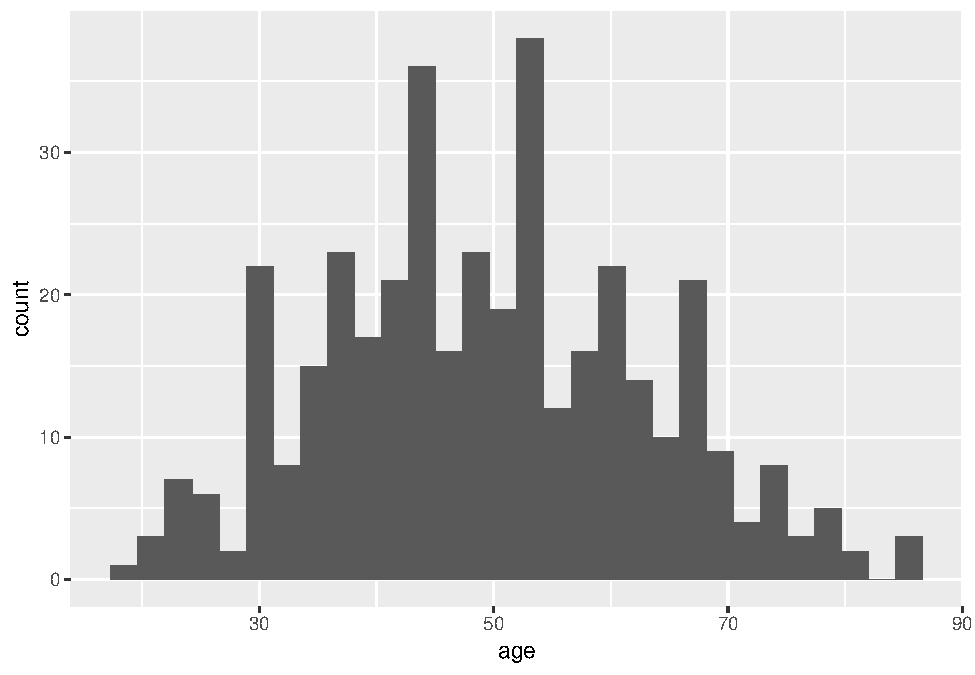
\includegraphics{02-week2_files/figure-latex/section2m-1.pdf}

\texttt{ggplot} indicates that you want to create a graph. The dataset \texttt{lesson1a} is specified in the \texttt{data} option, and \texttt{aes(x\ =\ age)} means that the variable on the x-axis should be age. \texttt{geom\_histogram} takes this data and graphs it as a histogram.

One of things that R does is to choose the number of bars for you. You can set this yourself by using the \texttt{bins} option. Try setting the number of bins to 40.

\begin{Shaded}
\begin{Highlighting}[]
\KeywordTok{ggplot}\NormalTok{(}\DataTypeTok{data =}\NormalTok{ lesson1a,}
       \KeywordTok{aes}\NormalTok{(}\DataTypeTok{x =}\NormalTok{ age)) }\OperatorTok{+}
\StringTok{  }\KeywordTok{geom_histogram}\NormalTok{(}\DataTypeTok{bins =} \DecValTok{40}\NormalTok{)}
\end{Highlighting}
\end{Shaded}

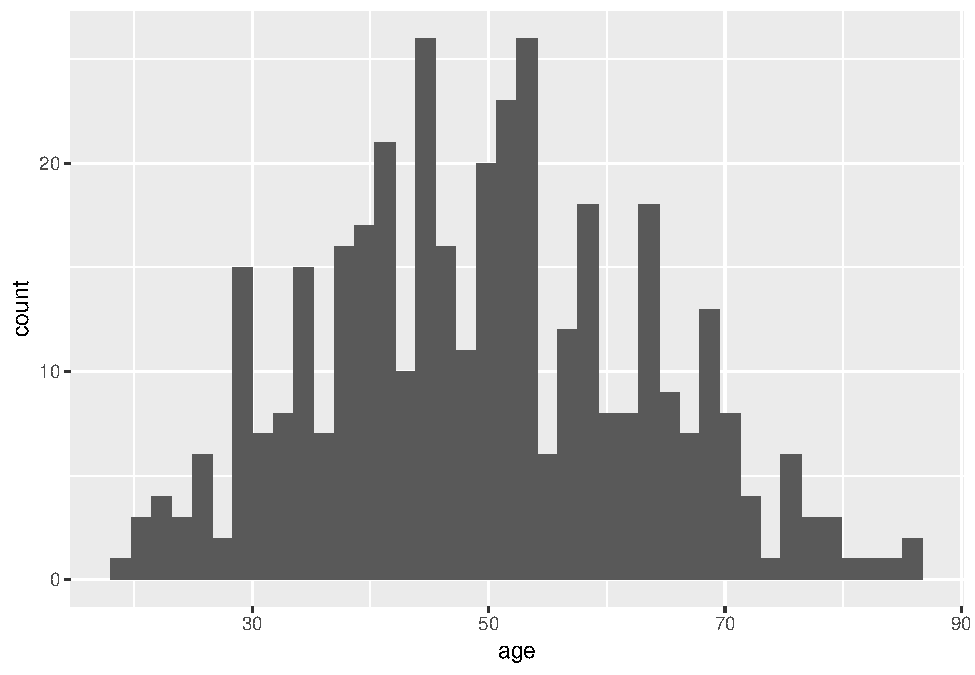
\includegraphics{02-week2_files/figure-latex/section2n-1.pdf}

The graph looks ``lumpy'' because you are breaking the data up into too many small pieces.

The following code will superimpose a curve for the normal distribution.

\begin{Shaded}
\begin{Highlighting}[]
\KeywordTok{ggplot}\NormalTok{(}\DataTypeTok{data =}\NormalTok{ lesson1a,}
       \KeywordTok{aes}\NormalTok{(}\DataTypeTok{x =}\NormalTok{ age)) }\OperatorTok{+}
\StringTok{  }\KeywordTok{geom_histogram}\NormalTok{(}\KeywordTok{aes}\NormalTok{(}\DataTypeTok{y =}\NormalTok{ ..density..), }\DataTypeTok{bins =} \DecValTok{20}\NormalTok{) }\OperatorTok{+}
\StringTok{  }\KeywordTok{geom_density}\NormalTok{()}
\end{Highlighting}
\end{Shaded}

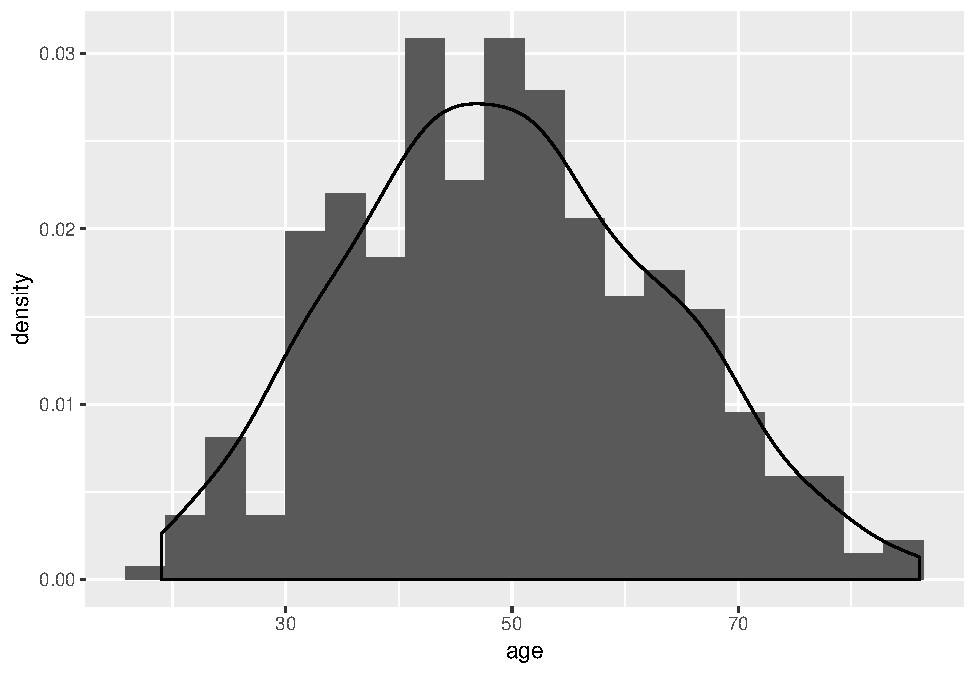
\includegraphics{02-week2_files/figure-latex/section2o-1.pdf}

\hypertarget{further-reading}{%
\subsection{Further Reading}\label{further-reading}}

Only read this if you are feeling really keen\ldots{}

\begin{Shaded}
\begin{Highlighting}[]
\CommentTok{# The "ci" function is from the "gmodels" package}

\KeywordTok{ci}\NormalTok{(lesson1a}\OperatorTok{$}\NormalTok{age, }\DataTypeTok{confidence =} \FloatTok{0.90}\NormalTok{, }\DataTypeTok{na.rm =} \OtherTok{TRUE}\NormalTok{)}
\end{Highlighting}
\end{Shaded}

\begin{verbatim}
##   Estimate   CI lower   CI upper Std. Error 
## 49.4844560 48.3301266 50.6387853  0.7000938
\end{verbatim}

This gives the mean of age, its standard error and its 90\% confidence interval (I'll explain confidence intervals next week: one thing you might want to think about is to compare the two numbers given for the confidence interval with the 5\% and 95\% centile using \texttt{quantile(lesson1a\$age)}).

\begin{Shaded}
\begin{Highlighting}[]
\KeywordTok{ci.binom}\NormalTok{(lesson1a}\OperatorTok{$}\NormalTok{sex, }\DataTypeTok{na.rm =} \OtherTok{TRUE}\NormalTok{)}
\end{Highlighting}
\end{Shaded}

\begin{verbatim}
##       Estimate  CI lower  CI upper Std. Error
## [1,] 0.5310881 0.4799345 0.5817614 0.02540009
\end{verbatim}

For a binary variable, the function \texttt{ci.binom} from the \texttt{gmodels} package is used. This gives the proportion of women along with 95\% confidence intervals (95\% is the default, meaning if you don't specify a level, it assumes you want the 95\% confidence interval.)

\hypertarget{using-r-as-a-calculator}{%
\subsection{Using R as a calculator}\label{using-r-as-a-calculator}}

R can be used as a calculator:

\begin{Shaded}
\begin{Highlighting}[]
\DecValTok{7}\OperatorTok{*}\DecValTok{7}
\end{Highlighting}
\end{Shaded}

\begin{verbatim}
## [1] 49
\end{verbatim}

\texttt{log()} is the natural logarithm (to base e)

\begin{Shaded}
\begin{Highlighting}[]
\KeywordTok{log}\NormalTok{(}\FloatTok{2.71828}\NormalTok{)}
\end{Highlighting}
\end{Shaded}

\begin{verbatim}
## [1] 0.9999993
\end{verbatim}

\texttt{exp()} is the inverse natural logarithm, that is, if exp(x)=y, e\textsuperscript{y}=x

\begin{Shaded}
\begin{Highlighting}[]
\KeywordTok{exp}\NormalTok{(}\DecValTok{1}\NormalTok{)}
\end{Highlighting}
\end{Shaded}

\begin{verbatim}
## [1] 2.718282
\end{verbatim}

\texttt{log10()} gives the log to base 10

\begin{Shaded}
\begin{Highlighting}[]
\KeywordTok{log10}\NormalTok{(}\DecValTok{100}\NormalTok{)}
\end{Highlighting}
\end{Shaded}

\begin{verbatim}
## [1] 2
\end{verbatim}

\texttt{cos(45)} gives the cosine of 45

\begin{Shaded}
\begin{Highlighting}[]
\KeywordTok{cos}\NormalTok{(}\DecValTok{45}\NormalTok{)}
\end{Highlighting}
\end{Shaded}

\begin{verbatim}
## [1] 0.525322
\end{verbatim}

Some of the functions give useful statistical constants.

\texttt{pnorm(x)} gives the probability that an observation will be less than mean + \texttt{x} standard deviations.

\begin{Shaded}
\begin{Highlighting}[]
\KeywordTok{pnorm}\NormalTok{(}\DecValTok{1}\NormalTok{)}
\end{Highlighting}
\end{Shaded}

\begin{verbatim}
## [1] 0.8413447
\end{verbatim}

\begin{Shaded}
\begin{Highlighting}[]
\KeywordTok{pnorm}\NormalTok{(}\OperatorTok{-}\FloatTok{0.5}\NormalTok{)}
\end{Highlighting}
\end{Shaded}

\begin{verbatim}
## [1] 0.3085375
\end{verbatim}

\texttt{pnorm(1)} gives 0.84 - this means that 84\% of a normally distributed set of data will be less than one standard deviation above the mean.

\texttt{pnorm(-0.5)} gives 0.31, meaning that 31\% of a normally distributed set of data will be less than half a standard deviation below the mean.

If you had a pain score with a mean of 5 and a standard deviation of 2, you could predict that only 16\% of patients would have pain scores of 7 or more and that 70\% would have pain scores of 4 or more.

\begin{Shaded}
\begin{Highlighting}[]
\KeywordTok{pnorm}\NormalTok{(}\FloatTok{1.96}\NormalTok{)}
\end{Highlighting}
\end{Shaded}

\begin{verbatim}
## [1] 0.9750021
\end{verbatim}

\begin{Shaded}
\begin{Highlighting}[]
\KeywordTok{pnorm}\NormalTok{(}\OperatorTok{-}\FloatTok{1.96}\NormalTok{)}
\end{Highlighting}
\end{Shaded}

\begin{verbatim}
## [1] 0.0249979
\end{verbatim}

\texttt{pnorm(1.96)} gives 0.975 and \texttt{pnorm(-1.96)} gives 0.025. So 97.5\% of observations are less than 1.96 standard deviations greater than the mean, and 2.5\% are less than 1.96 standard deviations lower than the mean. In other words, 95\% of observations are within 1.96 standard deviations of the mean.

\hypertarget{assignment}{%
\section{Assignment}\label{assignment}}

It seems like a lot of them, but the task shouldn't take you very long. However, a general rule in this class is: you don't have to do all the questions in the assignment. Try to do at least some (say, at least 2a and 2b), so that you know what we are talking about next week in class. Also, the more you do the more you'll learn. However, don't drive yourself crazy trying to get them all done.

I am phrasing the questions in ordinary English, pretty much as you would do if you were an investigator. For example, I ask you to summarize the data on race time in marathon runners, rather than say: ``provide the mean of the variable \texttt{rt} by typing \texttt{skim(lesson2a\$rt)}''. But this means you are going to have to work out what the various variable codes are and what commands to use.

All of these questions ask you to ``summarize'' data. In other words, how would you describe the data in a journal article (say, your table 1)? One quick clue here: I don't ever want the standard error, we'll talk more about that next week.

\hypertarget{assignments-1}{%
\subsection{Assignments}\label{assignments-1}}

\begin{itemize}
\tightlist
\item
  lesson2a.rds: This is data from marathon runners: summarize age, sex, race time in minutes (i.e.~how long it took them to complete the race) and favorite running shoe
\item
  lesson2b.rds: Postoperative pain (this is a similar data set as you had before for the assignment for the first class). Summarize average pain after the operation. Imagine you had to draw a graph of ``time course of pain after surgery''. What numbers would you use for pain at time 1, time 2, time 3 etc.?
\item
  lesson2c.rds: This is data on 242 patients undergoing radical prostatectomy. Summarize age, stage, grade and PSA.
\item
  lesson2d.rds: Cost of a minor medical procedure. Summarize cost.
\item
  lesson2e.rds: Total cancer pain in one month in a group with chronic cancer pain. Summarize pain scores and number of days with pain.
\end{itemize}

\hypertarget{week-3}{%
\chapter{Week 3}\label{week-3}}

\hypertarget{r-instructions-2}{%
\section{R Instructions}\label{r-instructions-2}}

For this lesson, make sure you have loaded the following packages.

\begin{Shaded}
\begin{Highlighting}[]
\KeywordTok{library}\NormalTok{(skimr)}
\KeywordTok{library}\NormalTok{(gtsummary)}
\KeywordTok{library}\NormalTok{(epiR)}
\KeywordTok{library}\NormalTok{(broom)}
\KeywordTok{library}\NormalTok{(pROC)}
\KeywordTok{library}\NormalTok{(gmodels)}
\KeywordTok{library}\NormalTok{(survival)}
\KeywordTok{library}\NormalTok{(tidyverse)}
\end{Highlighting}
\end{Shaded}

For this week's assignment, you will need to learn the following functions:

\begin{itemize}
\tightlist
\item
  \texttt{t.test}
\item
  \texttt{wilcox.test}
\item
  \texttt{binom.test}
\end{itemize}

\textbf{1. t-test}

This is used to compare a continuous outcome (such as hemoglobin) in two groups (e.g.~vegetarians and carnivores, or patients in a randomized trial receiving an anemia treatment or placebo). Now statistician normally say that the t-test makes two assumptions: (1) data are normally distributed and (2) variances are equal. Don't worry about assumption (2) for now. Also, assumption (1) has an odd feature: it doesn't matter once sample sizes get large (for those of you who want to boast that you know a ``theorem'', this is called the ``central limit theorem''). Just how large is ``large'' is a matter of judgment, but generally speaking, it is said that you can feel okay using a t-test on non-normal data once the sample size is above 30 a group. As it turns out, the t-test is ``robust'' to non-normal data, even if sample sizes are low. ``Robust'' means that it gives similar results regardless of whether the data are normally distributed or not. So many people feel comfortable using the t-test for just about any situation.

\textbf{Different forms of the t-test}

In a simple unpaired case, for example, testing marker levels between a drug and placebo group:

\begin{Shaded}
\begin{Highlighting}[]
\KeywordTok{t.test}\NormalTok{(marker }\OperatorTok{~}\StringTok{ }\NormalTok{trt, }\DataTypeTok{data =}\NormalTok{ trial, }\DataTypeTok{var.equal =} \OtherTok{TRUE}\NormalTok{)}
\end{Highlighting}
\end{Shaded}

\begin{verbatim}
## 
##  Two Sample t-test
## 
## data:  marker by trt
## t = -0.51222, df = 189, p-value = 0.6091
## alternative hypothesis: true difference in means is not equal to 0
## 95 percent confidence interval:
##  -0.3092384  0.1817462
## sample estimates:
##    mean in group Drug mean in group Placebo 
##             0.8981078             0.9618539
\end{verbatim}

A paired test, for example, comparing blood pressure taken before and after an intervention.

\begin{Shaded}
\begin{Highlighting}[]
\KeywordTok{t.test}\NormalTok{(bp }\OperatorTok{~}\StringTok{ }\NormalTok{when, }\DataTypeTok{data =}\NormalTok{ example3a, }\DataTypeTok{var.equal =} \OtherTok{TRUE}\NormalTok{, }\DataTypeTok{paired =} \OtherTok{TRUE}\NormalTok{)}
\end{Highlighting}
\end{Shaded}

\begin{verbatim}
## 
##  Paired t-test
## 
## data:  bp by when
## t = -3.3372, df = 119, p-value = 0.00113
## alternative hypothesis: true difference in means is not equal to 0
## 95 percent confidence interval:
##  -8.112776 -2.070557
## sample estimates:
## mean of the differences 
##               -5.091667
\end{verbatim}

A single sample test comparing the mean of a group of observations with some hypothetical value, for example, is the average rate of college-educated adults in the midwest different than the national average of 32\%?

\begin{Shaded}
\begin{Highlighting}[]
\KeywordTok{t.test}\NormalTok{(midwest}\OperatorTok{$}\NormalTok{percollege, }\DataTypeTok{mu =} \DecValTok{32}\NormalTok{)}
\end{Highlighting}
\end{Shaded}

\begin{verbatim}
## 
##  One Sample t-test
## 
## data:  midwest$percollege
## t = -45.827, df = 436, p-value < 2.2e-16
## alternative hypothesis: true mean is not equal to 32
## 95 percent confidence interval:
##  17.68400 18.86147
## sample estimates:
## mean of x 
##  18.27274
\end{verbatim}

Let's look at the print out from a t-test in more detail:

\begin{Shaded}
\begin{Highlighting}[]
\KeywordTok{t.test}\NormalTok{(hp }\OperatorTok{~}\StringTok{ }\NormalTok{am, }\DataTypeTok{data =}\NormalTok{ mtcars, }\DataTypeTok{var.equal =} \OtherTok{TRUE}\NormalTok{)}
\end{Highlighting}
\end{Shaded}

\begin{verbatim}
## 
##  Two Sample t-test
## 
## data:  hp by am
## t = 1.3733, df = 30, p-value = 0.1798
## alternative hypothesis: true difference in means is not equal to 0
## 95 percent confidence interval:
##  -16.27768  83.11169
## sample estimates:
## mean in group 0 mean in group 1 
##        160.2632        126.8462
\end{verbatim}

This example is testing whether there is a difference in horsepower (hp) between cars with an automatic transmission (am == 0) vs manual transmission (am == 1).

The \texttt{t.test} function reports the data and variables you are testing, following by the t statistic (t), degrees of freedom (df) and p-value. Below that, it states the alternative hypothesis you are testing, prints the mean in each group, and gives the 95\% confidence interval around the difference in group means.

While for an unpaired test, the \texttt{t.test} command prints the group means in each group, you may want to report the difference between means. (For a paired test, the difference in means is reported.) The group means are stored in the \texttt{estimate} attribute of the \texttt{t.test} results.

\begin{Shaded}
\begin{Highlighting}[]
\NormalTok{hp_test <-}\StringTok{ }\KeywordTok{t.test}\NormalTok{(hp }\OperatorTok{~}\StringTok{ }\NormalTok{am, }\DataTypeTok{data =}\NormalTok{ mtcars, }\DataTypeTok{var.equal =} \OtherTok{TRUE}\NormalTok{)}
\NormalTok{hp_test}\OperatorTok{$}\NormalTok{estimate}
\end{Highlighting}
\end{Shaded}

\begin{verbatim}
## mean in group 0 mean in group 1 
##        160.2632        126.8462
\end{verbatim}

To calculate the difference in means between group 0 and group 1, you can use the \texttt{estimate} data to calculate this. The square brackets indicate which number (first mean or second mean) to take. This works to calculate the difference between group 0 and group 1, as well as between group 1 and group 0.

\begin{Shaded}
\begin{Highlighting}[]
\NormalTok{hp_test}\OperatorTok{$}\NormalTok{estimate[[}\DecValTok{1}\NormalTok{]] }\OperatorTok{-}\StringTok{ }\NormalTok{hp_test}\OperatorTok{$}\NormalTok{estimate[[}\DecValTok{2}\NormalTok{]]}
\end{Highlighting}
\end{Shaded}

\begin{verbatim}
## [1] 33.417
\end{verbatim}

\begin{Shaded}
\begin{Highlighting}[]
\NormalTok{hp_test}\OperatorTok{$}\NormalTok{estimate[[}\DecValTok{2}\NormalTok{]] }\OperatorTok{-}\StringTok{ }\NormalTok{hp_test}\OperatorTok{$}\NormalTok{estimate[[}\DecValTok{1}\NormalTok{]]}
\end{Highlighting}
\end{Shaded}

\begin{verbatim}
## [1] -33.417
\end{verbatim}

You don't need to worry about the t statistic or degrees of freedom (df). The numbers you are most interested in are the p-value, the group means, and the 95\% confidence interval.

Now we haven't discussed the 95\% confidence interval yet, but think of it in simple terms as a plausible range of true values of the difference between means. In this data, the average horsepower is 33.4 higher in cars with an automatic transmission, but it could be that, in fact, the true horsepower is between 16.3 lower or 83.1 higher in the automatic group vs the manual group.

\textbf{2. Non-parametric methods}

These are used to compare continuous outcomes in two groups. There are no assumptions about normality or variance.

Unpaired case, for example, do marker levels differ between the drug and placebo groups?

\begin{Shaded}
\begin{Highlighting}[]
\KeywordTok{wilcox.test}\NormalTok{(marker }\OperatorTok{~}\StringTok{ }\NormalTok{trt, }\DataTypeTok{data =}\NormalTok{ trial, }\DataTypeTok{correct =} \OtherTok{FALSE}\NormalTok{, }\DataTypeTok{paired =} \OtherTok{FALSE}\NormalTok{)}
\end{Highlighting}
\end{Shaded}

\begin{verbatim}
## 
##  Wilcoxon rank sum test
## 
## data:  marker by trt
## W = 4242.5, p-value = 0.4366
## alternative hypothesis: true location shift is not equal to 0
\end{verbatim}

Paired case, for example, does an intervention cause a change in a patient's blood pressure?

\begin{Shaded}
\begin{Highlighting}[]
\KeywordTok{wilcox.test}\NormalTok{(bp }\OperatorTok{~}\StringTok{ }\NormalTok{when, }\DataTypeTok{data =}\NormalTok{ example3a, }\DataTypeTok{correct =} \OtherTok{FALSE}\NormalTok{, }\DataTypeTok{exact =} \OtherTok{FALSE}\NormalTok{, }\DataTypeTok{paired =} \OtherTok{FALSE}\NormalTok{)}
\end{Highlighting}
\end{Shaded}

\begin{verbatim}
## 
##  Wilcoxon rank sum test
## 
## data:  bp by when
## W = 5551, p-value = 0.002159
## alternative hypothesis: true location shift is not equal to 0
\end{verbatim}

Single sample, for example, is the rate of college education in the midwest different than the national average (32\%)?

\begin{Shaded}
\begin{Highlighting}[]
\KeywordTok{wilcox.test}\NormalTok{(midwest}\OperatorTok{$}\NormalTok{percollege, }\DataTypeTok{mu =} \DecValTok{32}\NormalTok{, }\DataTypeTok{correct =} \OtherTok{FALSE}\NormalTok{)}
\end{Highlighting}
\end{Shaded}

\begin{verbatim}
## 
##  Wilcoxon signed rank test
## 
## data:  midwest$percollege
## V = 924, p-value < 2.2e-16
## alternative hypothesis: true location is not equal to 32
\end{verbatim}

Note here that you don't get any parameters for the groups such as means, medians or standard deviations. You also don't get an estimate for the difference between groups.

\textbf{3. The binomial test}

The binomial test compares a proportion to a hypothesized value. For example, what is the probability that an unbiased coin thrown 100 times would give a result as or more extreme than 60 heads? (This probability is equivalent to the p value).

The first argument of \texttt{binom.test} is the number of successes, then the number of total tests (total observations). The hypothesized probability is specified by the \texttt{p\ =} option - the default is 0.5 (50\%).

\begin{Shaded}
\begin{Highlighting}[]
\KeywordTok{binom.test}\NormalTok{(}\DecValTok{60}\NormalTok{, }\DecValTok{100}\NormalTok{, }\DataTypeTok{p =} \FloatTok{0.5}\NormalTok{)}
\end{Highlighting}
\end{Shaded}

\begin{verbatim}
## 
##  Exact binomial test
## 
## data:  60 and 100
## number of successes = 60, number of trials = 100, p-value =
## 0.05689
## alternative hypothesis: true probability of success is not equal to 0.5
## 95 percent confidence interval:
##  0.4972092 0.6967052
## sample estimates:
## probability of success 
##                    0.6
\end{verbatim}

The following tests whether the proportion of women (sex = 1) in the dataset is different than 50\%. \texttt{sum(lesson2a\$sex)} counts the number of observations where sex is 1. \texttt{nrow(lesson2a)} gives the total number of observations in the \texttt{lesson2a} dataset.

\begin{Shaded}
\begin{Highlighting}[]
\KeywordTok{binom.test}\NormalTok{(}\KeywordTok{sum}\NormalTok{(lesson1a}\OperatorTok{$}\NormalTok{sex), }\KeywordTok{nrow}\NormalTok{(lesson1a), }\DataTypeTok{p =} \FloatTok{0.5}\NormalTok{)}
\end{Highlighting}
\end{Shaded}

\begin{verbatim}
## 
##  Exact binomial test
## 
## data:  sum(lesson1a$sex) and nrow(lesson1a)
## number of successes = 205, number of trials = 386, p-value =
## 0.2417
## alternative hypothesis: true probability of success is not equal to 0.5
## 95 percent confidence interval:
##  0.4799345 0.5817614
## sample estimates:
## probability of success 
##              0.5310881
\end{verbatim}

This tells you that you had 386 observations, and there were 205 where sex was coded as 1, an observation proportion of 0.53. Now the ``assumed'' proportion was 0.5, giving an expected number of 193 women. These two values are quite close and the p value is 0.2.

\hypertarget{assignments-2}{%
\section{Assignments}\label{assignments-2}}

Again, more questions than you need to do, unless you're keen (also, most won't take long). Try to do at least the first three.

\begin{itemize}
\tightlist
\item
  lesson3a.rds: These are data from over 1000 patients undergoing chemotherapy reporting a nausea and vomiting score from 0 to 10 on the day of treatment. Does previous chemotherapy increase nausea scores? What about sex?
\item
  lesson3b.rds: Patients with wrist osteoarthritis are randomized to a new drug or placebo. Pain is measured before and two hours after taking a dose of the drug. Is the drug effective?
\item
  lesson3c.rds: Some postoperative pain data again. Is pain on day 2 different than pain on day 1? Is pain on day 3 different from pain on day 2?
\item
  lesson3d.rds: This is a single-arm, uncontrolled study of acupuncture for patients with neck pain. Does acupuncture increase range of motion? Just as many men as women get neck pain. Can we say anything about the sample chosen for this trial with respect to gender? The mean age of patients with neck pain is 58.2 years. Is the trial population representative with respect to age?
\item
  lesson3e.rds: These data are length of stay from two different hospitals. One of the hospitals uses a new chemotherapy regime that is said to reduce adverse events and therefore length of stay. Does the new regime decrease length of stay?
\item
  lesson3f.rds: These data are from a randomized trial on the effects of physiotherapy treatment on physical function in pediatric patients recovering from cancer surgery. Function is measured on a 100 point scale. Does physiotherapy help improve physical functioning?
\end{itemize}

\hypertarget{week-4}{%
\chapter{Week 4}\label{week-4}}

\hypertarget{r-instructions-3}{%
\section{R Instructions}\label{r-instructions-3}}

For this lesson, make sure you have loaded the following packages.

\begin{Shaded}
\begin{Highlighting}[]
\KeywordTok{library}\NormalTok{(skimr)}
\KeywordTok{library}\NormalTok{(gtsummary)}
\KeywordTok{library}\NormalTok{(epiR)}
\KeywordTok{library}\NormalTok{(broom)}
\KeywordTok{library}\NormalTok{(pROC)}
\KeywordTok{library}\NormalTok{(gmodels)}
\KeywordTok{library}\NormalTok{(survival)}
\KeywordTok{library}\NormalTok{(tidyverse)}
\end{Highlighting}
\end{Shaded}

Here are some of the commands you might use when analyzing epidemiological data or data that has a similar form. For example, if you had two variables ``diet'' (where 1 = high fat, 0 = low fat) and ``hypertension'', you could use the same forms of analysis regardless of whether you were investigating a randomized trial (dietary advice assigned randomly to patients) or an epidemiological study (patients interviewed about eating habits). You can also use these methods for lab data (e.g.~proportion of mice with a knockout versus wild type who develop a tumor).

\textbf{Tables}

The first command is the \texttt{tbl\_summary} function from the \texttt{gtsummary} package which makes a table. This was introduced in the week 1 lesson. We are interested in ``two-way'' tables. In other words, we are not interested in just how many people had hypertension, but in the number of people who had hypertension in each different category of diet. I'll use the data set for assignment 3a (\texttt{lesson3a.rds}) to illustrate these points.

\begin{Shaded}
\begin{Highlighting}[]
\KeywordTok{tbl_summary}\NormalTok{(}
\NormalTok{  lesson3a }\OperatorTok\StringTok{ }\KeywordTok{select}\NormalTok{(pc, sex),}
  \DataTypeTok{by =} \StringTok{"sex"}\NormalTok{,}
  \DataTypeTok{type =} \KeywordTok{list}\NormalTok{(}\DataTypeTok{pc =} \StringTok{"categorical"}\NormalTok{)}
\NormalTok{)}
\end{Highlighting}
\end{Shaded}

\captionsetup[table]{labelformat=empty,skip=1pt}
\begin{longtable}{lcc}
\toprule
\textbf{Characteristic}\textsuperscript{1} & \textbf{0}, N = 523 & \textbf{1}, N = 575 \\ 
\midrule
previous chemo:1 if yes &  &  \\ 
0 & 160 (51\%) & 161 (50\%) \\ 
1 & 156 (49\%) & 162 (50\%) \\ 
Unknown & 207 & 252 \\ 
\bottomrule
\end{longtable}
\vspace{-5mm}
\begin{minipage}{\linewidth}
\textsuperscript{1}Statistics presented: n (\%) \\ 
\end{minipage}

So, for example, we can see that there were 575 women, 162 had prior chemo and 161 had no prior chemo. You can see that 252 women were missing data on prior chemotherapy use. By default, the table shows the percent among all observations with non-missing data.

This table also tells us that of men, 51\% had no prior chemo, and 49\% had prior chemo.

As mentioned in lesson 2, the \texttt{tbl\_summary} command gives column percentages by default, but can also give row percents using the \texttt{row\_percent\ =\ TRUE} option:

\begin{Shaded}
\begin{Highlighting}[]
\KeywordTok{tbl_summary}\NormalTok{(}
\NormalTok{  lesson3a }\OperatorTok\StringTok{ }\KeywordTok{select}\NormalTok{(pc, sex),}
  \DataTypeTok{by =} \StringTok{"sex"}\NormalTok{,}
  \DataTypeTok{type =} \KeywordTok{list}\NormalTok{(}\DataTypeTok{pc =} \StringTok{"categorical"}\NormalTok{),}
  \DataTypeTok{row_percent =} \OtherTok{TRUE}
\NormalTok{) }\OperatorTok
\StringTok{  }\KeywordTok{add_overall}\NormalTok{(}\DataTypeTok{last =} \OtherTok{TRUE}\NormalTok{)}
\end{Highlighting}
\end{Shaded}

\captionsetup[table]{labelformat=empty,skip=1pt}
\begin{longtable}{lccc}
\toprule
\textbf{Characteristic}\textsuperscript{1} & \textbf{0}, N = 523 & \textbf{1}, N = 575 & \textbf{Overall}, N = 1098 \\ 
\midrule
previous chemo:1 if yes &  &  &  \\ 
0 & 160 (50\%) & 161 (50\%) & 321 (100\%) \\ 
1 & 156 (49\%) & 162 (51\%) & 318 (100\%) \\ 
Unknown & 207 & 252 & 459 \\ 
\bottomrule
\end{longtable}
\vspace{-5mm}
\begin{minipage}{\linewidth}
\textsuperscript{1}Statistics presented: n (\%) \\ 
\end{minipage}

So of the 318 patients who had previous chemo, 51\% were women and 49\% were men.

Now let's use the marathon data (\texttt{lesson2a.rds}) to do something more interesting. First, I created a new category called ``subfourhour'' for those runners who completed the marathon in less than four hours.

\begin{Shaded}
\begin{Highlighting}[]
\NormalTok{lesson2a <-}
\StringTok{  }\NormalTok{lesson2a }\OperatorTok
\StringTok{  }\KeywordTok{mutate}\NormalTok{(}\DataTypeTok{subfourhour =}
           \KeywordTok{if_else}\NormalTok{(rt }\OperatorTok{<=}\StringTok{ }\DecValTok{240}\NormalTok{, }\DecValTok{1}\NormalTok{, }\DecValTok{0}\NormalTok{))}
\end{Highlighting}
\end{Shaded}

The \texttt{table} function is a way to make very simple tables, which is useful for doing statistical tests, although these tables do not provide as much information (variable names, totals, percentages, etc.) as \texttt{tbl\_summary}.

\begin{Shaded}
\begin{Highlighting}[]
\KeywordTok{table}\NormalTok{(lesson2a}\OperatorTok{$}\NormalTok{subfourhour, lesson2a}\OperatorTok{$}\NormalTok{sex)}
\end{Highlighting}
\end{Shaded}

\begin{verbatim}
##    
##      0  1
##   0 30 21
##   1 36 11
\end{verbatim}

\begin{Shaded}
\begin{Highlighting}[]
\CommentTok{# The first variable is the row variable}
\CommentTok{# The second variable is the column variable}
\end{Highlighting}
\end{Shaded}

We can compare sub-four hour marathons by sex using a chi-squared test (\texttt{chisq.test} function):

\begin{Shaded}
\begin{Highlighting}[]
\KeywordTok{table}\NormalTok{(lesson2a}\OperatorTok{$}\NormalTok{subfourhour, lesson2a}\OperatorTok{$}\NormalTok{sex) }\OperatorTok
\StringTok{  }\KeywordTok{chisq.test}\NormalTok{(}\DataTypeTok{correct =} \OtherTok{FALSE}\NormalTok{)}
\end{Highlighting}
\end{Shaded}

\begin{verbatim}
## 
##  Pearson's Chi-squared test
## 
## data:  .
## X-squared = 3.513, df = 1, p-value = 0.06089
\end{verbatim}

As a note, we can also use \texttt{tbl\_summary} and the \texttt{add\_p} function (also from \texttt{gtsummary}) to get the chi-squared pvalue. In the \texttt{add\_p} function, we specify that for the variable ``subfourhour'' we want to use a chi-squared test (``chisq.test'').

TODO: PENDING BEING ABLE TO DO THIS WITHOUT CONTINUITY CORRECTION

\begin{Shaded}
\begin{Highlighting}[]
\KeywordTok{tbl_summary}\NormalTok{(}
\NormalTok{  lesson2a }\OperatorTok\StringTok{ }\KeywordTok{select}\NormalTok{(subfourhour, sex),}
  \DataTypeTok{by =} \StringTok{"sex"}\NormalTok{,}
  \DataTypeTok{type =} \KeywordTok{list}\NormalTok{(}\DataTypeTok{subfourhour =} \StringTok{"categorical"}\NormalTok{)}
\NormalTok{) }\OperatorTok
\StringTok{  }\KeywordTok{add_p}\NormalTok{(}\DataTypeTok{test =} \KeywordTok{list}\NormalTok{(}\DataTypeTok{subfourhour =} \StringTok{"chisq.test"}\NormalTok{))}
\end{Highlighting}
\end{Shaded}

\captionsetup[table]{labelformat=empty,skip=1pt}
\begin{longtable}{lccc}
\toprule
\textbf{Characteristic}\textsuperscript{1} & \textbf{0}, N = 66 & \textbf{1}, N = 32 & \textbf{p-value}\textsuperscript{2} \\ 
\midrule
subfourhour &  &  & 0.10 \\ 
0 & 30 (45\%) & 21 (66\%) &  \\ 
1 & 36 (55\%) & 11 (34\%) &  \\ 
\bottomrule
\end{longtable}
\vspace{-5mm}
\begin{minipage}{\linewidth}
\textsuperscript{1}Statistics presented: n (\%) \\ 
\textsuperscript{2}Statistical tests performed: chi-square test of independence \\ 
\end{minipage}

So whereas 55\% of men completed the race in less than four hours, only 34\% of women did so. The p value here is 0.061.

\textbf{Should you categorize a continuous variable?}

If you are interested only:

Remember that the p value when we did a ttest (\texttt{t.test(rt\ \textasciitilde{}\ sex,\ data\ =\ lesson2a,\ var.equal\ =\ TRUE)}) was 0.032. That is, the p value was lower when we kept race time as a continuous variable, than when we categorized it. The reason is that we are losing information: we are treating someone who ran the race in 2.5 hours the same as someone who ran it in 3.9 hours. So in general, you should avoid turning continuous variables into categorical variables for the purposes of statistical analysis.

\textbf{Getting estimates: risk difference, risk ratio, odds ratio}

This table gives you a pvalue, but not an estimate. For this, we need the \texttt{epi.2by2} function from the \texttt{epiR} package. This function works for ``cohort studies'' and applies equally well to formal epidemiologic studies, retrospective analysis of datasets (such as in this marathon running example) or for randomized trials. You will give the \texttt{epi.2by2} function the endpoint and the cohort (see below for more details). ``Endpoint'' will be something like cancer, response, progression, or running a marathon in under four hours. ``Cohort'' is what you think might make a difference, like a toxin, chemotherapy, a genetic mutation, or gender.

The language we've been using is a little unusual for this example. A ``case'' is running a marathon in under four hours (i.e., subfourhour == 1). ``Exposed'' means that you are a woman (i.e.~sex == 1). ``Risk'' means the proportion of patients who were a ``case''.

\textbf{Coding \texttt{epi.2by2} function}

The \texttt{epi.2by2} function takes a two-way table with the endpoint and the cohort. We can create a very simple table using the \texttt{table} function with the ``cohort'' variable first (as rows), and the ``case'' variable second (as columns).

\begin{Shaded}
\begin{Highlighting}[]
\KeywordTok{table}\NormalTok{(lesson2a}\OperatorTok{$}\NormalTok{sex, lesson2a}\OperatorTok{$}\NormalTok{subfourhour)}
\end{Highlighting}
\end{Shaded}

\begin{verbatim}
##    
##      0  1
##   0 30 36
##   1 21 11
\end{verbatim}

However, \texttt{epi.2by2} requires that the first row be the ``exposed'' group (in this case, sex == 1) and the first column be the ``case'' group (subfourhour == 1). By default, R will sort the table numerically, so by default the first table row will be the ``non-exposed'' group (sex == 0) and the first column will be the ``control'' group (subfourhour == 0).

Since the rows and columns are out of order, we should first convert the table to the correct format.

\begin{Shaded}
\begin{Highlighting}[]
\KeywordTok{matrix}\NormalTok{(}\KeywordTok{rev}\NormalTok{(}\KeywordTok{table}\NormalTok{(lesson2a}\OperatorTok{$}\NormalTok{sex, lesson2a}\OperatorTok{$}\NormalTok{subfourhour)), }\DataTypeTok{nrow =} \DecValTok{2}\NormalTok{)}
\end{Highlighting}
\end{Shaded}

\begin{verbatim}
##      [,1] [,2]
## [1,]   11   21
## [2,]   36   30
\end{verbatim}

\begin{Shaded}
\begin{Highlighting}[]
\CommentTok{# For those who are curious, here is a description of the functions above:}
\CommentTok{# "table" - creates the two-way table above}
\CommentTok{# "rev" - reverses the order of the table}
\CommentTok{# "matrix(..., nrow = 2)" converts the reversed data back into a two-by-two table}
\end{Highlighting}
\end{Shaded}

You will see here that now both the rows and the columns are reversed in this table. You can put this code directly into the \texttt{epi.2by2} function.

\begin{Shaded}
\begin{Highlighting}[]
\KeywordTok{epi.2by2}\NormalTok{(}\KeywordTok{matrix}\NormalTok{(}\KeywordTok{rev}\NormalTok{(}\KeywordTok{table}\NormalTok{(lesson2a}\OperatorTok{$}\NormalTok{sex, lesson2a}\OperatorTok{$}\NormalTok{subfourhour)), }\DataTypeTok{nrow =} \DecValTok{2}\NormalTok{))}
\end{Highlighting}
\end{Shaded}

\begin{verbatim}
##              Outcome +    Outcome -      Total        Inc risk *
## Exposed +           11           21         32              34.4
## Exposed -           36           30         66              54.5
## Total               47           51         98              48.0
##                  Odds
## Exposed +       0.524
## Exposed -       1.200
## Total           0.922
## 
## Point estimates and 95% CIs:
## -------------------------------------------------------------------
## Inc risk ratio                               0.63 (0.37, 1.07)
## Odds ratio                                   0.44 (0.18, 1.05)
## Attrib risk *                                -20.17 (-40.54, 0.20)
## Attrib risk in population *                  -6.59 (-22.15, 8.97)
## Attrib fraction in exposed (%)               -58.68 (-168.76, 6.32)
## Attrib fraction in population (%)            -13.73 (-29.44, 0.07)
## -------------------------------------------------------------------
##  Test that odds ratio = 1: chi2(1) = 3.513 Pr>chi2 = 0.061
##  Wald confidence limits
##  CI: confidence interval
##  * Outcomes per 100 population units
\end{verbatim}

So reading this table we get the following information:

\begin{itemize}
\tightlist
\item
  There were 32 women (``Exposed +'' row, ``Total'' column) and 66 men (``Exposed -'' row, ``Total'' column), a total of 98 patients (``Total'' row and column)
\item
  11 of the women finished the race in under four hours (``Exposed +'' row, ``Outcome +'' column), 21 did not (``Exposed +'' row, ``Outcome -'' column).
\item
  36 of the men finished the race in under four hours (``Exposed -'' row, ``Outcome +'' column), 30 did not (``Exposed -'' row, ``Outcome -'' column)
\item
  34.4\% of the women (``Exposed +'' column, ``Inc risk *'' row) and 54.5\% of the men (``Exposed -'' column, ``Inc risk *'' row) finished in under four hours.
\item
  20\% more men finished the race in under four hours ("Attrib risk *" under ``Point estimates and 95\% CIs''). The 95\% CI is 41\% more to 0.20\% less.
\item
  The chance that a woman finishes the race in under four hours is 0.63 of that for a man (``Inc risk ratio'' under ``Point estimates and 95\% CIs''). The 95\% CI is 0.37 to 1.07 (i.e about one third as likely to 7\% more likely).
\item
  The odds ratio is reported in the second row under ``Point estimates and 95\% CIs.''
\end{itemize}

Here is another one to look through:

\begin{Shaded}
\begin{Highlighting}[]
\KeywordTok{epi.2by2}\NormalTok{(}\KeywordTok{matrix}\NormalTok{(}\KeywordTok{rev}\NormalTok{(}\KeywordTok{table}\NormalTok{(example4a}\OperatorTok{$}\NormalTok{toxin, example4a}\OperatorTok{$}\NormalTok{cancer)), }\DataTypeTok{nrow =} \DecValTok{2}\NormalTok{))}
\end{Highlighting}
\end{Shaded}

\begin{verbatim}
##              Outcome +    Outcome -      Total        Inc risk *
## Exposed +            5            3          8              62.5
## Exposed -            1            7          8              12.5
## Total                6           10         16              37.5
##                  Odds
## Exposed +       1.667
## Exposed -       0.143
## Total           0.600
## 
## Point estimates and 95% CIs:
## -------------------------------------------------------------------
## Inc risk ratio                               5.00 (0.74, 33.78)
## Odds ratio                                   11.67 (0.92, 147.56)
## Attrib risk *                                50.00 (9.37, 90.63)
## Attrib risk in population *                  25.00 (-7.98, 57.98)
## Attrib fraction in exposed (%)               80.00 (-35.11, 97.04)
## Attrib fraction in population (%)            66.67 (-69.30, 93.44)
## -------------------------------------------------------------------
##  Test that odds ratio = 1: chi2(1) = 4.267 Pr>chi2 = 0.039
##  Wald confidence limits
##  CI: confidence interval
##  * Outcomes per 100 population units
\end{verbatim}

Here it is easier to see that the ``toxin'' is the exposure and ``cancer'' is whether you are a case.

\textbf{Exact statistics}

Now I'll explain what these are in more detail in the box below for whoever is interested. But for now, what everyone needs to now is that many statisticians, myself included, prefer exact statistics and if any of the ``cells'' in your table have five or fewer observations, all statisticians agree that you should use exact methods. A cell is one box in your table, such as the number of cancer patients who were not exposed to the toxin, or the number of non-cancer patients who were exposed to the toxin. The \texttt{epi.2by2} function gives the chi-squared p-value. However, using the \texttt{fisher.test} function gives the exact pvalue.

\begin{Shaded}
\begin{Highlighting}[]
\KeywordTok{fisher.test}\NormalTok{(}\KeywordTok{table}\NormalTok{(example4a}\OperatorTok{$}\NormalTok{toxin, example4a}\OperatorTok{$}\NormalTok{cancer))}
\end{Highlighting}
\end{Shaded}

\begin{verbatim}
## 
##  Fisher's Exact Test for Count Data
## 
## data:  table(example4a$toxin, example4a$cancer)
## p-value = 0.1189
## alternative hypothesis: true odds ratio is not equal to 1
## 95 percent confidence interval:
##    0.6795665 625.2181311
## sample estimates:
## odds ratio 
##   9.760631
\end{verbatim}

\begin{Shaded}
\begin{Highlighting}[]
\CommentTok{# Note - you do not need to reverse the row/column order for the "fisher.test" function}
\end{Highlighting}
\end{Shaded}

Similar to the chi-squared test, you can also get the Fisher's exact pvalue using the \texttt{tbl\_summary} and \texttt{add\_p} functions, by specifying \texttt{test\ =\ "fisher.test"} for the variable of interest.

\begin{Shaded}
\begin{Highlighting}[]
\KeywordTok{tbl_summary}\NormalTok{(}
\NormalTok{  example4a }\OperatorTok\StringTok{ }\KeywordTok{select}\NormalTok{(toxin, cancer),}
  \DataTypeTok{by =} \StringTok{"cancer"}\NormalTok{,}
  \DataTypeTok{type =} \KeywordTok{list}\NormalTok{(}\DataTypeTok{toxin =} \StringTok{"categorical"}\NormalTok{)}
\NormalTok{) }\OperatorTok
\StringTok{  }\KeywordTok{add_p}\NormalTok{(}\DataTypeTok{test =} \KeywordTok{list}\NormalTok{(}\DataTypeTok{toxin =} \StringTok{"fisher.test"}\NormalTok{))}
\end{Highlighting}
\end{Shaded}

\captionsetup[table]{labelformat=empty,skip=1pt}
\begin{longtable}{lccc}
\toprule
\textbf{Characteristic}\textsuperscript{1} & \textbf{0}, N = 10 & \textbf{1}, N = 6 & \textbf{p-value}\textsuperscript{2} \\ 
\midrule
Toxin exposure &  &  & 0.12 \\ 
0 & 7 (70\%) & 1 (17\%) &  \\ 
1 & 3 (30\%) & 5 (83\%) &  \\ 
\bottomrule
\end{longtable}
\vspace{-5mm}
\begin{minipage}{\linewidth}
\textsuperscript{1}Statistics presented: n (\%) \\ 
\textsuperscript{2}Statistical tests performed: Fisher\textquotesingle{}s exact test \\ 
\end{minipage}

\emph{For keen students only:}

Let's imagine that you and I each throw two coins. I throw two heads and you throw two tails. The p value you get from a chi squared is 0.046, which seems strange as what we threw doesn't seem that unusual. The problem is that in chi squared analysis you compare the expected and observed values, add them up, get a value for chi, and then look this up on a table. Now this table is derived from a distribution based on large samples. It is an approximation that breaks down when numbers are very small (such as less than 5 in at least one cell). ``Exact'' statistics works out the probability of a certain result in a different way, without reference to distributions or approximations.

The exact approach to the coin throwing problem would be to write out all the possible tables you could have with four observations, and then work out the probability of each under the null hypothesis. Then count what proportion of tables are as unlikely or more unlikely than the observed results and you get your p value. It turns out that there are 9 possible outcomes for the coin throwing problem: 0 vs.~0; 0 vs 1; 0 vs.~2; 1 vs.~0; 1 vs.~1; 1 vs.~2; 2 vs.~0; 2 vs 1; 2 vs.~2. Two of these (0 vs.~2 and 2 vs.~0), are at least as extreme as the result we got, so that gives a p value of 0.33.

\textbf{Other Commands}

You can use the \texttt{filter} command to select rows to perform ttests on subgroups of your data. For example, to assess the association between nausea/vomiting and sex only among those patients who had a history of prior chemotherapy, you can use the following code:

\begin{Shaded}
\begin{Highlighting}[]
\KeywordTok{t.test}\NormalTok{(nv }\OperatorTok{~}\StringTok{ }\NormalTok{sex, }\DataTypeTok{data =}\NormalTok{ lesson3a }\OperatorTok\StringTok{ }\KeywordTok{filter}\NormalTok{(pc}\OperatorTok{==}\DecValTok{1}\NormalTok{))}
\end{Highlighting}
\end{Shaded}

\begin{verbatim}
## 
##  Welch Two Sample t-test
## 
## data:  nv by sex
## t = -0.078122, df = 251.57, p-value = 0.9378
## alternative hypothesis: true difference in means is not equal to 0
## 95 percent confidence interval:
##  -0.5219692  0.4821391
## sample estimates:
## mean in group 0 mean in group 1 
##        5.270161        5.290076
\end{verbatim}

To perform the ttest on those without prior chemotherapy, switch the group you are filtering on:

\begin{Shaded}
\begin{Highlighting}[]
\KeywordTok{t.test}\NormalTok{(nv }\OperatorTok{~}\StringTok{ }\NormalTok{sex, }\DataTypeTok{data =}\NormalTok{ lesson3a }\OperatorTok\StringTok{ }\KeywordTok{filter}\NormalTok{(pc}\OperatorTok{==}\DecValTok{0}\NormalTok{))}
\end{Highlighting}
\end{Shaded}

\begin{verbatim}
## 
##  Welch Two Sample t-test
## 
## data:  nv by sex
## t = 0.2822, df = 254.8, p-value = 0.778
## alternative hypothesis: true difference in means is not equal to 0
## 95 percent confidence interval:
##  -0.4171295  0.5566757
## sample estimates:
## mean in group 0 mean in group 1 
##        4.492537        4.422764
\end{verbatim}

\hypertarget{assignments-3}{%
\section{Assignments}\label{assignments-3}}

This week's assignment concerns techniques developed to assess epidemiologic data. But remember that a number is just a number: the techniques for working out the relative risk of getting breast cancer if you has a silicone breast implant is exactly the same as working out the relative risk of death in transgenic mice exposed to a carcinogen.

Try to do the ones in bold, get to the non-bolded ones if you can.

\begin{itemize}
\tightlist
\item
  \textbf{lesson4a.rds: This is a data set on fifteen patients recording whether they had problematic nausea or vomiting after chemotherapy (defined as grade 2 or higher for either nausea or vomiting) and whether they reported being prone to travel sickness. Does travel sickness predict chemotherapy nausea and vomiting?}
\item
  lesson4b.rds: An epidemiological study of meat consumption and hypertension in older Americans. Meat consumption was defined as low, medium or high depending on whether subjects ate less than 3, 3 to 7 or 7 + meals with meat in per week. Does meat consumption lead to hypertension?
\item
  lesson4c.rds: This is a data set from a chemotherapy study. The researchers think that a mutation of a certain gene may be associated with chemotherapy toxicity. Should clinicians test for the gene during pre-chemotherapy work up?
\item
  \textbf{lesson4d.rds: Patients with lung cancer are randomized to receive either chemotherapy regimen a or b and assessed for tumor response. Which regimen would you recommend to a patient? Do the treatments work differently depending on age or sex?}
\item
  lesson4e.rds: This is a lab study of two candidate tumor-suppressor genes (gene1 and gene2). Wild-type mice are compared with mice that have gene1 knocked-out, gene2 knocked-out or both. The presence of tumors is measured after 30 days. Do the genes suppress cancer?
\end{itemize}

\hypertarget{week-5}{%
\chapter{Week 5}\label{week-5}}

\hypertarget{r-instructions-4}{%
\section{R Instructions}\label{r-instructions-4}}

For this lesson, make sure you have loaded the following packages.

\begin{Shaded}
\begin{Highlighting}[]
\KeywordTok{library}\NormalTok{(skimr)}
\KeywordTok{library}\NormalTok{(gtsummary)}
\KeywordTok{library}\NormalTok{(epiR)}
\KeywordTok{library}\NormalTok{(broom)}
\KeywordTok{library}\NormalTok{(pROC)}
\KeywordTok{library}\NormalTok{(gmodels)}
\KeywordTok{library}\NormalTok{(survival)}
\KeywordTok{library}\NormalTok{(tidyverse)}
\end{Highlighting}
\end{Shaded}

\hypertarget{correlation}{%
\subsection{Correlation}\label{correlation}}

Correlating two or more variables is very easy: just use the \texttt{cor} function and then the dataset and selected variables.

For example, if you use the \texttt{lesson2b.rds} dataset and correlate the first four pain scores, you get the following table:

\begin{Shaded}
\begin{Highlighting}[]
\KeywordTok{cor}\NormalTok{(lesson2b }\OperatorTok\StringTok{ }\KeywordTok{select}\NormalTok{(l01, l02, l03, l04))}
\end{Highlighting}
\end{Shaded}

\begin{verbatim}
##           l01       l02       l03       l04
## l01 1.0000000 0.7900984 0.6270860 0.5395075
## l02 0.7900984 1.0000000 0.8145025 0.7148299
## l03 0.6270860 0.8145025 1.0000000 0.8383224
## l04 0.5395075 0.7148299 0.8383224 1.0000000
\end{verbatim}

\begin{Shaded}
\begin{Highlighting}[]
\CommentTok{# The "select" function allows you to keep specific columns from your dataset}
\end{Highlighting}
\end{Shaded}

This shows, for example, that the correlation between l01 and l02 is 0.79 and the correlation between l02 and l04 is 0.71. From the table you can easily see that pain scores taken on consecutive days are more strongly correlated than those taken two or three days apart.

If the data are skewed, you can try a regression based on ranks, what is known as Spearman's rank correlation. What you'd type is the same as above, but adding the option \texttt{method\ =\ "spearman"}.

\begin{Shaded}
\begin{Highlighting}[]
\KeywordTok{cor}\NormalTok{(lesson2b }\OperatorTok\StringTok{ }\KeywordTok{select}\NormalTok{(l01, l02, l03, l04), }\DataTypeTok{method =} \StringTok{"spearman"}\NormalTok{)}
\end{Highlighting}
\end{Shaded}

\begin{verbatim}
##           l01       l02       l03       l04
## l01 1.0000000 0.7799856 0.6220233 0.5443327
## l02 0.7799856 1.0000000 0.8126008 0.7220277
## l03 0.6220233 0.8126008 1.0000000 0.8324906
## l04 0.5443327 0.7220277 0.8324906 1.0000000
\end{verbatim}

\hypertarget{linear-regression}{%
\subsection{Linear regression}\label{linear-regression}}

Linear regression is when you try to predict a continuous variable. The function to use is \texttt{lm}.

The first variable is the dependent variable (e.g.~blood pressure) and must be continuous. The other variables are the predictor variables and can be binary or continuous: in some cases you can use ordinal variables but you have to be careful. We'll deal with categorical variables later in the course. The dependent and predictor variables are separated by a ``\textasciitilde{}'', and multiple predictor variables are separated by ``+''.

Let's use the data from \texttt{lesson3d.rds} as an example dataset. We want to see if we can predict a patient's range of motion after treatment (variable a) in terms of their age, sex and pre-treatment range of motion (variable b).

\begin{Shaded}
\begin{Highlighting}[]
\KeywordTok{lm}\NormalTok{(a }\OperatorTok{~}\StringTok{ }\NormalTok{sex }\OperatorTok{+}\StringTok{ }\NormalTok{age }\OperatorTok{+}\StringTok{ }\NormalTok{b, }\DataTypeTok{data =}\NormalTok{ lesson3d)}
\end{Highlighting}
\end{Shaded}

\begin{verbatim}
## 
## Call:
## lm(formula = a ~ sex + age + b, data = lesson3d)
## 
## Coefficients:
## (Intercept)          sex          age            b  
##    138.7336       2.8524      -0.4359       0.6692
\end{verbatim}

This gives you the very basic information from the regression, but you can get more information using the \texttt{summary} function:

\begin{Shaded}
\begin{Highlighting}[]
\NormalTok{rom_model <-}\StringTok{ }\KeywordTok{lm}\NormalTok{(a }\OperatorTok{~}\StringTok{ }\NormalTok{sex }\OperatorTok{+}\StringTok{ }\NormalTok{age }\OperatorTok{+}\StringTok{ }\NormalTok{b, }\DataTypeTok{data =}\NormalTok{ lesson3d)}
\KeywordTok{summary}\NormalTok{(rom_model)}
\end{Highlighting}
\end{Shaded}

\begin{verbatim}
## 
## Call:
## lm(formula = a ~ sex + age + b, data = lesson3d)
## 
## Residuals:
##     Min      1Q  Median      3Q     Max 
## -60.135 -11.943   3.238  14.523  47.732 
## 
## Coefficients:
##              Estimate Std. Error t value Pr(>|t|)    
## (Intercept) 138.73363   29.50514   4.702 5.40e-05 ***
## sex           2.85241   10.25817   0.278    0.783    
## age          -0.43589    0.27770  -1.570    0.127    
## b             0.66924    0.07816   8.563 1.49e-09 ***
## ---
## Signif. codes:  0 '***' 0.001 '**' 0.01 '*' 0.05 '.' 0.1 ' ' 1
## 
## Residual standard error: 25.29 on 30 degrees of freedom
## Multiple R-squared:  0.7475, Adjusted R-squared:  0.7222 
## F-statistic:  29.6 on 3 and 30 DF,  p-value: 4.241e-09
\end{verbatim}

The first column of numbers listed under ``Coefficients'' are the coefficients. You can interpret this as follows: start with 138.7 degrees of range of motion (the intercept or constant). Then add 2.85 if the patient is a woman, and take away 0.436 degrees for every year of age. Find, add 0.669 degrees for every degree of range of motion the patient had before the trial.

Let's take a single patient: a 54 year old woman with a range of motion of 301 before treatment. Her predicted range of motion afterwards is 138.7 + 2.85 - 0.436*54 + 0.669*301 = 319.5. Her actual figure was 325, so we predicted quite well for this patient. You can get R to do this automatically using the \texttt{augment} function from the \texttt{broom} package.

\begin{Shaded}
\begin{Highlighting}[]
\CommentTok{# The "augment" function creates a dataset of all patients included in the model}
\CommentTok{# and all variables included in the model, as well as the predictions}
\CommentTok{# The ".fitted" column is your prediction}

\NormalTok{lesson3d_pred <-}
\StringTok{  }\KeywordTok{augment}\NormalTok{(rom_model,}
          \DataTypeTok{newdata =}\NormalTok{ lesson3d)}
\end{Highlighting}
\end{Shaded}

To get the number of observations, coefficients, 95\% confidence interval and p-values printed in a table for all covariates, you can use the \texttt{tbl\_regression} function from the \texttt{gtsummary} package:

\begin{Shaded}
\begin{Highlighting}[]
\KeywordTok{tbl_regression}\NormalTok{(rom_model)}
\end{Highlighting}
\end{Shaded}

\captionsetup[table]{labelformat=empty,skip=1pt}
\begin{longtable}{lccc}
\toprule
\textbf{N = 34} & \textbf{Coefficient} & \textbf{95\% CI}\textsuperscript{1} & \textbf{p-value} \\ 
\midrule
1=female & 2.9 & -18, 24 & 0.8 \\ 
age & -0.44 & -1.0, 0.13 & 0.13 \\ 
range of motion before acupuncture & 0.67 & 0.51, 0.83 & <0.001 \\ 
\bottomrule
\end{longtable}
\vspace{-5mm}
\begin{minipage}{\linewidth}
\textsuperscript{1}CI = Confidence Interval \\ 
\end{minipage}

For example, for sex, the 95\% CI is -18 to 24, meaning that women might plausibly have a range of motion anywhere from 18 degrees less than men to 24 degrees more. In short, we don't have any strong evidence that sex has an effect on range of motion at all and we can see this reflected in the p value, p=0.8. There are 34 patients included in this model.

\begin{Shaded}
\begin{Highlighting}[]
\KeywordTok{summary}\NormalTok{(rom_model)}
\end{Highlighting}
\end{Shaded}

\begin{verbatim}
## 
## Call:
## lm(formula = a ~ sex + age + b, data = lesson3d)
## 
## Residuals:
##     Min      1Q  Median      3Q     Max 
## -60.135 -11.943   3.238  14.523  47.732 
## 
## Coefficients:
##              Estimate Std. Error t value Pr(>|t|)    
## (Intercept) 138.73363   29.50514   4.702 5.40e-05 ***
## sex           2.85241   10.25817   0.278    0.783    
## age          -0.43589    0.27770  -1.570    0.127    
## b             0.66924    0.07816   8.563 1.49e-09 ***
## ---
## Signif. codes:  0 '***' 0.001 '**' 0.01 '*' 0.05 '.' 0.1 ' ' 1
## 
## Residual standard error: 25.29 on 30 degrees of freedom
## Multiple R-squared:  0.7475, Adjusted R-squared:  0.7222 
## F-statistic:  29.6 on 3 and 30 DF,  p-value: 4.241e-09
\end{verbatim}

At the bottom of the \texttt{summary} readout there are a few miscellaneous tidbits:

\begin{itemize}
\item
  The ``p-value'' next to the ``F-statistic'' on the last line tells you whether, as a whole, your model, including the constant and three variables, is a statistically significant predictor.
\item
  The ``Multiple R-squared'' value (often referred to as just ``R-squared'') tells you how good a predictor it is on a scale from 0 to 1. We'll discuss the meaning of r squared in more detail, but it is defined as the proportion of variation that you can explain using your model.
\end{itemize}

\hypertarget{graphing-the-data}{%
\subsection{Graphing the data}\label{graphing-the-data}}

Graphing the data is done using the \texttt{ggplot} function from the \texttt{ggplot2} package. In short, the main inputs for the \texttt{ggplot} function are your dataset, the x variable and the y variable. You can then create a number of different plots using this data.

To create a scatterplot, the \texttt{geom\_point} function is added to the \texttt{ggplot} function:

\begin{Shaded}
\begin{Highlighting}[]
\KeywordTok{ggplot}\NormalTok{(}\DataTypeTok{data =}\NormalTok{ lesson5a,}
       \KeywordTok{aes}\NormalTok{(}\DataTypeTok{x =}\NormalTok{ age, }\DataTypeTok{y =}\NormalTok{ rt)) }\OperatorTok{+}
\StringTok{  }\KeywordTok{geom_point}\NormalTok{()}
\end{Highlighting}
\end{Shaded}

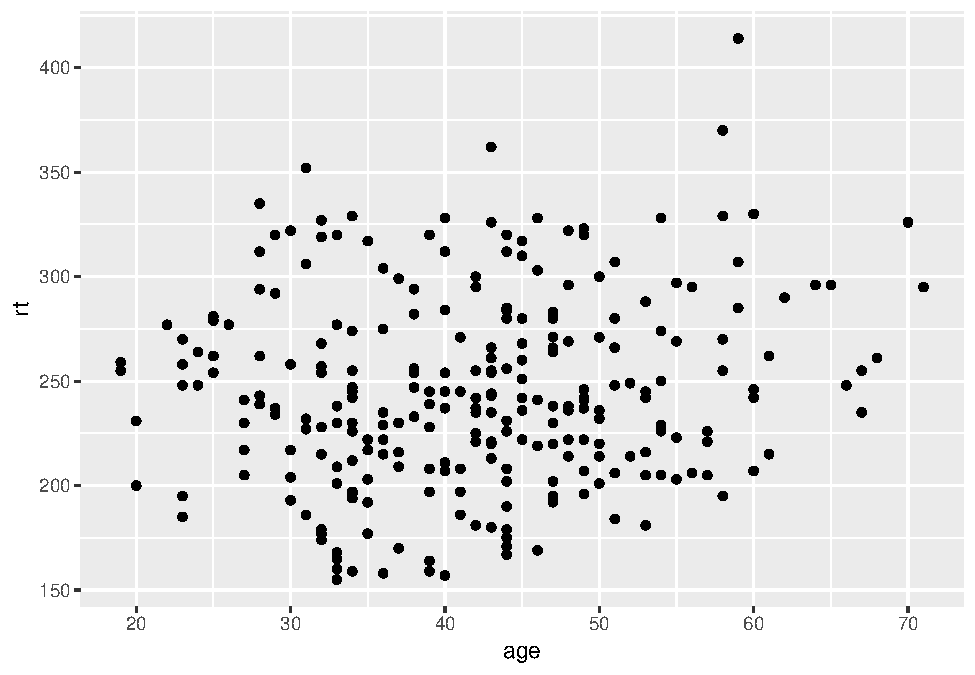
\includegraphics{05-week5_files/figure-latex/section5j-1.pdf}

This scatterplot from the \texttt{lesson5a.rds} data shows race time and age for every runner in the study. This is a useful way of getting a feel for the data before you start.

\hypertarget{logistic-regression}{%
\subsection{Logistic regression}\label{logistic-regression}}

Logistic regression is used when the variable you wish to predict is binary (e.g.~relapsed or not). The function to use is \texttt{glm}, with the option \texttt{family\ =\ "binomial"} to indicate that our outcome variable is binary.

Again, the first variable is the dependent variable (e.g.~hypertension) and must be binary. The other variables are the predictor variables and can be binary or continuous: again, in some cases you can use ordinal variables but you have to be careful. The variables are entered into the \texttt{glm} function the same way as the \texttt{lm} function (dependent \textasciitilde{} predictor1 + predictor2 + \ldots).

We'll use the dataset \texttt{lesson4d.rds} as an example.

\begin{Shaded}
\begin{Highlighting}[]
\NormalTok{response_model <-}\StringTok{ }\KeywordTok{glm}\NormalTok{(response }\OperatorTok{~}\StringTok{ }\NormalTok{age }\OperatorTok{+}\StringTok{ }\NormalTok{sex }\OperatorTok{+}\StringTok{ }\NormalTok{group, }\DataTypeTok{data =}\NormalTok{ lesson4d, }\DataTypeTok{family =} \StringTok{"binomial"}\NormalTok{)}
\KeywordTok{summary}\NormalTok{(response_model)}
\end{Highlighting}
\end{Shaded}

\begin{verbatim}
## 
## Call:
## glm(formula = response ~ age + sex + group, family = "binomial", 
##     data = lesson4d)
## 
## Deviance Residuals: 
##     Min       1Q   Median       3Q      Max  
## -1.3760  -1.0954  -0.9119   1.2366   1.5590  
## 
## Coefficients:
##              Estimate Std. Error z value Pr(>|z|)  
## (Intercept)  0.967546   0.447037   2.164   0.0304 *
## age         -0.023270   0.009807  -2.373   0.0177 *
## sex         -0.180196   0.234045  -0.770   0.4413  
## group       -0.318300   0.205037  -1.552   0.1206  
## ---
## Signif. codes:  0 '***' 0.001 '**' 0.01 '*' 0.05 '.' 0.1 ' ' 1
## 
## (Dispersion parameter for binomial family taken to be 1)
## 
##     Null deviance: 546.87  on 397  degrees of freedom
## Residual deviance: 538.18  on 394  degrees of freedom
##   (2 observations deleted due to missingness)
## AIC: 546.18
## 
## Number of Fisher Scoring iterations: 4
\end{verbatim}

By default, R gives the coefficients in logits. To easily see the coefficients and 95\% confidence intervals for all covariates as odds ratio, we can again use the \texttt{tbl\_regression} function. In this case, we use the option \texttt{exponentiate\ =\ TRUE}, which indicates that odds ratios (not logits) should be presented. (You can also use this function to see the formatted logit results by using the \texttt{exponentiate\ =\ FALSE} option.)

\begin{Shaded}
\begin{Highlighting}[]
\KeywordTok{glm}\NormalTok{(response }\OperatorTok{~}\StringTok{ }\NormalTok{age }\OperatorTok{+}\StringTok{ }\NormalTok{sex }\OperatorTok{+}\StringTok{ }\NormalTok{group, }\DataTypeTok{data =}\NormalTok{ lesson4d, }\DataTypeTok{family =} \StringTok{"binomial"}\NormalTok{) }\OperatorTok
\StringTok{  }\KeywordTok{tbl_regression}\NormalTok{(}\DataTypeTok{exponentiate =} \OtherTok{TRUE}\NormalTok{)}
\end{Highlighting}
\end{Shaded}

\captionsetup[table]{labelformat=empty,skip=1pt}
\begin{longtable}{lccc}
\toprule
\textbf{N = 398} & \textbf{OR}\textsuperscript{1} & \textbf{95\% CI}\textsuperscript{1} & \textbf{p-value} \\ 
\midrule
age & 0.98 & 0.96, 1.00 & 0.018 \\ 
1 if woman, 0 if man & 0.84 & 0.53, 1.32 & 0.4 \\ 
1 if b, 0 if a & 0.73 & 0.49, 1.09 & 0.12 \\ 
\bottomrule
\end{longtable}
\vspace{-5mm}
\begin{minipage}{\linewidth}
\textsuperscript{1}OR = Odds Ratio, CI = Confidence Interval \\ 
\end{minipage}

The key things here are the odds ratios: you can say that the odds of response is multiplied by 0.98 for a one year increase in age; that women have an odds of response 0.84 of that for the men, though this is not statistically significant, and that response is lower in group 1, with an odds of 0.73 (you would also cite the p value and 95\% CIs).

The problem here is that you can't use any of these data to work out an individual patient's chance of response. Now you can get R to do this for you using the \texttt{augment} function. For a binary outcome, you need to specify \texttt{type.predict\ =\ "response"} as an option so that you will get predicted probabilities (not log odds).

\begin{Shaded}
\begin{Highlighting}[]
\NormalTok{lesson4d_pred <-}
\StringTok{  }\KeywordTok{augment}\NormalTok{(response_model,}
          \DataTypeTok{newdata =}\NormalTok{ lesson4d,}
          \DataTypeTok{type.predict =} \StringTok{"response"}\NormalTok{)}
\end{Highlighting}
\end{Shaded}

NOTE: The \texttt{lesson4d\_pred} dataset only includes 398 patients. If you look at the table above, you will see at the top that only 398 patients were included in the model. Any patients who are missing data for the outcome or any predictors will be excluded from the model, and will not be included in the predicted dataset.

If you want to look at calculating predictions from logistic regression in more detail, you'll need logit (see below).

One thing to be careful about is categorical variables. Imagine that you had the patients age and cancer stage (1, 2, 3 or 4) and wanted to know whether they recurred. If you tried \texttt{glm(recurrence\ \textasciitilde{}\ age\ +\ stage,\ ...)}, then stage would be treated as if the increase in risk going from stage 1 to 2 was exactly the same as that going from 2 to 3 and 3 to 4. To tell R that it is a categorical variable, you need to use the \texttt{factor} function with the categorical variable:

\begin{Shaded}
\begin{Highlighting}[]
\NormalTok{recurrence_model }\OperatorTok
\StringTok{  }\KeywordTok{tbl_regression}\NormalTok{(}\DataTypeTok{exponentiate =} \OtherTok{TRUE}\NormalTok{)}
\end{Highlighting}
\end{Shaded}

\captionsetup[table]{labelformat=empty,skip=1pt}
\begin{longtable}{lccc}
\toprule
\textbf{N = 1064} & \textbf{OR}\textsuperscript{1} & \textbf{95\% CI}\textsuperscript{1} & \textbf{p-value} \\ 
\midrule
age & 1.04 & 1.03, 1.05 & <0.001 \\ 
factor(stage) &  &  &  \\ 
1 & --- & --- &  \\ 
2 & 2.71 & 2.01, 3.66 & <0.001 \\ 
3 & 5.23 & 3.16, 8.79 & <0.001 \\ 
4 & 5.88 & 3.34, 10.6 & <0.001 \\ 
\bottomrule
\end{longtable}
\vspace{-5mm}
\begin{minipage}{\linewidth}
\textsuperscript{1}OR = Odds Ratio, CI = Confidence Interval \\ 
\end{minipage}

What you can see here is that stage is broken into categories. The odds ratio is given comparing each stage to stage 1 (the reference). So the odds of recurrence is 2.71 higher for stage 2 compared to stage 1, 5.23 for stage 3 compared to stage 1 and 5.88 for stage 4 compared to stage 1.

\textbf{For keen students only!}

Here we look at our ``response'' model on the logit scale.

\begin{Shaded}
\begin{Highlighting}[]
\KeywordTok{summary}\NormalTok{(response_model)}
\end{Highlighting}
\end{Shaded}

\begin{verbatim}
## 
## Call:
## glm(formula = response ~ age + sex + group, family = "binomial", 
##     data = lesson4d)
## 
## Deviance Residuals: 
##     Min       1Q   Median       3Q      Max  
## -1.3760  -1.0954  -0.9119   1.2366   1.5590  
## 
## Coefficients:
##              Estimate Std. Error z value Pr(>|z|)  
## (Intercept)  0.967546   0.447037   2.164   0.0304 *
## age         -0.023270   0.009807  -2.373   0.0177 *
## sex         -0.180196   0.234045  -0.770   0.4413  
## group       -0.318300   0.205037  -1.552   0.1206  
## ---
## Signif. codes:  0 '***' 0.001 '**' 0.01 '*' 0.05 '.' 0.1 ' ' 1
## 
## (Dispersion parameter for binomial family taken to be 1)
## 
##     Null deviance: 546.87  on 397  degrees of freedom
## Residual deviance: 538.18  on 394  degrees of freedom
##   (2 observations deleted due to missingness)
## AIC: 546.18
## 
## Number of Fisher Scoring iterations: 4
\end{verbatim}

Firstly, note that the p values are the same, what differs is the coefficients. Now if you are really smart, you'll notice that the coefficient is the natural log of the odds ratios above. You can use the coefficients to work out an individual's probability of response. We start with the constant, and subtract 0.0233 for each year of age and then subtract an additional 0.18 if a woman and 0.318 if in group 1. Call this number \texttt{l} for the log of the odds. The probability is e\textsuperscript{l} / (1 + e\textsuperscript{l}). Take a 53 year old man on regimen b (group 1): l = 0.9675 + -0.0233*53 + -0.318, gives -0.5841.

To convert, type \texttt{exp(-0.5841)\ /\ (exp(-0.5841)+1)} to get a probability of 35.8\%.

\hypertarget{getting-the-area-under-the-curve}{%
\subsection{Getting the area-under-the-curve}\label{getting-the-area-under-the-curve}}

Imagine that you wanted to know how well a blood marker predicted cancer. Note that the blood marker could be continuous (e.g.~ng/ml) or binary (positive or negative such as in a test for circulating tumor cells), doesn't matter for our purposes.

\begin{Shaded}
\begin{Highlighting}[]
\CommentTok{# The "roc" function comes from the "pROC" package}
\KeywordTok{roc}\NormalTok{(cancer }\OperatorTok{~}\StringTok{ }\NormalTok{marker, }\DataTypeTok{data =}\NormalTok{ example5b)}
\end{Highlighting}
\end{Shaded}

\begin{verbatim}
## Setting levels: control = 0, case = 1
\end{verbatim}

\begin{verbatim}
## Setting direction: controls < cases
\end{verbatim}

\begin{verbatim}
## 
## Call:
## roc.formula(formula = cancer ~ marker, data = example5b)
## 
## Data: marker in 1865 controls (cancer 0) < 635 cases (cancer 1).
## Area under the curve: 0.8143
\end{verbatim}

So the marker has an area under the curve of 0.814. The \texttt{roc} function is particularly useful if you want to know the area-under-the-curve with and without a marker.

For instance, the code below could tell you how much the area-under-the-curve increases when you add a new marker to a model to predict cancer that already includes age.

\begin{Shaded}
\begin{Highlighting}[]
\CommentTok{# Original model with age}
\KeywordTok{roc}\NormalTok{(cancer }\OperatorTok{~}\StringTok{ }\NormalTok{age, }\DataTypeTok{data =}\NormalTok{ example5b)}
\end{Highlighting}
\end{Shaded}

\begin{verbatim}
## Setting levels: control = 0, case = 1
\end{verbatim}

\begin{verbatim}
## Setting direction: controls < cases
\end{verbatim}

\begin{verbatim}
## 
## Call:
## roc.formula(formula = cancer ~ age, data = example5b)
## 
## Data: age in 1865 controls (cancer 0) < 635 cases (cancer 1).
## Area under the curve: 0.6354
\end{verbatim}

\begin{Shaded}
\begin{Highlighting}[]
\CommentTok{# Model adding marker}
\KeywordTok{roc}\NormalTok{(cancer }\OperatorTok{~}\StringTok{ }\NormalTok{age }\OperatorTok{+}\StringTok{ }\NormalTok{marker, }\DataTypeTok{data =}\NormalTok{ example5b)}
\end{Highlighting}
\end{Shaded}

\begin{verbatim}
## Setting levels: control = 0, case = 1
## Setting direction: controls < cases
\end{verbatim}

\begin{verbatim}
## Setting levels: control = 0, case = 1
\end{verbatim}

\begin{verbatim}
## Setting direction: controls < cases
\end{verbatim}

\begin{verbatim}
## $age
## 
## Call:
## roc.formula(formula = cancer ~ age, data = example5b)
## 
## Data: age in 1865 controls (cancer 0) < 635 cases (cancer 1).
## Area under the curve: 0.6354
## 
## $marker
## 
## Call:
## roc.formula(formula = cancer ~ marker, data = example5b)
## 
## Data: marker in 1865 controls (cancer 0) < 635 cases (cancer 1).
## Area under the curve: 0.8143
\end{verbatim}

\hypertarget{assignments-4}{%
\section{Assignments}\label{assignments-4}}

Regression is a very important part of statistics: I probably do more regressions that any other type of analysis, apart from than calculating basic summary data such as medians, means and proportions. So, I've given you lots of possibilities here. I've coded them: you really should try to do the bold ones, do those in italics if you can, and if you get to the rest, well, the more the merrier. The reason I have included all this is so I can go over it in class.

\begin{itemize}
\item
  \textbf{lesson5a.rds: These are data from marathon runners (again). Which of the following is associated with how fast runners complete the marathon: age, sex, training miles, weight?}
\item
  \textbf{lesson5b.rds: These are data on patients with a disease that predisposes them to cancer. The disease causes precancerous lesions that can be surgically removed. A group of recently removed lesions are analyzed for a specific mutation. Does how long a patient has had the disease affect the chance that a new lesion will have a mutation?}
\item
  lesson5c.rds: These are data from Canadian provinces giving population, unemployment rates and male and female life expectancy. Which of these variables are associated?
\item
  \emph{lesson5d.rds: These are data from mice inoculated with tumor cells and then treated with different doses of a drug. The growth rate of each animal's tumor is then calculated. Is this drug effective?}
\item
  lesson5e.rds: These are data from a study of the use of complementary medicine (e.g.~massage) by UK breast cancer patients. There are data for the women's age, time since diagnosis, presence of distant metastases, use of complementary medicine before diagnosis, whether they received a qualification after high school, the age they left education, whether usual employment is a manual trade, socioeconomic status. What predicts use of complementary medicine by women with breast cancer?
\item
  \emph{lesson5f.rds: These are the distance records for Frisbee for various ages in males. What is the relationship between age and how far a man can throw a Frisbee?}
\item
  \textbf{lesson5g.rds: You've seen this data set before. Patients with lung cancer are randomized to receive either chemotherapy regime a or b and assessed for tumor response. We know there is no statistically significant difference between regimens (you can test this if you like). However, do the treatments work differently depending on sex? Do they work differently by age?}
\item
  \textbf{lesson5h.rds: PSA is used to screen for prostate cancer. In this data set, the researchers are looking at various forms of PSA (e.g.~``nicked'' PSA). What variables should be used to try to predict cancer? How accurate would this test be? (NOTE: these data were taken from a real data set, but I played around with them a bit, so please don't draw any conclusions about PSA testing from this assignment).}
\item
  lesson5i.rds: This is a randomized trial of behavioral therapy in cancer patients with depressed mood (note that higher score means better mood). Patients are randomized to no treatment (group 1), informal contact with a volunteer (group 2) or behavior therapy with a trained therapist (group 3). What would you conclude about the effectiveness of these treatments?
\end{itemize}

\hypertarget{week-6}{%
\chapter{Week 6}\label{week-6}}

\hypertarget{r-instructions-5}{%
\section{R Instructions}\label{r-instructions-5}}

For this lesson, make sure you have loaded the following packages.

\begin{Shaded}
\begin{Highlighting}[]
\KeywordTok{library}\NormalTok{(skimr)}
\KeywordTok{library}\NormalTok{(gtsummary)}
\KeywordTok{library}\NormalTok{(epiR)}
\KeywordTok{library}\NormalTok{(broom)}
\KeywordTok{library}\NormalTok{(pROC)}
\KeywordTok{library}\NormalTok{(gmodels)}
\KeywordTok{library}\NormalTok{(survival)}
\KeywordTok{library}\NormalTok{(tidyverse)}
\end{Highlighting}
\end{Shaded}

\hypertarget{diagnostic-tests}{%
\subsection{Diagnostic Tests}\label{diagnostic-tests}}

For this, we will use the \texttt{epi.tests} function from the \texttt{epiR} package.

Imagine you want to calculate the sensitivity. If you already know the counts for disease-positive and disease-negative, and test-positive and test-negative, you can easily create a table and use the \texttt{epi.tests} function.

\begin{Shaded}
\begin{Highlighting}[]
\CommentTok{# Enter the data in the following order}
  \CommentTok{# Disease-positive, test-positive}
  \CommentTok{# Disease-negative, test-positive}
  \CommentTok{# Disease-positive, test-negative}
  \CommentTok{# Disease-negative, test-negative}

\CommentTok{# The matrix function allows you to enter in the numbers and convert to a table}
\CommentTok{# "nrow = 2" indicates that there should be 2 rows in the table (test-positive and test-negative)}
\CommentTok{# "byrow = TRUE" correctly assigns the columns as "disease-positive" first and "disease-negative" second}

\NormalTok{tbl_disease_test <-}
\StringTok{  }\KeywordTok{as.table}\NormalTok{(}\KeywordTok{matrix}\NormalTok{(}\KeywordTok{c}\NormalTok{(}\DecValTok{670}\NormalTok{, }\DecValTok{202}\NormalTok{, }\DecValTok{74}\NormalTok{, }\DecValTok{640}\NormalTok{),}
                  \DataTypeTok{nrow =} \DecValTok{2}\NormalTok{, }\DataTypeTok{byrow =} \OtherTok{TRUE}\NormalTok{))}
\end{Highlighting}
\end{Shaded}

Your result in this case is that sensitivity is 90\%, with a 95\% CI 88\%, 92\%. For reasons that I am not quite sure, most investigators do not cite 95\% CI with sensitivity, specificity, etc. so stating just 90\% is probably fine.

You can also use this function with a dataset that includes a binary variable indicating disease positive or negative, and a binary variable indicating test positive or negative. Similar to the \texttt{epi.2by2} function from week 4 (also from the \texttt{epiR} package), the table needs to be flipped so the columns and rows are correctly ordered. You can simply copy the code below and replace the inputs to the \texttt{table} function with your dataset, test variable, and disease (outcome) variable.

\begin{Shaded}
\begin{Highlighting}[]
\NormalTok{tbl_example6a <-}
\StringTok{  }\KeywordTok{matrix}\NormalTok{(}\KeywordTok{rev}\NormalTok{(}\KeywordTok{table}\NormalTok{(example6a}\OperatorTok{$}\NormalTok{test, example6a}\OperatorTok{$}\NormalTok{disease)), }\DataTypeTok{nrow =} \DecValTok{2}\NormalTok{)}
\CommentTok{# This is the same code for week 4 that reverses the order of columns and rows}

\KeywordTok{epi.tests}\NormalTok{(tbl_example6a)}
\end{Highlighting}
\end{Shaded}

\begin{verbatim}
##           Outcome +    Outcome -      Total
## Test +           20          180        200
## Test -           10         1820       1830
## Total            30         2000       2030
## 
## Point estimates and 95 % CIs:
## ---------------------------------------------------------
## Apparent prevalence                    0.10 (0.09, 0.11)
## True prevalence                        0.01 (0.01, 0.02)
## Sensitivity                            0.67 (0.47, 0.83)
## Specificity                            0.91 (0.90, 0.92)
## Positive predictive value              0.10 (0.06, 0.15)
## Negative predictive value              0.99 (0.99, 1.00)
## Positive likelihood ratio              7.41 (5.55, 9.89)
## Negative likelihood ratio              0.37 (0.22, 0.61)
## ---------------------------------------------------------
\end{verbatim}

As you can see, \texttt{epi.tests} also provides other information, such as specificity, prevalence and positive and negative predictive value.

See instructions from lecture 5 on how to get an area-under-the-curve.

\hypertarget{assignments-5}{%
\section{Assignments}\label{assignments-5}}

\begin{itemize}
\item
  lesson6a.rds and lesson6b.rds: These are data on a blood test (creatine kinase) to detect a recent myocardial infarct. The two data sets are from a coronary care unit population (lesson6a.rds) and a general hospital population (lesson6b.rds). What is the sensitivity, specificity, positive predictive value and negative predictive value?
\item
  lesson6c.rds: Here are the data from a study of a marker to predict the results of biopsy for cancer. There are 2000 patients, half of whom had a suspicious imaging result and were biopsied. It is known that only about half of patients with abnormal imaging actually have cancer and that is what is found in this study. The marker was measured in patients undergoing biopsy. Might the new marker help decide which patients with abnormal scans should receive biopsy?
\item
  lesson6d.rds: This is a data set of cancer patients undergoing surgery with the endpoint of recurrence within 5 years. Since this cohort was established, adjuvant therapy has been shown to be of benefit. Current guidelines are that adjuvant therapy should be considered in patients with stage 3 or high-grade disease. Recently, two new variables have been added to the data set: levels of a novel tumor marker were obtained from banked tissue samples and preoperative imaging scans were retrieved and scored from 0 (no evidence of local extension) to 4 (definite evidence of local extension). Here are some questions about these data:

  \begin{itemize}
  \tightlist
  \item
    How good is the current method for determining whether patients should be referred to adjuvant therapy?
  \item
    It has been suggested that a statistical model using stage and grade would be better than the current risk grouping. How good do you think this model would be?
  \item
    Does the marker add information to the model of stage and grade?
  \item
    Does imaging add information to the model including stage, grade and the marker?
  \end{itemize}
\end{itemize}

\textbf{And now, a complete different type of question\ldots{}}

In this question, I give you an experimental set up \emph{but no data.} What you have to do is give me an answer. Now obviously you can't give me any numbers because I didn't give you any. However, you can write an answer with some blanks.

For example, if you hadn't been given any data, an answer to lesson5b.rds might be:

\begin{quote}
? of the ? (?\%) patients on chemotherapy regime a responded compared to ? of the ? patients on regime b (?\%). The difference between groups (?\%, 95\% CI ?, ?) was / was not statistically significant (p = ?). Response by sex and group is shown in the table. The interaction term for group and sex was / was not significant (p = ?).
\end{quote}

\captionsetup[table]{labelformat=empty,skip=1pt}
\begin{longtable}{lll}
\toprule
Chemotherapy & Male & Female \\ 
\midrule
Regime a & ? of ? (?\%) responded & ? of ? (?\%) responded \\ 
Regime b & ? of ? (?\%) responded & ? of ? (?\%) responded \\ 
\bottomrule
\end{longtable}

So, I want you to give similar answers to the following research questions:

\begin{itemize}
\item
  lesson6e: Hospitalized neutropenic patients were randomized to receive drug a or placebo. Bloods were taken every day. The time until patients were no longer neutropenic was measured (all patients eventually did get better).
\item
  lesson6f: A new lab machine sometimes fails to give a readout with the result that the sample is wasted. To try and get a handle on this problem, a researcher carefully documents the number of failures for the 516 samples that she analyzes in the month of September.
\item
  lesson6g: Drug a appears to be effective against cancer cells \emph{in vitro.} Researchers create two new drugs, b and c, by making slight molecular rearrangements of drug a. The three drugs are then added to tumor cells in the test tube and the degree of cell growth measured.
\end{itemize}

\hypertarget{week-7}{%
\chapter{Week 7}\label{week-7}}

\hypertarget{r-instructions-6}{%
\section{R Instructions}\label{r-instructions-6}}

For this lesson, make sure you have the following packages downloaded and loaded.

\begin{Shaded}
\begin{Highlighting}[]
\KeywordTok{library}\NormalTok{(skimr)}
\KeywordTok{library}\NormalTok{(gtsummary)}
\KeywordTok{library}\NormalTok{(epiR)}
\KeywordTok{library}\NormalTok{(broom)}
\KeywordTok{library}\NormalTok{(pROC)}
\KeywordTok{library}\NormalTok{(gmodels)}
\KeywordTok{library}\NormalTok{(survival)}
\KeywordTok{library}\NormalTok{(survminer)}
\KeywordTok{library}\NormalTok{(tidyverse)}
\end{Highlighting}
\end{Shaded}

\hypertarget{time-to-event-data}{%
\subsection{Time to event data}\label{time-to-event-data}}

You need at least two variables to describe a time to event data set: how long the patients were followed (the time variable), and whether they had the event (e.g.~were alive or dead) at last observation (the failure variable). The failure variable is coded 1 if the patient had the event (e.g.~died, had a recurrence) and 0 otherwise. You can have any other variables (patient codes, stage of cancer, treatment, hair color etc) but these are not essential.

You first have to tell R that you are dealing with a survival data set. The function used is the \texttt{Surv} function from the \texttt{survival} package. The function is of the form \texttt{Surv(t,\ d)} where ``t'' is the time variable and ``d'' is the ``failure'' variable (e.g.~died if 1, alive at last follow-up if 0). You can save out this survival object, but note that if you go and change any data, you have to re-run the \texttt{Surv} function so it utilizes the new data.

\begin{Shaded}
\begin{Highlighting}[]
\CommentTok{# Create the survival object}
\CommentTok{# "t" is time in months}
\CommentTok{# "d" is survival status (0 = alive, 1 = dead)}

\NormalTok{example7a_surv <-}\StringTok{ }\KeywordTok{Surv}\NormalTok{(example7a}\OperatorTok{$}\NormalTok{t, example7a}\OperatorTok{$}\NormalTok{d)}
\end{Highlighting}
\end{Shaded}

The \texttt{survfit} function (also from the \texttt{survival}) package describes the survival data. It is common to report the median survival.

\begin{Shaded}
\begin{Highlighting}[]
\KeywordTok{survfit}\NormalTok{(example7a_surv }\OperatorTok{~}\StringTok{ }\DecValTok{1}\NormalTok{)}
\end{Highlighting}
\end{Shaded}

\begin{verbatim}
## Call: survfit(formula = example7a_surv ~ 1)
## 
##       n  events  median 0.95LCL 0.95UCL 
##      23      18      27      18      45
\end{verbatim}

\begin{Shaded}
\begin{Highlighting}[]
\CommentTok{# The "~ 1" indicates that we want survival estimates for the entire group}
\CommentTok{# More information on this below}
\end{Highlighting}
\end{Shaded}

You often also report the median time of follow-up for survivors, which can easily be calculated manually.

\begin{Shaded}
\begin{Highlighting}[]
\NormalTok{example7a }\OperatorTok
\StringTok{  }\KeywordTok{filter}\NormalTok{(d }\OperatorTok{==}\StringTok{ }\DecValTok{0}\NormalTok{) }\OperatorTok\StringTok{ }\CommentTok{# Keep only the surviving patients}
\StringTok{  }\KeywordTok{skim}\NormalTok{(t) }\CommentTok{# Rembmber, "p50" indicates the median}
\end{Highlighting}
\end{Shaded}

\begin{verbatim}
## Skim summary statistics
##  n obs: 5 
##  n variables: 6 
## 
## -- Variable type:numeric ---------------------------------------------------------------
##  variable missing complete n mean    sd p0 p25 p50 p75 p100     hist
##         t       0        5 5 52.6 61.89 13  16  28  45  161 ▇▂▁▁▁▁▁▂
\end{verbatim}

You can also plot the survival curve by adding the \texttt{plot} function around your \texttt{survfit} function:

\begin{Shaded}
\begin{Highlighting}[]
\KeywordTok{plot}\NormalTok{(}\KeywordTok{survfit}\NormalTok{(example7a_surv }\OperatorTok{~}\StringTok{ }\DecValTok{1}\NormalTok{))}
\end{Highlighting}
\end{Shaded}

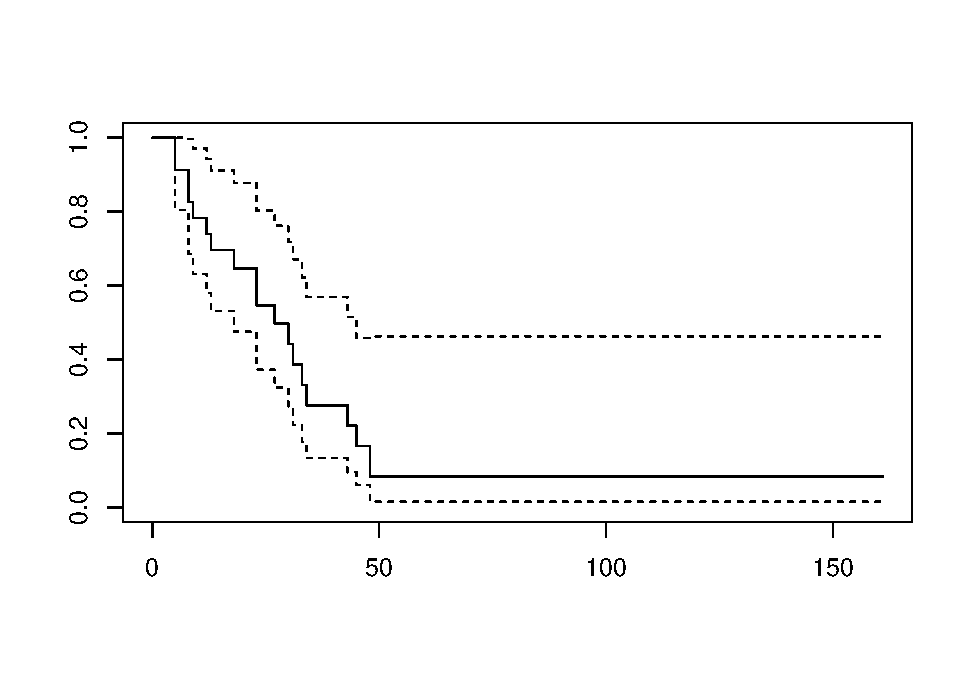
\includegraphics{07-week7_files/figure-latex/week7d-1.pdf}

Use ``\textasciitilde{} covariate'' instead of ``\textasciitilde{} 1'' to plot survival curves by group:

\begin{Shaded}
\begin{Highlighting}[]
\KeywordTok{plot}\NormalTok{(}\KeywordTok{survfit}\NormalTok{(example7a_surv }\OperatorTok{~}\StringTok{ }\NormalTok{drug, }\DataTypeTok{data =}\NormalTok{ example7a))}
\end{Highlighting}
\end{Shaded}

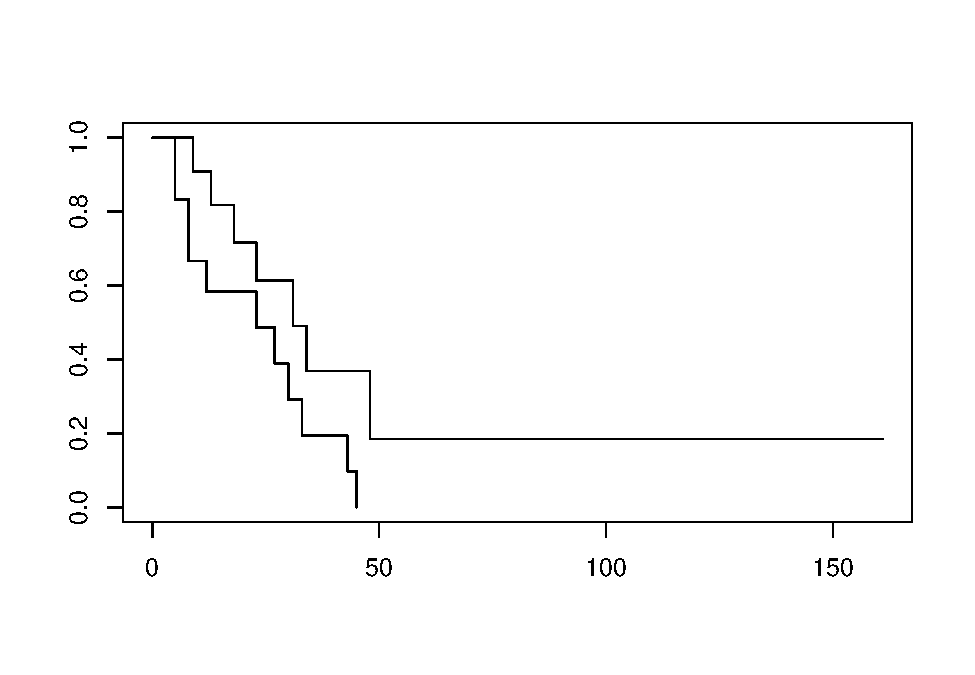
\includegraphics{07-week7_files/figure-latex/week7e-1.pdf}

Graphs can be saved out by using the ``Export'' option at the top of the ``Plots'' tab.

The \texttt{survdiff} function compares survival for different groups. For example, the following code compares survival for each value of the variable ``drug'' (generally 0 and 1).

\begin{Shaded}
\begin{Highlighting}[]
\KeywordTok{survdiff}\NormalTok{(example7a_surv }\OperatorTok{~}\StringTok{ }\NormalTok{drug, }\DataTypeTok{data =}\NormalTok{ example7a)}
\end{Highlighting}
\end{Shaded}

\begin{verbatim}
## Call:
## survdiff(formula = example7a_surv ~ drug, data = example7a)
## 
##         N Observed Expected (O-E)^2/E (O-E)^2/V
## drug=0 12       11     7.31      1.86       3.4
## drug=1 11        7    10.69      1.27       3.4
## 
##  Chisq= 3.4  on 1 degrees of freedom, p= 0.07
\end{verbatim}

The \texttt{coxph} function (from \texttt{survival}) is for regression analyses. For example, a unvariate regression for the effects of ``drug'' on survival:

\begin{Shaded}
\begin{Highlighting}[]
\KeywordTok{coxph}\NormalTok{(example7a_surv }\OperatorTok{~}\StringTok{ }\NormalTok{drug, }\DataTypeTok{data =}\NormalTok{ example7a)}
\end{Highlighting}
\end{Shaded}

\begin{verbatim}
## Call:
## coxph(formula = example7a_surv ~ drug, data = example7a)
## 
##         coef exp(coef) se(coef)      z      p
## drug -0.9155    0.4003   0.5119 -1.788 0.0737
## 
## Likelihood ratio test=3.38  on 1 df, p=0.06581
## n= 23, number of events= 18
\end{verbatim}

\begin{Shaded}
\begin{Highlighting}[]
\CommentTok{#You can use the tbl_regression function with Cox models to see the hazard ratios}
\NormalTok{example7a_cox <-}\StringTok{ }\KeywordTok{coxph}\NormalTok{(example7a_surv }\OperatorTok{~}\StringTok{ }\NormalTok{drug, }\DataTypeTok{data =}\NormalTok{ example7a)}
\KeywordTok{tbl_regression}\NormalTok{(example7a_cox, }\DataTypeTok{exponentiate =} \OtherTok{TRUE}\NormalTok{)}
\end{Highlighting}
\end{Shaded}

\captionsetup[table]{labelformat=empty,skip=1pt}
\begin{longtable}{lccc}
\toprule
\textbf{N = 23} & \textbf{HR}\textsuperscript{1} & \textbf{95\% CI}\textsuperscript{1} & \textbf{p-value} \\ 
\midrule
drug & 0.40 & 0.15, 1.09 & 0.074 \\ 
\bottomrule
\end{longtable}
\vspace{-5mm}
\begin{minipage}{\linewidth}
\textsuperscript{1}HR = Hazard Ratio, CI = Confidence Interval \\ 
\end{minipage}

The following multivariable model also includes some demographic and medical characteristics:

\begin{Shaded}
\begin{Highlighting}[]
\KeywordTok{coxph}\NormalTok{(example7a_surv }\OperatorTok{~}\StringTok{ }\NormalTok{drug }\OperatorTok{+}\StringTok{ }\NormalTok{age }\OperatorTok{+}\StringTok{ }\NormalTok{sex }\OperatorTok{+}\StringTok{ }\NormalTok{marker, }\DataTypeTok{data =}\NormalTok{ example7a)}
\end{Highlighting}
\end{Shaded}

\begin{verbatim}
## Call:
## coxph(formula = example7a_surv ~ drug + age + sex + marker, data = example7a)
## 
##            coef exp(coef) se(coef)      z       p
## drug   -1.76118   0.17184  0.68158 -2.584 0.00977
## age     0.01378   1.01388  0.02377  0.580 0.56199
## sex     1.01668   2.76401  0.58228  1.746 0.08080
## marker -0.80492   0.44712  0.42618 -1.889 0.05893
## 
## Likelihood ratio test=8.79  on 4 df, p=0.06668
## n= 23, number of events= 18
\end{verbatim}

Using the \texttt{summary} function with \texttt{survfit} lists all available followup times along with survival probabilities (you get a 95\% C.I. as well):

\begin{Shaded}
\begin{Highlighting}[]
\CommentTok{# For the entire cohort}
\KeywordTok{summary}\NormalTok{(}\KeywordTok{survfit}\NormalTok{(example7a_surv }\OperatorTok{~}\StringTok{ }\DecValTok{1}\NormalTok{, }\DataTypeTok{data =}\NormalTok{ example7a))}
\end{Highlighting}
\end{Shaded}

\begin{verbatim}
## Call: survfit(formula = example7a_surv ~ 1, data = example7a)
## 
##  time n.risk n.event survival std.err lower 95% CI upper 95% CI
##     5     23       2   0.9130  0.0588       0.8049        1.000
##     8     21       2   0.8261  0.0790       0.6848        0.996
##     9     19       1   0.7826  0.0860       0.6310        0.971
##    12     18       1   0.7391  0.0916       0.5798        0.942
##    13     17       1   0.6957  0.0959       0.5309        0.912
##    18     14       1   0.6460  0.1011       0.4753        0.878
##    23     13       2   0.5466  0.1073       0.3721        0.803
##    27     11       1   0.4969  0.1084       0.3240        0.762
##    30      9       1   0.4417  0.1095       0.2717        0.718
##    31      8       1   0.3865  0.1089       0.2225        0.671
##    33      7       1   0.3313  0.1064       0.1765        0.622
##    34      6       1   0.2761  0.1020       0.1338        0.569
##    43      5       1   0.2208  0.0954       0.0947        0.515
##    45      4       1   0.1656  0.0860       0.0598        0.458
##    48      2       1   0.0828  0.0727       0.0148        0.462
\end{verbatim}

\begin{Shaded}
\begin{Highlighting}[]
\CommentTok{# You can also summarize the survival by group:}
\KeywordTok{summary}\NormalTok{(}\KeywordTok{survfit}\NormalTok{(example7a_surv }\OperatorTok{~}\StringTok{ }\NormalTok{drug, }\DataTypeTok{data =}\NormalTok{ example7a))}
\end{Highlighting}
\end{Shaded}

\begin{verbatim}
## Call: survfit(formula = example7a_surv ~ drug, data = example7a)
## 
##                 drug=0 
##  time n.risk n.event survival std.err lower 95% CI upper 95% CI
##     5     12       2   0.8333  0.1076       0.6470        1.000
##     8     10       2   0.6667  0.1361       0.4468        0.995
##    12      8       1   0.5833  0.1423       0.3616        0.941
##    23      6       1   0.4861  0.1481       0.2675        0.883
##    27      5       1   0.3889  0.1470       0.1854        0.816
##    30      4       1   0.2917  0.1387       0.1148        0.741
##    33      3       1   0.1944  0.1219       0.0569        0.664
##    43      2       1   0.0972  0.0919       0.0153        0.620
##    45      1       1   0.0000     NaN           NA           NA
## 
##                 drug=1 
##  time n.risk n.event survival std.err lower 95% CI upper 95% CI
##     9     11       1    0.909  0.0867       0.7541        1.000
##    13     10       1    0.818  0.1163       0.6192        1.000
##    18      8       1    0.716  0.1397       0.4884        1.000
##    23      7       1    0.614  0.1526       0.3769        0.999
##    31      5       1    0.491  0.1642       0.2549        0.946
##    34      4       1    0.368  0.1627       0.1549        0.875
##    48      2       1    0.184  0.1535       0.0359        0.944
\end{verbatim}

The \texttt{times} option allows you to get survival probabilities for specific timepoints. For example, at 1 year, 2 years and 5 years:

\begin{Shaded}
\begin{Highlighting}[]
\KeywordTok{summary}\NormalTok{(}\KeywordTok{survfit}\NormalTok{(example7a_surv }\OperatorTok{~}\StringTok{ }\DecValTok{1}\NormalTok{, }\DataTypeTok{data =}\NormalTok{ example7a), }\DataTypeTok{times =} \KeywordTok{c}\NormalTok{(}\DecValTok{12}\NormalTok{, }\DecValTok{24}\NormalTok{, }\DecValTok{60}\NormalTok{))}
\end{Highlighting}
\end{Shaded}

\begin{verbatim}
## Call: survfit(formula = example7a_surv ~ 1, data = example7a)
## 
##  time n.risk n.event survival std.err lower 95% CI upper 95% CI
##    12     18       6   0.7391  0.0916       0.5798        0.942
##    24     11       4   0.5466  0.1073       0.3721        0.803
##    60      1       8   0.0828  0.0727       0.0148        0.462
\end{verbatim}

\begin{Shaded}
\begin{Highlighting}[]
\CommentTok{# "t" is in months}
\end{Highlighting}
\end{Shaded}

So, some typical code to analyze a data set:

\begin{Shaded}
\begin{Highlighting}[]
\CommentTok{# Create your survival object, which indicates this is a time to event outcome}
\NormalTok{example7a_surv <-}\StringTok{ }\KeywordTok{Surv}\NormalTok{(example7a}\OperatorTok{$}\NormalTok{t, example7a}\OperatorTok{$}\NormalTok{d)}

\CommentTok{# Get median survival and number of events for group}
\KeywordTok{survfit}\NormalTok{(example7a_surv }\OperatorTok{~}\StringTok{ }\DecValTok{1}\NormalTok{)}
\end{Highlighting}
\end{Shaded}

\begin{verbatim}
## Call: survfit(formula = example7a_surv ~ 1)
## 
##       n  events  median 0.95LCL 0.95UCL 
##      23      18      27      18      45
\end{verbatim}

\begin{Shaded}
\begin{Highlighting}[]
\CommentTok{# Get median followup for survivors}
\NormalTok{example7a }\OperatorTok
\StringTok{  }\KeywordTok{filter}\NormalTok{(d }\OperatorTok{==}\StringTok{ }\DecValTok{0}\NormalTok{) }\OperatorTok
\StringTok{  }\KeywordTok{skim}\NormalTok{(t)}
\end{Highlighting}
\end{Shaded}

\begin{verbatim}
## Skim summary statistics
##  n obs: 5 
##  n variables: 6 
## 
## -- Variable type:numeric ---------------------------------------------------------------
##  variable missing complete n mean    sd p0 p25 p50 p75 p100     hist
##         t       0        5 5 52.6 61.89 13  16  28  45  161 ▇▂▁▁▁▁▁▂
\end{verbatim}

\begin{Shaded}
\begin{Highlighting}[]
\CommentTok{# Show a graph}
\KeywordTok{plot}\NormalTok{(}\KeywordTok{survfit}\NormalTok{(example7a_surv }\OperatorTok{~}\StringTok{ }\DecValTok{1}\NormalTok{))}
\end{Highlighting}
\end{Shaded}

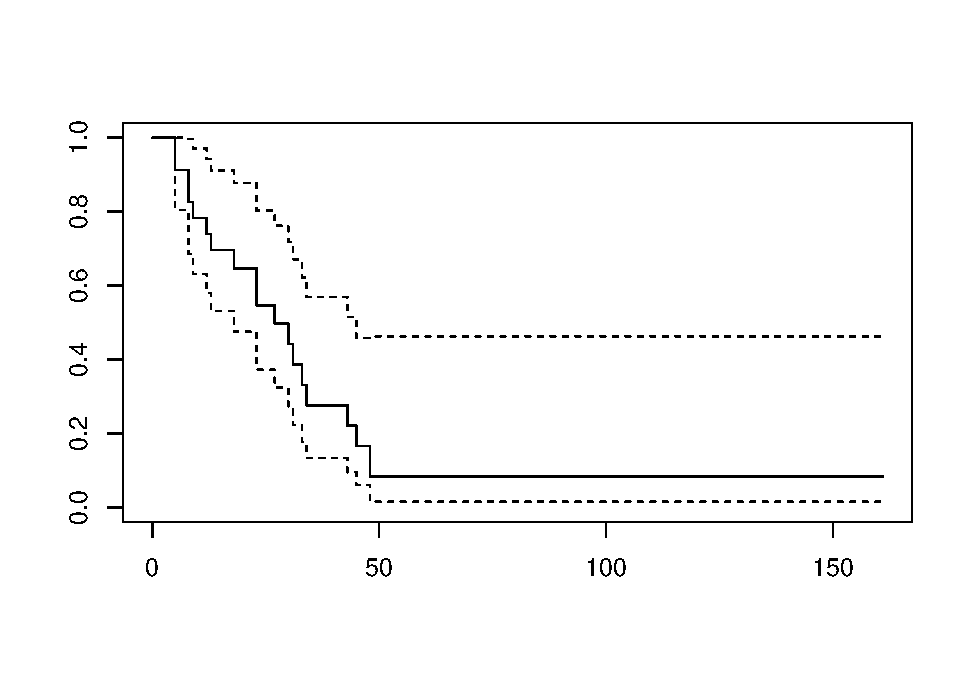
\includegraphics{07-week7_files/figure-latex/week7k-1.pdf}

\begin{Shaded}
\begin{Highlighting}[]
\CommentTok{# Look at predictors of survival}
\KeywordTok{coxph}\NormalTok{(example7a_surv }\OperatorTok{~}\StringTok{ }\NormalTok{drug }\OperatorTok{+}\StringTok{ }\NormalTok{age }\OperatorTok{+}\StringTok{ }\NormalTok{sex }\OperatorTok{+}\StringTok{ }\NormalTok{marker, }\DataTypeTok{data =}\NormalTok{ example7a)}
\end{Highlighting}
\end{Shaded}

\begin{verbatim}
## Call:
## coxph(formula = example7a_surv ~ drug + age + sex + marker, data = example7a)
## 
##            coef exp(coef) se(coef)      z       p
## drug   -1.76118   0.17184  0.68158 -2.584 0.00977
## age     0.01378   1.01388  0.02377  0.580 0.56199
## sex     1.01668   2.76401  0.58228  1.746 0.08080
## marker -0.80492   0.44712  0.42618 -1.889 0.05893
## 
## Likelihood ratio test=8.79  on 4 df, p=0.06668
## n= 23, number of events= 18
\end{verbatim}

\hypertarget{assignments-6}{%
\section{Assignments}\label{assignments-6}}

Try to do at least lesson7a and lesson7b

\begin{itemize}
\item
  lesson7a.rds: This is a large set of data on patients receiving adjuvant therapy after surgery for colon cancer. Describe this data set and determine which, if any, variables are prognostic in this patient group.
\item
  lesson7b.rds: These are time to recurrence data on forty patients with biliary cancer treated at one of two hospitals, one of which treats a large number of cancer patients and one of which does not. Do patients treated at a ``high volume'' hospital have a longer time to recurrence?
\item
  lesson7c.rds: These are data from a randomized trial comparing no treatment, levamisole (an immune stimulant) and levamisole combined with 5FU (a chemotherapy agent) and in the adjuvant treatment of colon cancer. Describe the data set. What conclusions would you draw about the effectiveness of the different treatments?
\item
  lesson7d.rds: More data on time to recurrence by hospital volume. Given this data set, determine whether patients treated at a ``high volume'' hospital have a longer time to recurrence.
\end{itemize}

\hypertarget{week-8}{%
\chapter{Week 8}\label{week-8}}

Statistical Slipups Powerpoint Presentation

{[}{[}TODO: Add link after pushed to Github{]}{]}

\hypertarget{assignment-answers}{%
\chapter{Assignment Answers}\label{assignment-answers}}

\hypertarget{week-1-1}{%
\section{Week 1}\label{week-1-1}}

\textbf{This is data for 386 patients undergoing surgery. What type of data (e.g.~continuous, binary, ordinal, nonsense) are each of the variables?}

The data set has 11 variables:

\begin{itemize}
\tightlist
\item
  ``id'' is clearly a hospital record number. It doesn't matter what type of variable it is, because you only want to know the type of variable in order to summarize or analyze data, and you'd never want to analyze or summarize patient id.
\item
  ``sex'' is a binary variable
\item
  ``age'' is continuous
\item
  ``p1'', ``p2'', ``p3'', ``p4'' are the pain scores after surgery. They only take integer values between 0 and 6. They would therefore typically regarded as categorical, and because they are clearly ordered (i.e.~pain score of 6 is higher than one of 4) these variables can be described are ordinal. However, many statisticians, myself included, would think it perfectly reasonable to treat these variables as continuous.
\item
  ``t'': total pain score takes on values between 0 and 24 and can thus be considered continuous
\item
  ``x'', ``y'' and ``z'': should you attempt to summarize a variable if you don't know what it is? It is obvious for y, this is some kind of hospital location, and is a categorical variable. But what about x and z? As it happens, z looks ordinal but isn't: it is blood group coded 1=o, 2=a, 3=b, 4=ab.
\end{itemize}

\hypertarget{week-2-1}{%
\section{Week 2}\label{week-2-1}}

\hypertarget{lesson2a.rds-marathon-runners}{%
\subsection{lesson2a.rds: Marathon Runners}\label{lesson2a.rds-marathon-runners}}

\textbf{This is data from marathon runners: summarize age, sex, race time in minutes (i.e.~how long it took them to complete the race) and favorite running shoe.}

Age is continuous and normally distributed (look at a graph or look at the centiles) and so it wouldn't be unreasonable to describe age in terms of mean and standard deviation (SD) by using \texttt{lesson2a\ \%\textgreater{}\%\ skim(age)}: mean (42 years), SD of 10.2. By the way, don't just copy the readout from R: this would give mean age as 42.43 and implies we are interested in age within a few days.

Sex is binary: use \texttt{tbl\_summary(lesson2a\ \%\textgreater{}\%\ select(sex))} to get percentages. But note that the person who prepared the data didn't state how the variable was coded (someone with sex=1 is a woman or a man?). Now what you should do in this situation is ask, but here is another alternative:

\begin{Shaded}
\begin{Highlighting}[]
\NormalTok{lesson2a }\OperatorTok
\StringTok{  }\KeywordTok{group_by}\NormalTok{(sex) }\OperatorTok
\StringTok{  }\KeywordTok{skim}\NormalTok{(rt)}
\end{Highlighting}
\end{Shaded}

\begin{verbatim}
## Skim summary statistics
##  n obs: 98 
##  n variables: 6 
##  group variables: sex 
## 
## -- Variable type:numeric ---------------------------------------------------------------
##  sex variable missing complete  n   mean    sd  p0    p25   p50    p75
##    0       rt       0       66 66 243.23 49.85 158 214.25 236   268.75
##    1       rt       0       32 32 264.84 37.45 222 237    251.5 283.25
##  p100     hist
##   414 ▅▇▇▆▃▂▁▁
##   362 ▇▅▅▂▁▂▂▁
\end{verbatim}

So sex==0 are running faster than the sex==1 and it would not be unreasonable to assume that sex==1 means women.

Race time is continuous and looks pretty normal. Yes the data are skewed by a single outlier (a race time of 414 minutes) but the mean and median are pretty similar (250 v. 242 minutes) and the 5th and 95th centile are very close to the values expected by adding or subtracting 1.64 times the SD from the mean (5th centile is 176, expected value using means and SD is 173; 95th centile actual and expected values are 328 and 328). I would probably feel comfortable reporting a mean and SD if you wanted.

Favorite running shoe: \texttt{lesson2a\ \%\textgreater{}\%\ skim(shoe)} gives a mean of 3.08 and a median of 3. If you reported these, you need therapy: shoe is a categorical variable and you should report the percentage of runners that favor each shoe.

AN ADDITIONAL IMPORTANT POINT: you should give the number of observations and the number of missing observations. n is 98 for all observations except for favorite running shoe, where there are 95 observations and 3 missing observations.

So here is a model answer, suitable for publication (assuming that sex==1 is coded as female.)

\captionsetup[table]{labelformat=empty,skip=1pt}
\begin{longtable}{lc}
\toprule
\textbf{Characteristic}\textsuperscript{1} & \textbf{N = 98} \\ 
\midrule
Age & 42 (10)) \\ 
Women & 32 (33\%) \\ 
Race time in minutes & 250 (47)) \\ 
Favorite Running Shoe &  \\ 
Asics & 14 (15\%) \\ 
New Balance & 7 (7.4\%) \\ 
Nike & 31 (33\%) \\ 
Saucony & 43 (45\%) \\ 
Unknown & 3 \\ 
\bottomrule
\end{longtable}
\vspace{-5mm}
\begin{minipage}{\linewidth}
\textsuperscript{1}Statistics presented: mean (SD)); n (\%) \\ 
\end{minipage}

However, look at this.

\captionsetup[table]{labelformat=empty,skip=1pt}
\begin{longtable}{lc}
\toprule
\textbf{Characteristic}\textsuperscript{1} & \textbf{N = 98} \\ 
\midrule
Age & 43 (34, 48) \\ 
Women & 32 (33\%) \\ 
Race time in minutes & 242 (222, 273) \\ 
Favorite Running Shoe &  \\ 
Asics & 14 (15\%) \\ 
New Balance & 7 (7.4\%) \\ 
Nike & 31 (33\%) \\ 
Saucony & 43 (45\%) \\ 
Unknown & 3 \\ 
\bottomrule
\end{longtable}
\vspace{-5mm}
\begin{minipage}{\linewidth}
\textsuperscript{1}Statistics presented: median (IQR); n (\%) \\ 
\end{minipage}

This really isn't much to distinguish between these tables. On the one hand using the mean and SD gives you more information (e.g.~what proportion of patients are aged over 70?). On the other hand, I can't see anyone using a table 1 to do these types of calculation and the median and interquartile range give you some more immediately usable information (no multiplying by 1.64!).

\hypertarget{lesson2b.rds-postoperative-pain}{%
\subsection{lesson2b.rds: Postoperative Pain}\label{lesson2b.rds-postoperative-pain}}

\textbf{Summarize average pain after the operation. Imagine you had to draw a graph of ``time course of pain after surgery''. What numbers would you use for pain at time 1, time 2, time 3, etc.?}

This is data on postoperative pain. You were asked to summarize average pain after the operation. This is continuous, so by looking at the histogram, you can see that the data look skewed. I would be tempted to use the median (1.8) and quartiles (1.1, 2.6).

\begin{Shaded}
\begin{Highlighting}[]
\KeywordTok{ggplot}\NormalTok{(}\DataTypeTok{data =}\NormalTok{ lesson2b,}
       \KeywordTok{aes}\NormalTok{(}\DataTypeTok{x =}\NormalTok{ t)) }\OperatorTok{+}
\StringTok{  }\KeywordTok{geom_histogram}\NormalTok{()}
\end{Highlighting}
\end{Shaded}

\begin{verbatim}
## `stat_bin()` using `bins = 30`. Pick better value with `binwidth`.
\end{verbatim}

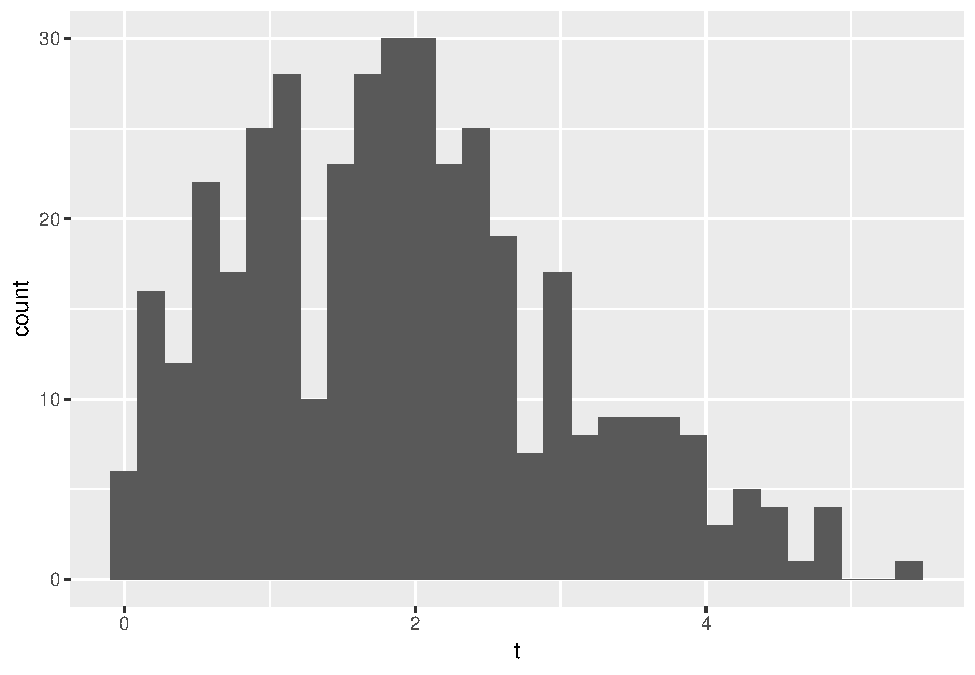
\includegraphics{09-answers_files/figure-latex/week2d-1.pdf}

However, using the mean and standard deviation doesn't get you far off. For normal data, 50\% of the observations are within two-thirds of a standard deviations of the mean. So the interquartile range predicted from the mean and SD would be 1.9 - 1.1*0.67 and 1.9 + 1.1*0.67 which gives you 1.2 and 2.7. This is an interesting point: the data can look skewed (and if you are interested, a statistical test can tell you that the data are definitely non-normal) but it doesn't make much of a difference in practice.

You were then asked to imagine that you had to draw a graph of ``time course of pain after surgery''. What numbers would you use for time 1, time 2 etc? The first thing to note is that to draw the graph, which seems like a useful thing to do, you have to treat the data as continuous: you can't really graph a table very easily. This is another illustration of how something that seems technically incorrect gives you useful approximations. Now that we have continuous data we have to decide whether to use medians or means. As it turns out, normality of the data isn't even an issue. Here is what happens if you graph the median pain score at each time point.

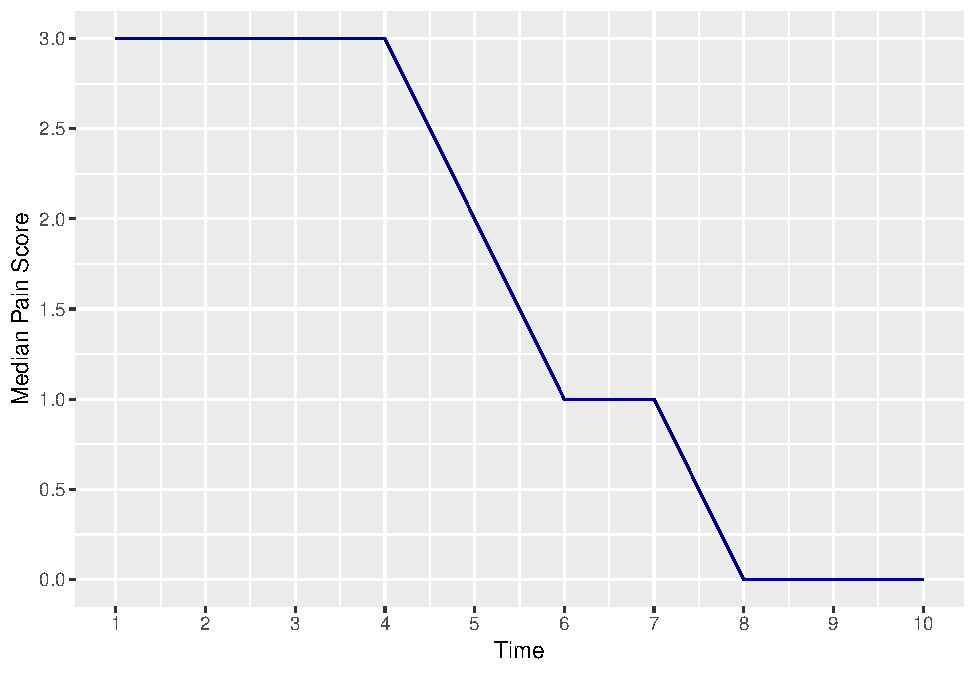
\includegraphics{09-answers_files/figure-latex/week2e-1.pdf}

This makes it seem that postoperative pain doesn't change for four time points, then drops dramatically.

A graph using means seems more illustrative of what is really going on.

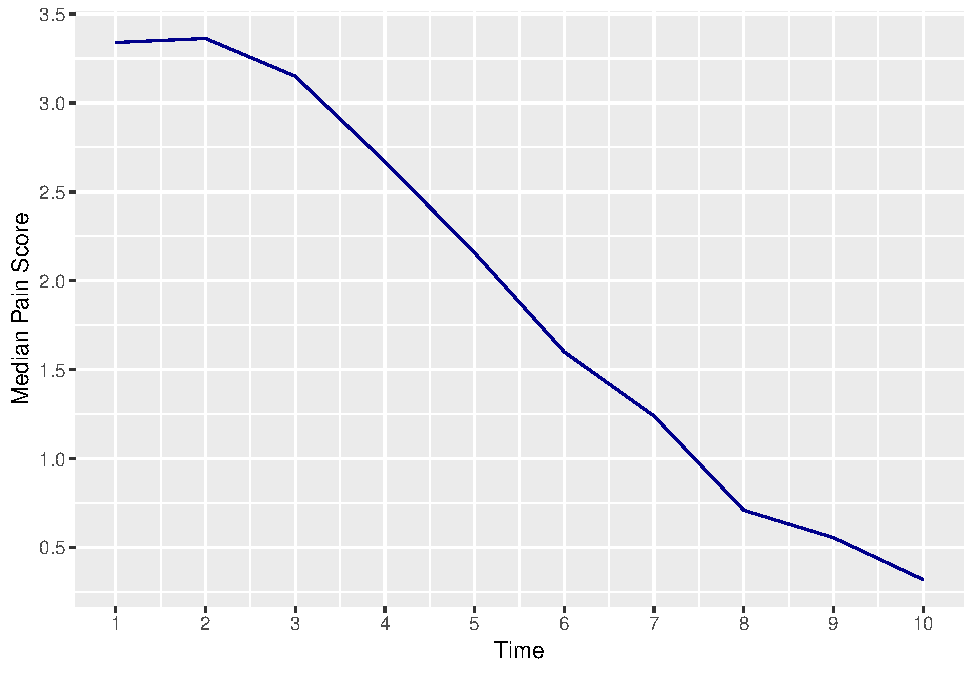
\includegraphics{09-answers_files/figure-latex/week2f-1.pdf}

\hypertarget{lesson2c.rds-radical-prostatectomy-cohort}{%
\subsection{lesson2c.rds: Radical Prostatectomy Cohort}\label{lesson2c.rds-radical-prostatectomy-cohort}}

\textbf{This is data on 242 patients undergoing radical prostatectomy. Summarize age, stage, grade and PSA.}

One of the first things to look for here is missing data. If you type \texttt{lesson2c\ \%\textgreater{}\%\ skim()}, you'll see that there is no missing data for age, 9 missing observations for PSA and 41 for grade. You will notice that the ``stage'' variable is not included here, because it is a character variable, not a numeric variable.

If you type \texttt{tbl\_summary(lesson2c\ \%\textgreater{}\%\ select(stage))}, you'll see that all patients have a stage assigned (no ``NA'' values).

A second issue is how to characterize the categorical variables. There are 8 different stages represented, many with very small numbers (like 2 for T4 and T1B, 4 for T3). It generally isn't very helpful to slice and dice data into very small categories, so I would consider grouping. For instance, we could group the T1s and T3 and 4 to get something like:

\captionsetup[table]{labelformat=empty,skip=1pt}
\begin{longtable}{lc}
\toprule
\textbf{Characteristic}\textsuperscript{1} & \textbf{N = 241} \\ 
\midrule
Stage &  \\ 
T1 & 169 (70\%) \\ 
T2A & 36 (15\%) \\ 
T2B & 22 (9.1\%) \\ 
T2C & 8 (3.3\%) \\ 
T3/4 & 6 (2.5\%) \\ 
\bottomrule
\end{longtable}
\vspace{-5mm}
\begin{minipage}{\linewidth}
\textsuperscript{1}Statistics presented: n (\%) \\ 
\end{minipage}

To get the table, I created a new variable as follows:

\begin{Shaded}
\begin{Highlighting}[]
\NormalTok{lesson2c <-}
\StringTok{  }\NormalTok{lesson2c }\OperatorTok
\StringTok{  }\KeywordTok{mutate}\NormalTok{(}
    \DataTypeTok{stage_category =}
      \KeywordTok{case_when}\NormalTok{(}
\NormalTok{        stage }\OperatorTok\StringTok{ }\KeywordTok{c}\NormalTok{(}\StringTok{"T1A"}\NormalTok{, }\StringTok{"T1B"}\NormalTok{, }\StringTok{"T1C"}\NormalTok{) }\OperatorTok{~}\StringTok{ "T1"}\NormalTok{,}
\NormalTok{        stage }\OperatorTok\StringTok{ }\KeywordTok{c}\NormalTok{(}\StringTok{"T3"}\NormalTok{, }\StringTok{"T4"}\NormalTok{) }\OperatorTok{~}\StringTok{ "T3/4"}\NormalTok{,}
        \OtherTok{TRUE} \OperatorTok{~}\StringTok{ }\NormalTok{stage}
\NormalTok{      )}
\NormalTok{  )}
\end{Highlighting}
\end{Shaded}

The \texttt{case\_when} function is similar to the \texttt{if\_else} function, but it allows for more than the 2 options of TRUE/FALSE. In this case, TRUE indicates all values that were not included in the prior categories.

There is a similar issue for grade, with few patients having grades 4, 5, 8 or 9. Now a key point is that what you decide to do in situations like this will often need to take into account your medical understanding. It might seems sensible to categorize grade as ≤6 or ≥7, or perhaps 4/5, 6, 7, 8/9. But as it turns out in prostate cancer, pathologists can't reliably grade a cancer as 4 or 5 and these cancers should really be grouped with grade 6. Grade 8, on the other hand, signifies very aggressive disease and really needs to be reported separately even if there are only a few patients with grade 8. So grade would probably be summarized as per the following table:

\captionsetup[table]{labelformat=empty,skip=1pt}
\begin{longtable}{lc}
\toprule
\textbf{Characteristic}\textsuperscript{1} & \textbf{N = 241} \\ 
\midrule
Stage &  \\ 
T1 & 169 (70\%) \\ 
T2A & 36 (15\%) \\ 
T2B & 22 (9.1\%) \\ 
T2C & 8 (3.3\%) \\ 
T3/4 & 6 (2.5\%) \\ 
Grade &  \\ 
6 & 79 (40\%) \\ 
7 & 112 (56\%) \\ 
8 & 9 (4.5\%) \\ 
Unknown & 41 \\ 
Age & 60 (56, 65) \\ 
PSA & 5.3 (4.0, 8.0) \\ 
Unknown & 9 \\ 
\bottomrule
\end{longtable}
\vspace{-5mm}
\begin{minipage}{\linewidth}
\textsuperscript{1}Statistics presented: n (\%); median (IQR) \\ 
\end{minipage}

\hypertarget{lesson2d.rds-cost-of-a-minor-medical-procedure}{%
\subsection{lesson2d.rds: Cost of a Minor Medical Procedure}\label{lesson2d.rds-cost-of-a-minor-medical-procedure}}

\textbf{Summarize cost.}

I asked you to summarize the cost. You can see from a graph that the data are not normally distributed. If we were to follow the rule book slavishly, we would report a median and interquartile range. But what use is a median for cost data? We want to know ``average'' cost so that we can predict, for example, how much we should budget for next year. This requires a mean.

\hypertarget{lesson2e.rds-cancer-pain}{%
\subsection{lesson2e.rds: Cancer pain}\label{lesson2e.rds-cancer-pain}}

\textbf{Summarize total cancer pain in one month in a group of chronic cancer patients.}

The data are grossly non-normal and you could use the median pain score with interquartile range.

As for summarizing the number of days in pain, almost everyone has 31 days of pain. So I would give proportions of patients who had pain for 31 days and then the number who, say, had pain at least 3 out of every 4 days and 2 out of 4 days. There are two ways of doing this. You could use \texttt{tbl\_summary(lesson2e\ \%\textgreater{}\%\ select(f),\ type\ =\ list(f\ =\ "categorical"))} and then combine some of the results. Or, and this is a little more complicated, you could create a new variable.

\begin{Shaded}
\begin{Highlighting}[]
\NormalTok{lesson2e <-}
\StringTok{  }\NormalTok{lesson2e }\OperatorTok
\StringTok{  }\KeywordTok{mutate}\NormalTok{(}
    \DataTypeTok{days =}
      \KeywordTok{case_when}\NormalTok{(}
\NormalTok{        f }\OperatorTok{<=}\StringTok{ }\DecValTok{15} \OperatorTok{~}\StringTok{ }\DecValTok{0}\NormalTok{,}
\NormalTok{        f }\OperatorTok{>}\StringTok{ }\DecValTok{15} \OperatorTok{&}\StringTok{ }\NormalTok{f }\OperatorTok{<}\StringTok{ }\DecValTok{23} \OperatorTok{~}\StringTok{ }\DecValTok{1}\NormalTok{,}
\NormalTok{        f }\OperatorTok{>}\StringTok{ }\DecValTok{23} \OperatorTok{&}\StringTok{ }\NormalTok{f }\OperatorTok{<}\StringTok{ }\DecValTok{31} \OperatorTok{~}\StringTok{ }\DecValTok{2}\NormalTok{,}
\NormalTok{        f }\OperatorTok{==}\StringTok{ }\DecValTok{31} \OperatorTok{~}\StringTok{ }\DecValTok{3}
\NormalTok{      )}
\NormalTok{  )}
\end{Highlighting}
\end{Shaded}

In other words, create a new variable called ``days'', and set it to 0 for anyone with 15 or less days of pain. Call anyone who has pain more than half the time (i.e.~more than 15 days) a 1. Call anyone who has pain more than three quarter of the time (i.e.~more than 23 days) a 2. Call anyone who has pain all the time a 3.

\begin{Shaded}
\begin{Highlighting}[]
\KeywordTok{tbl_summary}\NormalTok{(}
\NormalTok{  lesson2e }\OperatorTok\StringTok{ }\KeywordTok{select}\NormalTok{(days)}
\NormalTok{)}
\end{Highlighting}
\end{Shaded}

\captionsetup[table]{labelformat=empty,skip=1pt}
\begin{longtable}{lc}
\toprule
\textbf{Characteristic}\textsuperscript{1} & \textbf{N = 100} \\ 
\midrule
days &  \\ 
0 & 16 (17\%) \\ 
1 & 7 (7.4\%) \\ 
2 & 23 (24\%) \\ 
3 & 48 (51\%) \\ 
Unknown & 6 \\ 
\bottomrule
\end{longtable}
\vspace{-5mm}
\begin{minipage}{\linewidth}
\textsuperscript{1}Statistics presented: n (\%) \\ 
\end{minipage}

So you could report that, of the 94 patients with data on number of days with pain, 51\% were in daily pain, 17\% of patients had pain on less than half of days, 7.4\% of patients had pain on more than half but less than 75\% of days, 24\% of patients had pain on more than 75\% of days, but not every day.

\emph{For keen students only!}

You could also try a log transformation of the pain scores. Create a new variable using \texttt{log(pain)}.

\begin{Shaded}
\begin{Highlighting}[]
\NormalTok{lesson2e <-}
\StringTok{  }\NormalTok{lesson2e }\OperatorTok
\StringTok{  }\KeywordTok{mutate}\NormalTok{(}\DataTypeTok{log =} \KeywordTok{log}\NormalTok{(pain))}
\end{Highlighting}
\end{Shaded}

Analyze this variable and you'll see it appears normally distributed.

The mean of log is 5.42. You can transform the log back by calculating e\textsuperscript{5.42} (the function is \texttt{exp(5.42)}) to get 225, close to the median. Backtransforming the standard deviation is more complicated and can't really be done directly. What you need to do is make any calculations you need on the log transformed scale and then backtransform the results. Imagine you wanted a 95\% confidence interval. A 95\% confidence interval is the mean ± 1.96 standard deviations. The standard deviation of the log data is close to one. So the confidence interval is 3.45 to 7.39. Transforming this \texttt{exp(3.45)} and \texttt{exp(7.39)} gives a confidence interval on the original scale of 31.44 and 1614.07. This is a reasonable approximation to the 5th (50) and 95th centile (1319).

\hypertarget{week-3-1}{%
\section{Week 3}\label{week-3-1}}

\hypertarget{lesson3a.rds}{%
\subsection{lesson3a.rds}\label{lesson3a.rds}}

\textbf{These are data from over 1000 patients undergoing chemotherapy reporting a nausea and vomiting score from 0 to 10. Does previous chemotherapy increase nausea scores? What about sex?}

Hands up, who typed in \texttt{t.test(nv\ \textasciitilde{}\ pc,\ data\ =\ lesson3a,\ var.equal\ =\ TRUE)} without looking at the data? There are lots of missing data. There is a question as to whether you would actually analyze these data at all: could data be missing because patients were too ill to complete questionnaires? Could there have been bias in ascertaining who had prior chemotherapy? If you do decide to analyze, a t-test would be appropriate (\texttt{t.test(nv\ \textasciitilde{}\ pc,\ data\ =\ lesson3a,\ var.equal\ =\ TRUE)} and \texttt{t.test(nv\ \textasciitilde{}\ sex,\ data\ =\ lesson3a,\ var.equal\ =\ TRUE)}). A model answer might be:

\begin{quote}
Details of prior chemotherapy were available for 512 of the 1098 patients with nausea scores. Mean nausea scores were approximately 20\% higher in the 255 patients with prior experience of chemotherapy (5.3; SD 2.03) than in the 257 chemotherapy-naive patients (4.5; SD 1.99). The difference between groups was small (0.8, 95\% C.I. 0.5, 1.2 but highly statistically significant (p\textless0.001 by t-test), suggesting that prior chemotherapy increases nausea scores. Nausea scores were slightly lower in women (n=444; mean 4.7; SD 1.98) than men (n=434; mean 4.8; SD 2.1) but there were no statistically significant differences between the sexes (difference between means 0.1, 95\% C.I. -0.2, 0.3); p=0.7 by t-test). However, far more women (131 / 575, 60\%) than men (89 / 523, 40\%) failed provide a nausea score (p=0.017 by chi squared), perhaps suggesting bias in reporting.
\end{quote}

Now, I'll explain what I did. First, I did the two t-tests:

\begin{Shaded}
\begin{Highlighting}[]
\KeywordTok{t.test}\NormalTok{(nv }\OperatorTok{~}\StringTok{ }\NormalTok{pc, }\DataTypeTok{data =}\NormalTok{ lesson3a, }\DataTypeTok{var.equal =} \OtherTok{TRUE}\NormalTok{)}
\end{Highlighting}
\end{Shaded}

\begin{verbatim}
## 
##  Two Sample t-test
## 
## data:  nv by pc
## t = -4.6275, df = 510, p-value = 4.7e-06
## alternative hypothesis: true difference in means is not equal to 0
## 95 percent confidence interval:
##  -1.1699123 -0.4725841
## sample estimates:
## mean in group 0 mean in group 1 
##        4.459144        5.280392
\end{verbatim}

\begin{Shaded}
\begin{Highlighting}[]
\KeywordTok{t.test}\NormalTok{(nv }\OperatorTok{~}\StringTok{ }\NormalTok{sex, }\DataTypeTok{data =}\NormalTok{ lesson3a, }\DataTypeTok{var.equal =} \OtherTok{TRUE}\NormalTok{)}
\end{Highlighting}
\end{Shaded}

\begin{verbatim}
## 
##  Two Sample t-test
## 
## data:  nv by sex
## t = 0.43835, df = 876, p-value = 0.6612
## alternative hypothesis: true difference in means is not equal to 0
## 95 percent confidence interval:
##  -0.2100764  0.3308988
## sample estimates:
## mean in group 0 mean in group 1 
##        4.782258        4.721847
\end{verbatim}

Then I created a new variable for missing data on nausea and vomiting:

\begin{Shaded}
\begin{Highlighting}[]
\NormalTok{lesson3a <-}
\StringTok{  }\NormalTok{lesson3a }\OperatorTok
\StringTok{  }\KeywordTok{mutate}\NormalTok{(}
    \DataTypeTok{missing =}
      \KeywordTok{if_else}\NormalTok{(}\KeywordTok{is.na}\NormalTok{(nv), }\DecValTok{1}\NormalTok{, }\DecValTok{0}\NormalTok{)}
\NormalTok{  )}
\end{Highlighting}
\end{Shaded}

And then the table:

\begin{Shaded}
\begin{Highlighting}[]
\KeywordTok{tbl_summary}\NormalTok{(}
\NormalTok{  lesson3a }\OperatorTok\StringTok{ }\KeywordTok{select}\NormalTok{(missing, sex),}
  \DataTypeTok{by =} \StringTok{"sex"}\NormalTok{,}
  \DataTypeTok{type =} \KeywordTok{list}\NormalTok{(}\DataTypeTok{missing =} \StringTok{"categorical"}\NormalTok{)}
\NormalTok{)}
\end{Highlighting}
\end{Shaded}

\captionsetup[table]{labelformat=empty,skip=1pt}
\begin{longtable}{lcc}
\toprule
\textbf{Characteristic}\textsuperscript{1} & \textbf{0}, N = 523 & \textbf{1}, N = 575 \\ 
\midrule
missing &  &  \\ 
0 & 434 (83\%) & 444 (77\%) \\ 
1 & 89 (17\%) & 131 (23\%) \\ 
\bottomrule
\end{longtable}
\vspace{-5mm}
\begin{minipage}{\linewidth}
\textsuperscript{1}Statistics presented: n (\%) \\ 
\end{minipage}

If you got that far: wow! (also, forget the course, you don't need it). If you didn't get that far, don't feel bad about it, but try to get a handle on the thought process.

One other issue: the p value for the first t-test (previous chemotherapy) is given as ``p-value = 4.709e-06''. While this number is very close to 0, we cannot round to 0 - there is no such thing as a p value of 0 for any hypothesis worth testing (there is a small but finite chance of every possible result, even throwing 100,000 tails in a row on an unbiased coin.) So do not report ``p=0.0000''! You can round p values for reporting - for example, ``4.709e-06'' can be rounded to ``\textless0.0005''.

\emph{For more advanced students:}

The other thing you can do is to find out the precise p value from the t value (which is given above the p value: -4.6275). The function you need is \texttt{pt(t\ value,\ degrees\ of\ freedom)}. This will give you the p value for a one-sided test, so you must multiply by 2 to get the two-sided test p value.

\begin{Shaded}
\begin{Highlighting}[]
\KeywordTok{pt}\NormalTok{(}\OperatorTok{-}\FloatTok{4.6275}\NormalTok{, }\DecValTok{510}\NormalTok{)}\OperatorTok{*}\DecValTok{2}
\end{Highlighting}
\end{Shaded}

\begin{verbatim}
## [1] 4.699746e-06
\end{verbatim}

This p-value can also be read as 4.7 x 10\textsuperscript{-6}. An interesting question though: is it important whether p is \textless0.0005 or 4.7 x 10\textsuperscript{-6}?

What is ``degrees of freedom'' and how come it is 510? Think about it this way: You have a line of ten people outside your door. You know the mean age of this group. Each person comes in one-by-one, you try to guess their age and they tell you how old they actually are. As each person comes in, your guesses will get better and better (for example, if the first three people have ages less than the mean, you will guess the age of the fourth person as something above the mean). However, only when you have the ages of the first nine people will you be able to guess for sure the age of the next (and last) person. In other words, the ages of the first nine people are ``free'', the age of the last person is ``constrained''. So ``degrees of freedom'' is the sample size minus one. Little catch though: for an unpaired test (such a straight drug v. placebo trial), you have two different groups and two different means. You would therefore be able to predict the scores of two observations (the last patient in each group). Degrees of freedom in an unpaired test is therefore the total sample size minus two (or, put another way, the sample size in group a minus one plus the sample size in group b minus one.)

\hypertarget{lesson3b.rds}{%
\subsection{lesson3b.rds}\label{lesson3b.rds}}

\textbf{Patients with wrist osteoarthritis are randomized to a new drug or placebo. Pain is measured before and after treatment. Is the drug effective?}

The data look relatively normal and the most obvious thing to do would be to do:

\begin{Shaded}
\begin{Highlighting}[]
\KeywordTok{t.test}\NormalTok{(p }\OperatorTok{~}\StringTok{ }\NormalTok{g, }\DataTypeTok{data =}\NormalTok{ lesson3b, }\DataTypeTok{var.equal =} \OtherTok{TRUE}\NormalTok{)}
\end{Highlighting}
\end{Shaded}

\begin{verbatim}
## 
##  Two Sample t-test
## 
## data:  p by g
## t = 1.9731, df = 34, p-value = 0.05665
## alternative hypothesis: true difference in means is not equal to 0
## 95 percent confidence interval:
##  -0.01930642  1.30819531
## sample estimates:
## mean in group 0 mean in group 1 
##      0.55555555     -0.08888889
\end{verbatim}

This gives a p value of 0.057 and you might conclude that there is a ``trend'' towards statistical significance suggesting that the drug works. However, the t-test assumes that the data are independent. In the present case, this assumption does not hold: each patient contributes data from two wrists, and the pain scores from each wrist are correlated. There are several ways around the problem. The most obvious is to say: ``These data are not independent, I am not going to analyze them. Call in a statistician.''

However, if you are really keen, you could try the following:

You could analyze the data from each wrist separately by creating new variables as shown below (lines with \# are comments).

\begin{Shaded}
\begin{Highlighting}[]
\NormalTok{lesson3b <-}
\StringTok{  }\NormalTok{lesson3b }\OperatorTok
\StringTok{  }\CommentTok{# Create a new variable called "pright" equivalent to "p", the pain score for the right wrist (site 2) only}
\StringTok{  }\KeywordTok{mutate}\NormalTok{(}
    \DataTypeTok{pright =} \KeywordTok{case_when}\NormalTok{(site }\OperatorTok{==}\StringTok{ }\DecValTok{2} \OperatorTok{~}\StringTok{ }\NormalTok{p)}
    \CommentTok{# By default, any observations that do not fall into the specified conditions in the "case_when" statement will be set to missing (NA)}
\NormalTok{  ) }\OperatorTok
\StringTok{  }\CommentTok{# Create a new variable called "pleft" for pain scores for the left wrist}
\StringTok{  }\KeywordTok{mutate}\NormalTok{(}
    \DataTypeTok{pleft =} \KeywordTok{case_when}\NormalTok{(site }\OperatorTok{==}\StringTok{ }\DecValTok{1} \OperatorTok{~}\StringTok{ }\NormalTok{p)}
\NormalTok{  )}

\CommentTok{# t-test for pain in right and left wrists separately}
\KeywordTok{t.test}\NormalTok{(pright }\OperatorTok{~}\StringTok{ }\NormalTok{g, }\DataTypeTok{data =}\NormalTok{ lesson3b, }\DataTypeTok{var.equal =} \OtherTok{TRUE}\NormalTok{)}
\end{Highlighting}
\end{Shaded}

\begin{verbatim}
## 
##  Two Sample t-test
## 
## data:  pright by g
## t = 1.6818, df = 16, p-value = 0.112
## alternative hypothesis: true difference in means is not equal to 0
## 95 percent confidence interval:
##  -0.2055046  1.7832823
## sample estimates:
## mean in group 0 mean in group 1 
##       0.6555555      -0.1333333
\end{verbatim}

\begin{Shaded}
\begin{Highlighting}[]
\KeywordTok{t.test}\NormalTok{(pleft }\OperatorTok{~}\StringTok{ }\NormalTok{g, }\DataTypeTok{data =}\NormalTok{ lesson3b, }\DataTypeTok{var.equal =} \OtherTok{TRUE}\NormalTok{)}
\end{Highlighting}
\end{Shaded}

\begin{verbatim}
## 
##  Two Sample t-test
## 
## data:  pleft by g
## t = 1.0418, df = 16, p-value = 0.313
## alternative hypothesis: true difference in means is not equal to 0
## 95 percent confidence interval:
##  -0.5174209  1.5174209
## sample estimates:
## mean in group 0 mean in group 1 
##      0.45555555     -0.04444445
\end{verbatim}

\hypertarget{lesson3c.rds}{%
\subsection{lesson3c.rds}\label{lesson3c.rds}}

\textbf{Some postoperative pain data again. Is pain on day 2 different than pain on day 1? Is pain on day 3 different from pain on day 2?}

The most obvious issue here is that you are measuring the same patients on two occasions, so you are going to want a paired test. Should you do a paired t-test? Many statisticians would prefer a non-parametric method given that the data take only five different values and that the number of observations is small. The following command gives you the ``Wilcoxon signed rank test'':

\begin{Shaded}
\begin{Highlighting}[]
\KeywordTok{wilcox.test}\NormalTok{(lesson3c}\OperatorTok{$}\NormalTok{t1, lesson3c}\OperatorTok{$}\NormalTok{t2, }\DataTypeTok{correct =} \OtherTok{FALSE}\NormalTok{, }\DataTypeTok{exact =} \OtherTok{FALSE}\NormalTok{, }\DataTypeTok{paired =} \OtherTok{TRUE}\NormalTok{)}
\end{Highlighting}
\end{Shaded}

\begin{verbatim}
## 
##  Wilcoxon signed rank test
## 
## data:  lesson3c$t1 and lesson3c$t2
## V = 41.5, p-value = 0.1303
## alternative hypothesis: true location shift is not equal to 0
\end{verbatim}

(By the way: I know this because that is what it says on the read out: if you had asked me yesterday, I doubt I would have remembered the name of a non-parametric paired test, another reason to think in concepts rather than remembering statistical techniques). The p value you get is p=0.13. We cannot conclude that pain scores are different. But is that all we want to say? The number of patients is small, maybe we failed to spot a difference. So let's try a t-test:

\begin{Shaded}
\begin{Highlighting}[]
\KeywordTok{t.test}\NormalTok{(lesson3c}\OperatorTok{$}\NormalTok{t1, lesson3c}\OperatorTok{$}\NormalTok{t2, }\DataTypeTok{var.equal =} \OtherTok{TRUE}\NormalTok{, }\DataTypeTok{paired =} \OtherTok{TRUE}\NormalTok{)}
\end{Highlighting}
\end{Shaded}

\begin{verbatim}
## 
##  Paired t-test
## 
## data:  lesson3c$t1 and lesson3c$t2
## t = 1.5467, df = 21, p-value = 0.1369
## alternative hypothesis: true difference in means is not equal to 0
## 95 percent confidence interval:
##  -0.09395838  0.63941292
## sample estimates:
## mean of the differences 
##               0.2727273
\end{verbatim}

The p value you get (p=0.14) is very similar to the non-parametric method and you get a confidence interval for the difference between means of -0.09, 0.64. What I would conclude from this is that pain is unlikely to be worse on day 2 than day 1 but any decrease in pain is probably not important.

What about normality of the data? Doesn't that figure into whether you assess by t-test or non-parametric? Well if you type look at the distribution of t1 and t2, you find that neither are normally distributed. But a paired t-test does not depend on the assumption that each set of data in a pair is distributed but that the differences between pairs are normally distributed. So you would have to create a new variable and look at that:

\begin{Shaded}
\begin{Highlighting}[]
\NormalTok{lesson3c <-}
\StringTok{  }\NormalTok{lesson3c }\OperatorTok
\StringTok{  }\KeywordTok{mutate}\NormalTok{(}\DataTypeTok{delta12 =}\NormalTok{ t2 }\OperatorTok{-}\StringTok{ }\NormalTok{t1)}

\KeywordTok{skim}\NormalTok{(lesson3c}\OperatorTok{$}\NormalTok{delta12)}
\end{Highlighting}
\end{Shaded}

\begin{verbatim}
## 
## Skim summary statistics
## 
## -- Variable type:numeric ---------------------------------------------------------------
##          variable missing complete  n  mean   sd p0 p25 p50 p75 p100
##  lesson3c$delta12       0       22 22 -0.27 0.83 -2  -1   0   0    1
##      hist
##  ▁▁▃▁▁▇▁▂
\end{verbatim}

As it turns out, the distribution of differences between pain scores are normally distributed even though pain at time 2 does not have a normal distribution. In fact, this is almost always the case.

Now let's compare t2 and t3. Again, no significant difference. Does this mean that pain does not decrease after an operation? Of course, we know that pain does indeed get better. This illustrates two points: first, don't ask questions you know the answer to; second, asking lots of questions (is pain on day 2 better than on day 1?; is pain on day 3 better on day 2?) is not as good as just asking one question: does pain decrease over time? We'll discuss how to answer this question later on in the course.

\hypertarget{lesson3d.rds}{%
\subsection{lesson3d.rds}\label{lesson3d.rds}}

\textbf{This is a single-arm, uncontrolled study of acupuncture for patients with neck pain. Does acupuncture increase range of motion? Just as many men as women get neck pain. Can we say anything about the sample chosen for this trial with respect to gender? The mean age of patients with neck pain is 58.2 years. Is the trial population representative with respect to age?}

This is before and after data, so again you'll want a paired test. The data are continuous, so a paired t-test is an option (if you are worried about normality, do both the parametric and non-parametric test and compare the results.)

There are two ways of doing the t-test:

\begin{enumerate}
\def\labelenumi{\arabic{enumi})}
\tightlist
\item
  Test whether the baseline scores are different from the post-treatment scores:
\end{enumerate}

\begin{Shaded}
\begin{Highlighting}[]
\KeywordTok{t.test}\NormalTok{(lesson3d}\OperatorTok{$}\NormalTok{b, lesson3d}\OperatorTok{$}\NormalTok{a, }\DataTypeTok{var.equal =} \OtherTok{TRUE}\NormalTok{, }\DataTypeTok{paired =} \OtherTok{TRUE}\NormalTok{)}
\end{Highlighting}
\end{Shaded}

\begin{verbatim}
## 
##  Paired t-test
## 
## data:  lesson3d$b and lesson3d$a
## t = -4.4912, df = 33, p-value = 8.19e-05
## alternative hypothesis: true difference in means is not equal to 0
## 95 percent confidence interval:
##  -35.17110 -13.24067
## sample estimates:
## mean of the differences 
##               -24.20588
\end{verbatim}

\begin{enumerate}
\def\labelenumi{\arabic{enumi})}
\setcounter{enumi}{1}
\tightlist
\item
  Test whether the difference between scores is different from zero:
\end{enumerate}

\begin{Shaded}
\begin{Highlighting}[]
\KeywordTok{t.test}\NormalTok{(lesson3d}\OperatorTok{$}\NormalTok{d, }\DataTypeTok{mu =} \DecValTok{0}\NormalTok{)}
\end{Highlighting}
\end{Shaded}

\begin{verbatim}
## 
##  One Sample t-test
## 
## data:  lesson3d$d
## t = 4.4912, df = 33, p-value = 8.19e-05
## alternative hypothesis: true mean is not equal to 0
## 95 percent confidence interval:
##  13.24067 35.17110
## sample estimates:
## mean of x 
##  24.20588
\end{verbatim}

Both methods give you an identical p value of \textless0.001. But note, I didn't ask for the p value. I asked ``Does acupuncture increase range of motion?'' Given that this is an uncontrolled trial, it may be that range of motion has improved naturally over time. So in fact you can't answer the question about whether acupuncture increases range of motion from these data!

BTW: for those who are interested, acupuncture has been shown to improve neck pain and range of motion in a controlled trial, see: Irnich D, Behrens N, Gleditsch JM, Stör W, Schrieber MA, Schöps P, Vickers AJ, Beyer A. Immediate effects of dry needling and acupuncture at distant points in chronic neck pain: results of a randomized, double-blind, sham-controlled crossover trial. Pain 2002;99(1-2):83)

\begin{Shaded}
\begin{Highlighting}[]
\KeywordTok{binom.test}\NormalTok{(}\KeywordTok{sum}\NormalTok{(lesson3d}\OperatorTok{$}\NormalTok{sex), }\KeywordTok{nrow}\NormalTok{(lesson3d), }\DataTypeTok{p =} \FloatTok{0.5}\NormalTok{)}
\end{Highlighting}
\end{Shaded}

\begin{verbatim}
## 
##  Exact binomial test
## 
## data:  sum(lesson3d$sex) and nrow(lesson3d)
## number of successes = 9, number of trials = 34, p-value = 0.009041
## alternative hypothesis: true probability of success is not equal to 0.5
## 95 percent confidence interval:
##  0.1288174 0.4436154
## sample estimates:
## probability of success 
##              0.2647059
\end{verbatim}

Only about a quarter of the patients are women, and the binomial test gives a p value of 0.009, suggesting that men are over-represented in this trial. But is this important?

\begin{Shaded}
\begin{Highlighting}[]
\KeywordTok{t.test}\NormalTok{(lesson3d}\OperatorTok{$}\NormalTok{age, }\DataTypeTok{mu =} \FloatTok{58.2}\NormalTok{)}
\end{Highlighting}
\end{Shaded}

\begin{verbatim}
## 
##  One Sample t-test
## 
## data:  lesson3d$age
## t = -2.261, df = 33, p-value = 0.03048
## alternative hypothesis: true mean is not equal to 58.2
## 95 percent confidence interval:
##  46.30921 57.57315
## sample estimates:
## mean of x 
##  51.94118
\end{verbatim}

Similarly, this t-test for age gives a p value of 0.030, but I doubt anyone would call a mean age of 52 much different from a mean age of 58, so you'd probably want to say that, ok, the trial patients are younger than we might expect, but not by much.

\hypertarget{lesson3e.rds}{%
\subsection{lesson3e.rds}\label{lesson3e.rds}}

\textbf{These data are length of stay from two different hospitals. One of the hospitals uses a new chemotherapy regime that is said to reduce adverse events and therefore length of stay. Does the new regime decrease length of stay?}

Well, before running off and doing t-tests, let's have a look at the data:

\begin{Shaded}
\begin{Highlighting}[]
\NormalTok{lesson3e }\OperatorTok
\StringTok{  }\KeywordTok{group_by}\NormalTok{(hospital) }\OperatorTok
\StringTok{  }\KeywordTok{skim}\NormalTok{()}
\end{Highlighting}
\end{Shaded}

\begin{verbatim}
## Skim summary statistics
##  n obs: 57 
##  n variables: 2 
##  group variables: hospital 
## 
## -- Variable type:numeric ---------------------------------------------------------------
##  hospital variable missing complete  n  mean    sd p0   p25 p50  p75 p100
##         1      los       0       29 29 44.86 13.57 30 34     41 55     79
##         2      los       0       28 28 45.14 10.85 28 39.25  45 50.5   70
##      hist
##  ▇▃▃▁▃▂▁▂
##  ▃▅▇▇▂▂▂▂
\end{verbatim}

This shows us the mean, median etc. for length of stay by hospital. The two sets of data look very similar. Regardless of whether we do a t-test or non-parametric test, we do not see a difference between groups, p is 0.9317159 or 0.6. Interesting question: should you report a 95\% confidence interval for the difference between groups? This shows, for example, that the new regimen could reduce length of stay by up to six days, surely important in cost terms. On the other hand, this is not a randomized trial. There might be all sorts of differences between the hospitals other than the different chemotherapy regime, such as the mix of patients, discharge policies etc. So you would have to be careful in stating that the chemotherapy regime ``could reduce hospital stay by as much as six days'' or some such.

For advanced students only:

The data are non-normally distributed so you could try a log transform:

\begin{Shaded}
\begin{Highlighting}[]
\NormalTok{lesson3e <-}
\StringTok{  }\NormalTok{lesson3e }\OperatorTok
\StringTok{  }\KeywordTok{mutate}\NormalTok{(}\DataTypeTok{loglos =} \KeywordTok{log}\NormalTok{(los))}
\end{Highlighting}
\end{Shaded}

The distribution of this new variable for both groups combined is normal, therefore data in each group will be normal. Try a t-test:

\begin{Shaded}
\begin{Highlighting}[]
\KeywordTok{t.test}\NormalTok{(loglos }\OperatorTok{~}\StringTok{ }\NormalTok{hospital, }\DataTypeTok{data =}\NormalTok{ lesson3e, }\DataTypeTok{var.equal =} \OtherTok{TRUE}\NormalTok{, }\DataTypeTok{paired =} \OtherTok{FALSE}\NormalTok{)}
\end{Highlighting}
\end{Shaded}

\begin{verbatim}
## 
##  Two Sample t-test
## 
## data:  loglos by hospital
## t = -0.29426, df = 55, p-value = 0.7697
## alternative hypothesis: true difference in means is not equal to 0
## 95 percent confidence interval:
##  -0.1594693  0.1186343
## sample estimates:
## mean in group 1 mean in group 2 
##        3.762733        3.783150
\end{verbatim}

The p value is similar to the untransformed analyses. Now, look at the difference between means -0.02 and confidence interval (-0.16, 0.12).

To backtransform these values, you have to remember that addition on a log scale is the same as multiplication on an untransformed scale. Backtransform -0.02 using \texttt{exp(-0.02)} and you get 0.98. In other words, length of stay in hospital a is \texttt{style\_sigfig(exp(log\_diff)*100)}\% (or 2.0\% less) compared to hospital b. Do the same things with the upper and lower bounds of the confidence interval and you might conclude that the difference in length of stay is between 15\% less in hospital a to 13\% less in hospital b. If you wanted to convert these numbers to actual days, just multiply by the mean hospital stay in group b by 0.98, 0.85 and 1.13.

\hypertarget{lesson3f.rds}{%
\subsection{lesson3f.rds}\label{lesson3f.rds}}

\textbf{These data are from a randomized trial on the effects of physiotherapy treatment on function in pediatric patients recovering from cancer surgery. Function is measured on a 100 point scale. Does physiotherapy help improve function?}

You will want to do an unpaired t-test or non-parametric test on these data.

\begin{Shaded}
\begin{Highlighting}[]
\KeywordTok{t.test}\NormalTok{(delta }\OperatorTok{~}\StringTok{ }\NormalTok{physio, }\DataTypeTok{data =}\NormalTok{ lesson3f, }\DataTypeTok{var.equal =} \OtherTok{TRUE}\NormalTok{, }\DataTypeTok{paired =} \OtherTok{FALSE}\NormalTok{)}
\end{Highlighting}
\end{Shaded}

\begin{verbatim}
## 
##  Two Sample t-test
## 
## data:  delta by physio
## t = -1.4868, df = 110, p-value = 0.1399
## alternative hypothesis: true difference in means is not equal to 0
## 95 percent confidence interval:
##  -16.668572   2.378662
## sample estimates:
## mean in group 0 mean in group 1 
##        11.70690        18.85185
\end{verbatim}

This gives a p value of 0.14 (incidentally, don't say ``p \textgreater{} 0.05'' or ``p=0.1399'', which are under- and over-precise, respectively). Given a p value greater than 5\%, we would say that we found no evidence that the treatment was effective. But is this really the case? Look at the read out from the t-test again, particularly the means for each group and the difference. The improvements in the treatment group was about 50\% greater than in controls. The 95\% confidence interval for the difference includes a possible 17 point improvement on physiotherapy, more than twice that of controls. So physiotherapy might well be a clinically important treatment in this population, even if we failed to prove it was better than control in this trial. Whatever your conclusion, don't just report the p value: report the means and standard deviations in each group separately plus the difference between means and a 95\% confidence interval. If I was writing this up for a journal, I might say:

\begin{quote}
Mean improvement in function was greater in the 54 physiotherapy group patients (18.9 points, SD 24.6) than in the 58 controls (11.7, SD 26.1). Although by t-test the difference between groups (7.1) was not statistically significant (0.14), the 95\% confidence interval (-2.4, 33.3) includes clinically relevant effects. This suggests that the trial may have been underpowered to detect meaningful differences between groups.
\end{quote}

An alternative conclusion, which I think I actually prefer, would be to focus on the difference between groups of 7.1, deciding whether this is clinically significant.

\hypertarget{week-4-1}{%
\section{Week 4}\label{week-4-1}}

\hypertarget{lesson4a.rds}{%
\subsection{lesson4a.rds}\label{lesson4a.rds}}

\textbf{This is a data set on fifteen patients recording whether they had problematic nausea or vomiting after chemotherapy (defined as grade 2 or higher for either nausea or vomiting) and whether they reported being prone to travel sickness. Does travel sickness predict chemotherapy nausea and vomiting?}

To have a quick look at the data, create a two-by-two table:

\begin{Shaded}
\begin{Highlighting}[]
\KeywordTok{tbl_summary}\NormalTok{(}
\NormalTok{  lesson4a }\OperatorTok\StringTok{ }\KeywordTok{select}\NormalTok{(nv, cs),}
  \DataTypeTok{by =} \StringTok{"cs"}\NormalTok{,}
  \DataTypeTok{type =} \KeywordTok{list}\NormalTok{(}\DataTypeTok{nv =} \StringTok{"categorical"}\NormalTok{)}
\NormalTok{)}
\end{Highlighting}
\end{Shaded}

\captionsetup[table]{labelformat=empty,skip=1pt}
\begin{longtable}{lcc}
\toprule
\textbf{Characteristic}\textsuperscript{1} & \textbf{0}, N = 6 & \textbf{1}, N = 9 \\ 
\midrule
grade 2 or above nausea 1 =yes &  &  \\ 
0 & 4 (67\%) & 4 (44\%) \\ 
1 & 2 (33\%) & 5 (56\%) \\ 
\bottomrule
\end{longtable}
\vspace{-5mm}
\begin{minipage}{\linewidth}
\textsuperscript{1}Statistics presented: n (\%) \\ 
\end{minipage}

This shows, for example, 56\% of those who get car sick reported problematic nausea compared to only 33\% of those who aren't prone to car sickness. To find out whether this is statistically significant (it certainly seems clinically significant), you can use the \texttt{chisq.test} or the \texttt{fisher.test} function.

\begin{Shaded}
\begin{Highlighting}[]
\KeywordTok{chisq.test}\NormalTok{(}\KeywordTok{table}\NormalTok{(lesson4a}\OperatorTok{$}\NormalTok{nv, lesson4a}\OperatorTok{$}\NormalTok{cs), }\DataTypeTok{correct =} \OtherTok{FALSE}\NormalTok{)}
\end{Highlighting}
\end{Shaded}

\begin{verbatim}
## 
##  Pearson's Chi-squared test
## 
## data:  table(lesson4a$nv, lesson4a$cs)
## X-squared = 0.71429, df = 1, p-value = 0.398
\end{verbatim}

\begin{Shaded}
\begin{Highlighting}[]
\KeywordTok{fisher.test}\NormalTok{(}\KeywordTok{table}\NormalTok{(lesson4a}\OperatorTok{$}\NormalTok{nv, lesson4a}\OperatorTok{$}\NormalTok{cs))}
\end{Highlighting}
\end{Shaded}

\begin{verbatim}
## 
##  Fisher's Exact Test for Count Data
## 
## data:  table(lesson4a$nv, lesson4a$cs)
## p-value = 0.6084
## alternative hypothesis: true odds ratio is not equal to 1
## 95 percent confidence interval:
##   0.1989474 39.4980687
## sample estimates:
## odds ratio 
##   2.348722
\end{verbatim}

\texttt{chisq.test} gives the p value from a chi-squared test, \texttt{fisher.test} is a special form of this test when any of the numbers in the table are small, say 10 or below). The p-value is about 0.6. You now have 3 options:

\begin{enumerate}
\def\labelenumi{\arabic{enumi}.}
\tightlist
\item
  Declare the result non-statistically significant, and conclude that you have failed to reject the null hypothesis of no difference between groups.
\item
  Say that, though differences between groups were not statistically significant, sample size was too small.
\item
  Say that differences between groups were not statistically significant, and that the study was too small, but try to quantify a plausible range of possible differences between groups.
\end{enumerate}

For point 3, you need the confidence interval. You get this by using the \texttt{epi.2by2} command.

\begin{Shaded}
\begin{Highlighting}[]
\KeywordTok{epi.2by2}\NormalTok{(}\KeywordTok{matrix}\NormalTok{(}\KeywordTok{rev}\NormalTok{(}\KeywordTok{table}\NormalTok{(lesson4a}\OperatorTok{$}\NormalTok{cs, lesson4a}\OperatorTok{$}\NormalTok{nv)), }\DataTypeTok{nrow =} \DecValTok{2}\NormalTok{))}
\end{Highlighting}
\end{Shaded}

\begin{verbatim}
##              Outcome +    Outcome -      Total        Inc risk *
## Exposed +            5            4          9              55.6
## Exposed -            2            4          6              33.3
## Total                7            8         15              46.7
##                  Odds
## Exposed +       1.250
## Exposed -       0.500
## Total           0.875
## 
## Point estimates and 95% CIs:
## -------------------------------------------------------------------
## Inc risk ratio                               1.67 (0.47, 5.96)
## Odds ratio                                   2.50 (0.29, 21.40)
## Attrib risk *                                22.22 (-27.54, 71.99)
## Attrib risk in population *                  13.33 (-32.06, 58.72)
## Attrib fraction in exposed (%)               40.00 (-114.41, 83.21)
## Attrib fraction in population (%)            28.57 (-78.75, 71.46)
## -------------------------------------------------------------------
##  Test that odds ratio = 1: chi2(1) = 0.714 Pr>chi2 = 0.398
##  Wald confidence limits
##  CI: confidence interval
##  * Outcomes per 100 population units
\end{verbatim}

This gives a ``risk ratio'' (same as relative risk) of 1.67 with a 95\% CI 0.47, 5.96. A model answer might be:

\begin{quote}
Five of the nine patients (56\%) who reported prior car sickness had grade 2 or higher nausea and vomiting compared to two of the six (33\%) who reported no prior car sickness. Though differences between groups were not statistically significant (p=0.6 by Fisher's exact test), the sample size was small and the 95\% confidence interval for the difference between groups includes differences of clinical relevance (relative risk 1.67; 95\% CI 0.47, 5.96). It may be, for example, that problematic nausea and vomiting is up to six times more common in patients reporting prior car sickness than in those who do not.
\end{quote}

\hypertarget{lesson4b.rds}{%
\subsection{lesson4b.rds}\label{lesson4b.rds}}

\textbf{An epidemiological study of meat consumption and hypertension. Meat consumption was defined as low, medium or high depending on whether subjects ate less than 3, 3 to 7 or 7 + meals with meat in per week. Does meat consumption lead to hypertension?}

There are three levels of meat consumption. The outcome (hypertension) is binary either 1 or 0. So we will have a 3 by 2 table. Let's start with a quick look:

\begin{Shaded}
\begin{Highlighting}[]
\KeywordTok{tbl_summary}\NormalTok{(}
\NormalTok{  lesson4b }\OperatorTok\StringTok{ }\KeywordTok{select}\NormalTok{(meat, hbp),}
  \DataTypeTok{by =} \StringTok{"hbp"}
\NormalTok{)}
\end{Highlighting}
\end{Shaded}

\captionsetup[table]{labelformat=empty,skip=1pt}
\begin{longtable}{lcc}
\toprule
\textbf{Characteristic}\textsuperscript{1} & \textbf{0}, N = 35 & \textbf{1}, N = 71 \\ 
\midrule
consumption 1=lo, 2=med, 3=hi &  &  \\ 
1 & 16 (46\%) & 16 (23\%) \\ 
2 & 10 (29\%) & 13 (18\%) \\ 
3 & 9 (26\%) & 42 (59\%) \\ 
\bottomrule
\end{longtable}
\vspace{-5mm}
\begin{minipage}{\linewidth}
\textsuperscript{1}Statistics presented: n (\%) \\ 
\end{minipage}

This would tell you, for example, that of the patients with hypertension, 59\% ate a lot of meat and only 23\% ate a little. I find this a less helpful statistic than presenting the data in terms of rates of hypertension for level of meat consumption. One other thing to notice is that the rates of hypertension are high, suggesting this is a selected population.

You also could have created this table:

\begin{Shaded}
\begin{Highlighting}[]
\KeywordTok{tbl_summary}\NormalTok{(}
\NormalTok{  lesson4b }\OperatorTok\StringTok{ }\KeywordTok{select}\NormalTok{(meat, hbp),}
  \DataTypeTok{by =} \StringTok{"hbp"}\NormalTok{,}
  \DataTypeTok{row_percent =} \OtherTok{TRUE}
\NormalTok{)}
\end{Highlighting}
\end{Shaded}

\captionsetup[table]{labelformat=empty,skip=1pt}
\begin{longtable}{lcc}
\toprule
\textbf{Characteristic}\textsuperscript{1} & \textbf{0}, N = 35 & \textbf{1}, N = 71 \\ 
\midrule
consumption 1=lo, 2=med, 3=hi &  &  \\ 
1 & 16 (50\%) & 16 (50\%) \\ 
2 & 10 (43\%) & 13 (57\%) \\ 
3 & 9 (18\%) & 42 (82\%) \\ 
\bottomrule
\end{longtable}
\vspace{-5mm}
\begin{minipage}{\linewidth}
\textsuperscript{1}Statistics presented: n (\%) \\ 
\end{minipage}

These tables show the number and percentages of patients with hypertension in each category of meat eating. Rates of hypertension are 50\%, 57\% and 82\% in the low, medium and high meat consumption groups, respectively.

To assess statistical significance, use the \texttt{chisq.test} function with the hypertension by meat consumption table as the input.

\begin{Shaded}
\begin{Highlighting}[]
\KeywordTok{chisq.test}\NormalTok{(}\KeywordTok{table}\NormalTok{(lesson4b}\OperatorTok{$}\NormalTok{hbp, lesson4b}\OperatorTok{$}\NormalTok{meat), }\DataTypeTok{correct =} \OtherTok{FALSE}\NormalTok{)}
\end{Highlighting}
\end{Shaded}

\begin{verbatim}
## 
##  Pearson's Chi-squared test
## 
## data:  table(lesson4b$hbp, lesson4b$meat)
## X-squared = 10.759, df = 2, p-value = 0.004611
\end{verbatim}

The p value is p = 0.005. How to interpret this? The formal statistical interpretation is that we can reject the null hypothesis that rates of hypertension are the same in each group. To demonstrate this, try renumbering the labels for the variable meat:

\begin{Shaded}
\begin{Highlighting}[]
\NormalTok{lesson4b_changed <-}
\StringTok{  }\NormalTok{lesson4b }\OperatorTok
\StringTok{  }\KeywordTok{mutate}\NormalTok{(}
    \DataTypeTok{meat =}
      \KeywordTok{case_when}\NormalTok{(}
\NormalTok{        meat }\OperatorTok{==}\StringTok{ }\DecValTok{3} \OperatorTok{~}\StringTok{ }\FloatTok{0.98573}\NormalTok{,}
\NormalTok{        meat }\OperatorTok{==}\StringTok{ }\DecValTok{2} \OperatorTok{~}\StringTok{ }\DecValTok{60}\NormalTok{,}
\NormalTok{        meat }\OperatorTok{==}\StringTok{ }\DecValTok{1} \OperatorTok{~}\StringTok{ }\DecValTok{643}
\NormalTok{      )}
\NormalTok{  )}

\KeywordTok{chisq.test}\NormalTok{(}\KeywordTok{table}\NormalTok{(lesson4b_changed}\OperatorTok{$}\NormalTok{hbp, lesson4b_changed}\OperatorTok{$}\NormalTok{meat), }\DataTypeTok{correct =} \OtherTok{FALSE}\NormalTok{)}
\end{Highlighting}
\end{Shaded}

\begin{verbatim}
## 
##  Pearson's Chi-squared test
## 
## data:  table(lesson4b_changed$hbp, lesson4b_changed$meat)
## X-squared = 10.759, df = 2, p-value = 0.004611
\end{verbatim}

You get exactly the same result. This demonstrates that: a) the numbers you use for meat consumption act only as labels; b) the order is unimportant: you get the same p value if you arrange the columns ``low med hi'' as ``hi low med''.

So it might be useful to do what are called ``pairwise'' comparisons: what difference is there in the rate of hypertension between low and medium meat eaters? What about high and low? Though there are three possible comparisons (hi v. lo; hi v. med; med v. lo), it is more usual to chose either the highest or lowest category and compare everything to that. The way to do these analyses is to create new variables. The code is given below (the \#s are comments that are ignored by R).

\begin{Shaded}
\begin{Highlighting}[]
\CommentTok{# Create a new variable "c" which is "1" if meat consumption is high and "0" if it is medium}
\CommentTok{# "c" is missing for low meat consumption: these patients are left out of the analysis}

\NormalTok{lesson4b <-}
\StringTok{  }\NormalTok{lesson4b }\OperatorTok
\StringTok{  }\KeywordTok{mutate}\NormalTok{(}
    \DataTypeTok{c =}
      \KeywordTok{case_when}\NormalTok{(}
\NormalTok{        meat }\OperatorTok{==}\StringTok{ }\DecValTok{2} \OperatorTok{~}\StringTok{ }\DecValTok{0}\NormalTok{,}
\NormalTok{        meat }\OperatorTok{==}\StringTok{ }\DecValTok{3} \OperatorTok{~}\StringTok{ }\DecValTok{1}
\NormalTok{      )}
\NormalTok{  )}

\KeywordTok{epi.2by2}\NormalTok{(}\KeywordTok{matrix}\NormalTok{(}\KeywordTok{rev}\NormalTok{(}\KeywordTok{table}\NormalTok{(lesson4b}\OperatorTok{$}\NormalTok{c, lesson4b}\OperatorTok{$}\NormalTok{hbp)), }\DataTypeTok{nrow =} \DecValTok{2}\NormalTok{))}
\end{Highlighting}
\end{Shaded}

\begin{verbatim}
##              Outcome +    Outcome -      Total        Inc risk *
## Exposed +           42            9         51              82.4
## Exposed -           13           10         23              56.5
## Total               55           19         74              74.3
##                  Odds
## Exposed +        4.67
## Exposed -        1.30
## Total            2.89
## 
## Point estimates and 95% CIs:
## -------------------------------------------------------------------
## Inc risk ratio                               1.46 (1.00, 2.13)
## Odds ratio                                   3.59 (1.20, 10.73)
## Attrib risk *                                25.83 (3.03, 48.63)
## Attrib risk in population *                  17.80 (-4.77, 40.37)
## Attrib fraction in exposed (%)               31.37 (-0.39, 53.08)
## Attrib fraction in population (%)            23.95 (-1.91, 43.25)
## -------------------------------------------------------------------
##  Test that odds ratio = 1: chi2(1) = 5.542 Pr>chi2 = 0.019
##  Wald confidence limits
##  CI: confidence interval
##  * Outcomes per 100 population units
\end{verbatim}

\begin{Shaded}
\begin{Highlighting}[]
\CommentTok{# Compare high vs low consumption}
\CommentTok{# "c" is now "1" if meat consumption is high and "0" if it is low}
\CommentTok{# "c" is missing for medium meat consumption: these patients are left out of the analysis}

\NormalTok{lesson4b <-}
\StringTok{  }\NormalTok{lesson4b }\OperatorTok
\StringTok{  }\KeywordTok{mutate}\NormalTok{(}
    \DataTypeTok{c =}
      \KeywordTok{case_when}\NormalTok{(}
\NormalTok{        meat }\OperatorTok{==}\StringTok{ }\DecValTok{1} \OperatorTok{~}\StringTok{ }\DecValTok{0}\NormalTok{,}
\NormalTok{        meat }\OperatorTok{==}\StringTok{ }\DecValTok{3} \OperatorTok{~}\StringTok{ }\DecValTok{1}
\NormalTok{      )}
\NormalTok{  )}

\KeywordTok{epi.2by2}\NormalTok{(}\KeywordTok{matrix}\NormalTok{(}\KeywordTok{rev}\NormalTok{(}\KeywordTok{table}\NormalTok{(lesson4b}\OperatorTok{$}\NormalTok{c, lesson4b}\OperatorTok{$}\NormalTok{hbp)), }\DataTypeTok{nrow =} \DecValTok{2}\NormalTok{))}
\end{Highlighting}
\end{Shaded}

\begin{verbatim}
##              Outcome +    Outcome -      Total        Inc risk *
## Exposed +           42            9         51              82.4
## Exposed -           16           16         32              50.0
## Total               58           25         83              69.9
##                  Odds
## Exposed +        4.67
## Exposed -        1.00
## Total            2.32
## 
## Point estimates and 95% CIs:
## -------------------------------------------------------------------
## Inc risk ratio                               1.65 (1.14, 2.38)
## Odds ratio                                   4.67 (1.72, 12.68)
## Attrib risk *                                32.35 (12.11, 52.59)
## Attrib risk in population *                  19.88 (-0.06, 39.82)
## Attrib fraction in exposed (%)               39.29 (12.19, 58.02)
## Attrib fraction in population (%)            28.45 (6.12, 45.47)
## -------------------------------------------------------------------
##  Test that odds ratio = 1: chi2(1) = 9.778 Pr>chi2 = 0.002
##  Wald confidence limits
##  CI: confidence interval
##  * Outcomes per 100 population units
\end{verbatim}

What these commands do is to create a new variable (c) that is used instead of the variable ``meat'' in analyses. This is set to 1 or 0 or missing depending on the pairwise comparison that you want to do. A model answer might be as follows:

\begin{quote}
The results of the study are shown in the table. Differences in rates of hypertension between categories of meat consumption are statistically significant (p=0.005). Rates of hypertension rise with increasing meat consumption: patients with the highest meat consumption had a risk of hypertension 1.5 times greater than those with intermediate meat consumption (95\% CI 1.00, 2.1, p=0.019) and 1.6 times greater than those with the lowest levels of meat consumption (95\% CI 1.1, 2.4, p=0.002). Rates of hypertension were similar between medium and low meat consumption (relative risk 1.1; 95\% CI 0.69, 1.9, p=0.6).
\end{quote}

\captionsetup[table]{labelformat=empty,skip=1pt}
\begin{longtable}{lccc}
\toprule
\textbf{Characteristic}\textsuperscript{1} & \textbf{No Hypertension}, N = 35 & \textbf{Hypertension}, N = 71 & \textbf{Overall}, N = 106 \\ 
\midrule
Meat Consumption &  &  &  \\ 
Low & 16 (50\%) & 16 (50\%) & 32 (100\%) \\ 
Medium & 10 (43\%) & 13 (57\%) & 23 (100\%) \\ 
High & 9 (18\%) & 42 (82\%) & 51 (100\%) \\ 
\bottomrule
\end{longtable}
\vspace{-5mm}
\begin{minipage}{\linewidth}
\textsuperscript{1}Statistics presented: n (\%) \\ 
\end{minipage}

You might note that I chose to compare low and medium meat consumption, that is, give all three pairwise comparisons rather than just high v. low and high v. medium. This is probably the exception rather than the rule: in this particular case, it seems worth reporting because the low and medium groups seem very comparable compared to high meat consumption.

And now, the key point\ldots{}

You may have noticed that my model answer did not actually answer the question. The question was ``does meat consumption lead to hypertension?''. I only answered in terms of rates of hypertension rising with increased meat consumption and the like. This is because you cannot use statistics to prove causality without thinking about the research design. If you go out and ask how much meat people eat and then measure their blood pressure, you cannot assume that any associations are causal. It may be, for example, that meat eaters tend to smoke more and it is smoking, not meat, that causes hypertension.

\hypertarget{lesson4c.rds}{%
\subsection{lesson4c.rds}\label{lesson4c.rds}}

\textbf{This is a data set from a chemotherapy study. The researchers think that a mutation of a certain gene may be associated with chemotherapy toxicity. Should clinicians test for the gene during pre-chemotherapy work up?}

It is immediately obvious from this table that there are very few patients who are homozygous wild type.

\begin{Shaded}
\begin{Highlighting}[]
\KeywordTok{tbl_summary}\NormalTok{(}
\NormalTok{  lesson4c }\OperatorTok\StringTok{ }\KeywordTok{select}\NormalTok{(gene, toxicity),}
  \DataTypeTok{by =} \StringTok{"toxicity"}
\NormalTok{)}
\end{Highlighting}
\end{Shaded}

\captionsetup[table]{labelformat=empty,skip=1pt}
\begin{longtable}{lcc}
\toprule
\textbf{Characteristic}\textsuperscript{1} & \textbf{0}, N = 204 & \textbf{1}, N = 100 \\ 
\midrule
0=homozygous wild type; 1=heterozygous; 2 = homozygous mutant &  &  \\ 
0 & 134 (66\%) & 80 (80\%) \\ 
1 & 65 (32\%) & 19 (19\%) \\ 
2 & 5 (2.5\%) & 1 (1.0\%) \\ 
\bottomrule
\end{longtable}
\vspace{-5mm}
\begin{minipage}{\linewidth}
\textsuperscript{1}Statistics presented: n (\%) \\ 
\end{minipage}

It would seem appropriate to combine heterozygotes and homozygous wild type into a single category. You might be tempted to type \texttt{lesson4c\ \%\textgreater{}\%\ mutate(gene\ =\ if\_else(gene\ ==\ 2,\ 1,\ gene))}. But you should avoid changing raw data in this way: it would be preferable to create a new variable as follows:

\begin{Shaded}
\begin{Highlighting}[]
\NormalTok{lesson4c <-}
\StringTok{  }\NormalTok{lesson4c }\OperatorTok
\StringTok{  }\KeywordTok{mutate}\NormalTok{(}
    \DataTypeTok{mutant =}
      \KeywordTok{case_when}\NormalTok{(}
\NormalTok{        gene }\OperatorTok\StringTok{ }\KeywordTok{c}\NormalTok{(}\DecValTok{1}\NormalTok{, }\DecValTok{2}\NormalTok{) }\OperatorTok{~}\StringTok{ }\DecValTok{1}\NormalTok{,}
\NormalTok{        gene }\OperatorTok{==}\StringTok{ }\DecValTok{0} \OperatorTok{~}\StringTok{ }\DecValTok{0}
\NormalTok{      )}
\NormalTok{  )}
\end{Highlighting}
\end{Shaded}

Moreover, it would be worth reporting the results of an analysis using all three groups, to investigate whether the conclusions change. This is sometimes called a ``sensitivity analysis''.

The results of the study are shown in the table. Very few participants (6 (2.0\%)) were homozygous mutant. For the purposes of analysis therefore, data for these participants was combined with those heterozygous for the gene. Patients with any mutant allele (i.e.~heterozygous or homozygous mutant) had lower rates of toxicity (20\% vs 80\%, p=0.010 by chi squared). The relative risk of toxicity is 0.59 compared to patients with the wild-type (95\% CI 0.39, 0.91). This conclusion is not sensitive to the method of analysis: analysis of the table keeping participants in three groups gives p=0.033 by an exact test. These findings should be confirmed in a larger series. In particular, it would be interesting to know whether patients who are homozygous mutant are at particularly increased risk.

\captionsetup[table]{labelformat=empty,skip=1pt}
\begin{longtable}{lccc}
\toprule
\textbf{Characteristic}\textsuperscript{1} & \textbf{No Grade III/IV Toxicity}, N = 204 & \textbf{Grade III/IV Toxicity}, N = 100 & \textbf{Overall}, N = 304 \\ 
\midrule
Gene &  &  &  \\ 
Homozygous wild type & 134 (63\%) & 80 (37\%) & 214 (100\%) \\ 
Heterozygous & 65 (77\%) & 19 (23\%) & 84 (100\%) \\ 
Homozygous mutant & 5 (83\%) & 1 (17\%) & 6 (100\%) \\ 
\bottomrule
\end{longtable}
\vspace{-5mm}
\begin{minipage}{\linewidth}
\textsuperscript{1}Statistics presented: n (\%) \\ 
\end{minipage}

Genetics type people: note that this gene is in Hardy Weinberg equilibrium!

One thing to note is my conclusion, the answer to the question. It would be a little premature to start changing clinical practice on the basis of a single study with a moderate number of patients and a less than overwhelming strength of evidence. Also, it is questionable whether you should start using a test just because it is predictive: you should use a test if it improves clinical outcome.

\hypertarget{lesson4d.rds}{%
\subsection{lesson4d.rds}\label{lesson4d.rds}}

\textbf{Patients are given chemotherapy regimen a or b and assessed for tumor response. Which regimen would you recommend to a patient? Do the treatments work differently depending on age or sex?}

The first thing we want to do is compare response by group. But using \texttt{epi.2by2} with \texttt{response} and \texttt{chemo} doesn't work. This is because the exposure variable has to be numeric (for example, 0 and 1), not ``a'' or ``b''. So you need to use the \texttt{group} variable instead of the \texttt{chemo} variable.

This gives response rates of 54\% on regimen ``a'' and 46\% on regimen ``b'', a relative risk of 0.84 and a p value of 0.11. Should we conclude that there is no difference between groups and that you should feel free to use either regimen? Imagine you are a patient. You are told that you have a 50:50 chance of response on one regimen but only a 40\% chance on the other. Unless there are good reasons to choose between the regimes (e.g.~toxicity), which would you choose? The point here is that statistical significance does not really inform choices between similar alternatives. Assuming that toxicity, cost and inconvenience are similar between the regimes, I would recommend regimen a, even though the difference is not statistically significant. The confidence interval here is absolutely critical: the 95\% C.I. for the risk difference is -18\%, 1.7\%. In other words, the response rate could be 18\% higher on regimen a (e.g.~55\% vs.~37\%) or 2\% lower (e.g.~50\% vs.~52\%). So you might do a lot better with regimen a, you are unlikely to do much worse.

\textbf{The sub-group analyses}

A common mistake would be to use \texttt{epi.2by2} with \texttt{response} and \texttt{sex}. However, this would examine whether, regardless of chemotherapy regimen used, men and women had different tumor outcome. What we want to see if the difference between treatment a and b changes depending on whether male or female patients are being treated. As a start, try:

\begin{Shaded}
\begin{Highlighting}[]
\CommentTok{# You can use the "group_split" function to split your dataset into two groups}

\NormalTok{lesson4d_sex <-}
\StringTok{  }\NormalTok{lesson4d }\OperatorTok
\StringTok{  }\KeywordTok{group_split}\NormalTok{(sex)}

\CommentTok{# The first dataset, indicated by lesson4d_sex[[1]], is males}
\NormalTok{lesson4d_sex[[}\DecValTok{1}\NormalTok{]]}
\end{Highlighting}
\end{Shaded}

\begin{verbatim}
## # A tibble: 294 x 6
##       id chemo   age   sex response group
##    <dbl> <chr> <dbl> <dbl>    <dbl> <dbl>
##  1  2032 a        47     0        1     0
##  2  3950 a        47     0        0     0
##  3  2394 a        25     0        1     0
##  4  2481 b        53     0        0     1
##  5  1263 a        64     0        1     0
##  6  1233 b        50     0        0     1
##  7  1034 b        34     0        1     1
##  8  4736 b        68     0        0     1
##  9  2319 a        49     0        0     0
## 10  1676 b        44     0        0     1
## # ... with 284 more rows
\end{verbatim}

\begin{Shaded}
\begin{Highlighting}[]
\CommentTok{# The second dataset, indicated by lesson4d_sex[[2]], is females}
\NormalTok{lesson4d_sex[[}\DecValTok{2}\NormalTok{]]}
\end{Highlighting}
\end{Shaded}

\begin{verbatim}
## # A tibble: 106 x 6
##       id chemo   age   sex response group
##    <dbl> <chr> <dbl> <dbl>    <dbl> <dbl>
##  1  4743 a        49     1        0     0
##  2  1318 a        64     1        0     0
##  3  3579 a        28     1        1     0
##  4  4839 a        32     1        0     0
##  5  3465 b        49     1        0     1
##  6  3111 b        34     1        1     1
##  7  3378 b        35     1        0     1
##  8  3408 a        46     1        0     0
##  9  1991 b        45     1        0     1
## 10  2600 b        45     1        1     1
## # ... with 96 more rows
\end{verbatim}

\begin{Shaded}
\begin{Highlighting}[]
\CommentTok{# Males (sex == 0)}
\KeywordTok{epi.2by2}\NormalTok{(}\KeywordTok{matrix}\NormalTok{(}\KeywordTok{rev}\NormalTok{(}\KeywordTok{table}\NormalTok{(lesson4d_sex[[}\DecValTok{1}\NormalTok{]]}\OperatorTok{$}\NormalTok{group, lesson4d_sex[[}\DecValTok{1}\NormalTok{]]}\OperatorTok{$}\NormalTok{response)), }\DataTypeTok{nrow =} \DecValTok{2}\NormalTok{))}
\end{Highlighting}
\end{Shaded}

\begin{verbatim}
##              Outcome +    Outcome -      Total        Inc risk *
## Exposed +           54           84        138              39.1
## Exposed -           80           76        156              51.3
## Total              134          160        294              45.6
##                  Odds
## Exposed +       0.643
## Exposed -       1.053
## Total           0.838
## 
## Point estimates and 95% CIs:
## -------------------------------------------------------------------
## Inc risk ratio                               0.76 (0.59, 0.99)
## Odds ratio                                   0.61 (0.38, 0.97)
## Attrib risk *                                -12.15 (-23.46, -0.85)
## Attrib risk in population *                  -5.70 (-15.40, 3.99)
## Attrib fraction in exposed (%)               -31.05 (-69.67, -1.23)
## Attrib fraction in population (%)            -12.51 (-24.99, -1.28)
## -------------------------------------------------------------------
##  Test that odds ratio = 1: chi2(1) = 4.359 Pr>chi2 = 0.037
##  Wald confidence limits
##  CI: confidence interval
##  * Outcomes per 100 population units
\end{verbatim}

\begin{Shaded}
\begin{Highlighting}[]
\CommentTok{# Females (sex == 1)}
\KeywordTok{epi.2by2}\NormalTok{(}\KeywordTok{matrix}\NormalTok{(}\KeywordTok{rev}\NormalTok{(}\KeywordTok{table}\NormalTok{(lesson4d_sex[[}\DecValTok{2}\NormalTok{]]}\OperatorTok{$}\NormalTok{group, lesson4d_sex[[}\DecValTok{2}\NormalTok{]]}\OperatorTok{$}\NormalTok{response)), }\DataTypeTok{nrow =} \DecValTok{2}\NormalTok{))}
\end{Highlighting}
\end{Shaded}

\begin{verbatim}
##              Outcome +    Outcome -      Total        Inc risk *
## Exposed +           27           35         62              43.5
## Exposed -           17           27         44              38.6
## Total               44           62        106              41.5
##                  Odds
## Exposed +       0.771
## Exposed -       0.630
## Total           0.710
## 
## Point estimates and 95% CIs:
## -------------------------------------------------------------------
## Inc risk ratio                               1.13 (0.71, 1.80)
## Odds ratio                                   1.23 (0.56, 2.69)
## Attrib risk *                                4.91 (-14.04, 23.87)
## Attrib risk in population *                  2.87 (-14.30, 20.05)
## Attrib fraction in exposed (%)               11.28 (-41.66, 44.44)
## Attrib fraction in population (%)            6.92 (-24.07, 30.17)
## -------------------------------------------------------------------
##  Test that odds ratio = 1: chi2(1) = 0.256 Pr>chi2 = 0.613
##  Wald confidence limits
##  CI: confidence interval
##  * Outcomes per 100 population units
\end{verbatim}

What you get is a statistically significant difference between treatment groups for men (many more respond on regimen a) but not women (actually a few more respond on regimen b). How to interpret this? In the literature, this might well be trumpeted as showing that though either regimen could be used for women, regimen a is better for men. My own view is that sub-group analyses are hypothesis generating not hypothesis testing. In particular, is there any reason to believe that response to chemotherapy might depend on sex? I don't think there are any cases of this.

Testing age is a little more difficult as it is a continuous variable. One typical approach might be to create two sub-groups depending on the median. First, \texttt{quantile(lesson4d\$age,\ c(0.5),\ na.rm\ =\ TRUE)} gives a median age of 42. So:

\begin{Shaded}
\begin{Highlighting}[]
\CommentTok{# Use "group_split" again}
\NormalTok{lesson4d_age <-}
\StringTok{  }\NormalTok{lesson4d }\OperatorTok
\StringTok{  }\CommentTok{# Create variable to indicate how to split data}
\StringTok{  }\KeywordTok{mutate}\NormalTok{(}\DataTypeTok{hiage =} \KeywordTok{if_else}\NormalTok{(age }\OperatorTok{>}\StringTok{ }\DecValTok{42}\NormalTok{, }\DecValTok{1}\NormalTok{, }\DecValTok{0}\NormalTok{)) }\OperatorTok
\StringTok{  }\KeywordTok{group_split}\NormalTok{(hiage)}

\CommentTok{# Younger patients (lesson4d_age[[1]])}
\KeywordTok{epi.2by2}\NormalTok{(}\KeywordTok{matrix}\NormalTok{(}\KeywordTok{rev}\NormalTok{(}\KeywordTok{table}\NormalTok{(lesson4d_age[[}\DecValTok{1}\NormalTok{]]}\OperatorTok{$}\NormalTok{group, lesson4d_age[[}\DecValTok{1}\NormalTok{]]}\OperatorTok{$}\NormalTok{response)), }\DataTypeTok{nrow =} \DecValTok{2}\NormalTok{))}
\end{Highlighting}
\end{Shaded}

\begin{verbatim}
##              Outcome +    Outcome -      Total        Inc risk *
## Exposed +           44           52         96              45.8
## Exposed -           56           47        103              54.4
## Total              100           99        199              50.3
##                  Odds
## Exposed +       0.846
## Exposed -       1.191
## Total           1.010
## 
## Point estimates and 95% CIs:
## -------------------------------------------------------------------
## Inc risk ratio                               0.84 (0.64, 1.12)
## Odds ratio                                   0.71 (0.41, 1.24)
## Attrib risk *                                -8.54 (-22.39, 5.32)
## Attrib risk in population *                  -4.12 (-15.98, 7.75)
## Attrib fraction in exposed (%)               -18.62 (-57.01, 10.38)
## Attrib fraction in population (%)            -8.19 (-22.47, 4.42)
## -------------------------------------------------------------------
##  Test that odds ratio = 1: chi2(1) = 1.448 Pr>chi2 = 0.229
##  Wald confidence limits
##  CI: confidence interval
##  * Outcomes per 100 population units
\end{verbatim}

\begin{Shaded}
\begin{Highlighting}[]
\CommentTok{# Older patients (lesson4d_age[[2]]))}
\KeywordTok{epi.2by2}\NormalTok{(}\KeywordTok{matrix}\NormalTok{(}\KeywordTok{rev}\NormalTok{(}\KeywordTok{table}\NormalTok{(lesson4d_age[[}\DecValTok{2}\NormalTok{]]}\OperatorTok{$}\NormalTok{group, lesson4d_age[[}\DecValTok{2}\NormalTok{]]}\OperatorTok{$}\NormalTok{response)), }\DataTypeTok{nrow =} \DecValTok{2}\NormalTok{))}
\end{Highlighting}
\end{Shaded}

\begin{verbatim}
##              Outcome +    Outcome -      Total        Inc risk *
## Exposed +           36           66        102              35.3
## Exposed -           41           56         97              42.3
## Total               77          122        199              38.7
##                  Odds
## Exposed +       0.545
## Exposed -       0.732
## Total           0.631
## 
## Point estimates and 95% CIs:
## -------------------------------------------------------------------
## Inc risk ratio                               0.84 (0.59, 1.19)
## Odds ratio                                   0.75 (0.42, 1.32)
## Attrib risk *                                -6.97 (-20.49, 6.54)
## Attrib risk in population *                  -3.57 (-15.51, 8.36)
## Attrib fraction in exposed (%)               -19.76 (-70.10, 15.68)
## Attrib fraction in population (%)            -9.24 (-28.78, 7.33)
## -------------------------------------------------------------------
##  Test that odds ratio = 1: chi2(1) = 1.019 Pr>chi2 = 0.313
##  Wald confidence limits
##  CI: confidence interval
##  * Outcomes per 100 population units
\end{verbatim}

You get no difference between groups for either older or younger patients. As it turns out, this is not a very efficient method of testing for age differences. A better technique will be discussed in the class on regression.

\textbf{Interaction or sub-group analysis?}

There is a further problem here: we have one question (``do effects differ between men and women?'') and two p values (one for men and one for women). What you really want is one p value to answer one question. The correct statistical technique for looking at whether the effects of treatment differ between sub-groups is called interaction. We will look at this later in the course. In the meantime, if you are interested, you can read some brief articles at:

\url{http://bmj.bmjjournals.com/cgi/content/full/313/7055/486?ijkey=f0d0304067151ab3c6490b209ca3e954acb60a29\&keytype2=tf_ipsecsha}

\url{http://bmj.bmjjournals.com/cgi/content/full/313/7060/808?ijkey=7172a78ea07bf92702ec4a33c6804b3ea439c46c\&keytype2=tf_ipsecsha}

\url{http://bmj.bmjjournals.com/cgi/content/full/313/7061/862?ijkey=c1181f258aa1146139604ac7d463ec93caa4d623\&keytype2=tf_ipsecsha}

\hypertarget{lesson4e.rds}{%
\subsection{lesson4e.rds}\label{lesson4e.rds}}

\textbf{This is a lab study of two candidate tumor-suppressor genes (gene1 and gene2). Wild-type mice are compared with mice that have gene1 knocked-out, gene2 knocked-out or both. The presence of tumors is measured after 30 days. Do the genes suppress cancer?}

The obvious thing to do would be to use \texttt{epi.2by2} with ``cancer'' and ``gene1'', and then with ``cancer'' and ``gene2''. Superficially this would suggest that gene1 is a tumor suppressor gene and gene2 is not. However, that might be to get too fixed on p-values. The proportion of cancer in mice with gene2 knocked out is over twice that of controls. Remember that animal experiments tend to use a very small number of observations (a typical clinical trial has hundreds of patients, a typical lab study has maybe a dozen mice). So you might want to say that there is good evidence that gene1 is a tumor suppressor gene but that whilst evidence is suggestive for gene2, more research is needed.

A BIG HOWEVER - have a look at the data or this table:

\begin{Shaded}
\begin{Highlighting}[]
\KeywordTok{tbl_summary}\NormalTok{(}
\NormalTok{  lesson4e }\OperatorTok\StringTok{ }\KeywordTok{select}\NormalTok{(gene1, gene2),}
  \DataTypeTok{by =} \StringTok{"gene2"}\NormalTok{,}
  \DataTypeTok{type =} \KeywordTok{list}\NormalTok{(}\DataTypeTok{gene1 =} \StringTok{"categorical"}\NormalTok{)}
\NormalTok{)}
\end{Highlighting}
\end{Shaded}

\captionsetup[table]{labelformat=empty,skip=1pt}
\begin{longtable}{lcc}
\toprule
\textbf{Characteristic}\textsuperscript{1} & \textbf{0}, N = 12 & \textbf{1}, N = 12 \\ 
\midrule
gene1 &  &  \\ 
0 & 6 (50\%) & 6 (50\%) \\ 
1 & 6 (50\%) & 6 (50\%) \\ 
\bottomrule
\end{longtable}
\vspace{-5mm}
\begin{minipage}{\linewidth}
\textsuperscript{1}Statistics presented: n (\%) \\ 
\end{minipage}

The experimental design was to knockout no genes in some animals, gene1 in some animals, gene2 in other animals and both genes in a final set of animals. This is known as a factorial or Latin-square design. Analyzing rates of cancer for mice without gene1 or gene2, as suggested above, ignores this experimental design. Presumably the design was implemented because the researchers wanted to know if the effects of gene1 differed depending on whether gene2 had been knocked-out and vice versa. Now you could start doing separate sub-groups (e.g.~using \texttt{epi.2by2} for ``cancer'' and ``gene1'', filtering by \texttt{gene2==0} and \texttt{gene2==1} separately) but this produces somewhat unhelpful results. For example, it suggests that gene1 has an effect for wild-type gene2 (p=0.046) but maybe not for knocked out gene2 (p=0.079). This has all the look and feel of a spurious sub-group analysis, however. We will discuss some regression approaches to this problem later in the lecture series.

\hypertarget{week-5-1}{%
\section{Week 5}\label{week-5-1}}

\hypertarget{lesson5a.rds}{%
\subsection{lesson5a.rds}\label{lesson5a.rds}}

\textbf{These are data from marathon runners (again). Which of the following is associated with how fast runners complete the marathon: age, sex, training miles, weight?}

My guess here is that we are going to want to do a regression analysis. This would allow us to quantify the association between the various predictor variables and race time. For example, it would be interesting to know not only that number of weekly training miles is correlated with race time, but by how much you can reduce your race time if you increased your training by a certain amount. Our dependent variable is ``rt'' (race time in minutes), so we could type:

\begin{Shaded}
\begin{Highlighting}[]
\NormalTok{rt_model <-}\StringTok{ }\KeywordTok{lm}\NormalTok{(rt }\OperatorTok{~}\StringTok{ }\NormalTok{age }\OperatorTok{+}\StringTok{ }\NormalTok{sex }\OperatorTok{+}\StringTok{ }\NormalTok{tr }\OperatorTok{+}\StringTok{ }\NormalTok{wt, }\DataTypeTok{data =}\NormalTok{ lesson5a)}
\KeywordTok{summary}\NormalTok{(rt_model)}
\end{Highlighting}
\end{Shaded}

\begin{verbatim}
## 
## Call:
## lm(formula = rt ~ age + sex + tr + wt, data = lesson5a)
## 
## Residuals:
##      Min       1Q   Median       3Q      Max 
## -100.066  -26.311   -3.977   20.682  165.336 
## 
## Coefficients:
##              Estimate Std. Error t value Pr(>|t|)    
## (Intercept) 256.48412   18.29679  14.018  < 2e-16 ***
## age           0.80819    0.25451   3.175 0.001719 ** 
## sex          23.16076    6.02247   3.846 0.000159 ***
## tr           -1.48529    0.20717  -7.169 1.23e-11 ***
## wt            0.04766    0.17133   0.278 0.781145    
## ---
## Signif. codes:  0 '***' 0.001 '**' 0.01 '*' 0.05 '.' 0.1 ' ' 1
## 
## Residual standard error: 39.36 on 212 degrees of freedom
##   (45 observations deleted due to missingness)
## Multiple R-squared:  0.2605, Adjusted R-squared:  0.2465 
## F-statistic: 18.67 on 4 and 212 DF,  p-value: 3.677e-13
\end{verbatim}

The p values for all the predictor variables apart from weight are very low. A model answer might be:

\begin{quote}
There were 262 runners in the data set; full data were available for 217. Summary data for these 217 are given in table 1. Predictors of race time are shown in table 2. Age, sex and number of training miles were all statistically significant predictors of race time; weight is unlikely to have an important effect.
\end{quote}

\textbf{Table 1}

\captionsetup[table]{labelformat=empty,skip=1pt}
\begin{longtable}{lc}
\toprule
\textbf{Characteristic}\textsuperscript{1} & \textbf{N = 262} \\ 
\midrule
Age (years) & 42 (11) \\ 
Unknown & 1 \\ 
Female & 72 (27\%) \\ 
Training miles per week & 36 (14) \\ 
Race time (minutes) & 245 (46) \\ 
Unknown & 1 \\ 
Weight (kg) & 76 (16) \\ 
Unknown & 43 \\ 
\bottomrule
\end{longtable}
\vspace{-5mm}
\begin{minipage}{\linewidth}
\textsuperscript{1}Statistics presented: mean (SD); n (\%) \\ 
\end{minipage}

\textbf{Table 2}

\captionsetup[table]{labelformat=empty,skip=1pt}
\begin{longtable}{lccc}
\toprule
\textbf{N = 217} & \textbf{Coefficient} & \textbf{95\% CI}\textsuperscript{1} & \textbf{p-value} \\ 
\midrule
Age (years) & 0.81 & 0.31, 1.3 & 0.002 \\ 
Female & 23 & 11, 35 & <0.001 \\ 
Training miles per week & -1.5 & -1.9, -1.1 & <0.001 \\ 
Weight (kg) & 0.05 & -0.29, 0.39 & 0.8 \\ 
\bottomrule
\end{longtable}
\vspace{-5mm}
\begin{minipage}{\linewidth}
\textsuperscript{1}CI = Confidence Interval \\ 
\end{minipage}

A real-life decision you could take away from this is that every additional mile you run in training would be predicted to cut about 1.5 minutes from your marathon time: add a couple of extra five mile runs per week and you'll shave a quarter of an hour off your time.

A couple of thoughts. First, you will note that I didn't remove weight from the model (that is, use a step wise approach) then report the coefficients and p values for the new model (by typing \texttt{lm(rt\ \textasciitilde{}\ age\ +\ sex\ +\ tr,\ data\ =\ lesson5a)}).

Second, race time is not normally distributed and the textbooks would have us believe that this invalidates a regression analysis. Let's try:

\begin{Shaded}
\begin{Highlighting}[]
\NormalTok{lesson5a <-}
\StringTok{  }\NormalTok{lesson5a }\OperatorTok
\StringTok{  }\KeywordTok{mutate}\NormalTok{(}
    \DataTypeTok{lt =} \KeywordTok{log}\NormalTok{(rt)}
\NormalTok{  )}

\NormalTok{rtlog_model <-}\StringTok{ }\KeywordTok{lm}\NormalTok{(lt }\OperatorTok{~}\StringTok{ }\NormalTok{age }\OperatorTok{+}\StringTok{ }\NormalTok{sex }\OperatorTok{+}\StringTok{ }\NormalTok{tr }\OperatorTok{+}\StringTok{ }\NormalTok{wt, }\DataTypeTok{data =}\NormalTok{ lesson5a)}
\KeywordTok{summary}\NormalTok{(rtlog_model)}
\end{Highlighting}
\end{Shaded}

\begin{verbatim}
## 
## Call:
## lm(formula = lt ~ age + sex + tr + wt, data = lesson5a)
## 
## Residuals:
##      Min       1Q   Median       3Q      Max 
## -0.44858 -0.10750 -0.00080  0.09165  0.58183 
## 
## Coefficients:
##               Estimate Std. Error t value Pr(>|t|)    
## (Intercept)  5.5305274  0.0729321  75.831  < 2e-16 ***
## age          0.0033135  0.0010145   3.266  0.00127 ** 
## sex          0.0980829  0.0240060   4.086 6.23e-05 ***
## tr          -0.0063758  0.0008258  -7.721 4.51e-13 ***
## wt           0.0003336  0.0006829   0.488  0.62570    
## ---
## Signif. codes:  0 '***' 0.001 '**' 0.01 '*' 0.05 '.' 0.1 ' ' 1
## 
## Residual standard error: 0.1569 on 212 degrees of freedom
##   (45 observations deleted due to missingness)
## Multiple R-squared:  0.2893, Adjusted R-squared:  0.2759 
## F-statistic: 21.58 on 4 and 212 DF,  p-value: 5.978e-15
\end{verbatim}

This creates a new variable called ``lt'' that is the log of race time. The Shapiro-Wilk test confirms that this is normally distributed. Now let's look at the results of the regression analysis: the p values are almost exactly the same. This suggests that the non-normality of race time is not important in this setting.

\emph{For advanced students only}

It might be interesting to compare the coefficients from the untransformed and log transformed models. For example, women are predicted to run about 23 minutes slower on the untransformed model; the coefficient in the log model is 0.098. Backtransform by typing \texttt{exp(0.098)} and you get 1.10. Remember that backtransforming gives you a proportion. So to work out the difference between men and women in race time, first work out the average men's time:

\begin{Shaded}
\begin{Highlighting}[]
\CommentTok{# Get the average time for men}
\NormalTok{lesson5a }\OperatorTok
\StringTok{  }\KeywordTok{filter}\NormalTok{(sex }\OperatorTok{==}\StringTok{ }\DecValTok{0}\NormalTok{) }\OperatorTok\StringTok{ }\CommentTok{# Select only males}
\StringTok{  }\KeywordTok{skim}\NormalTok{(rt)}
\end{Highlighting}
\end{Shaded}

\begin{verbatim}
## Skim summary statistics
##  n obs: 190 
##  n variables: 6 
## 
## -- Variable type:numeric ---------------------------------------------------------------
##  variable missing complete   n   mean    sd  p0 p25 p50 p75 p100     hist
##        rt       1      189 190 238.57 46.63 155 205 235 268  414 ▃▇▇▆▃▂▁▁
\end{verbatim}

Then multiply the men's average (238.6) by 1.10 to get the women's time, which gives 263.2.

Subtract one from the other to get 24.6 minutes difference in race time between the sexes. This is very close to the value from the untransformed model.

\hypertarget{lesson5b.rds}{%
\subsection{lesson5b.rds}\label{lesson5b.rds}}

\textbf{These are data on patients with a disease that predisposes them to cancer. The disease causes precancerous lesions that can be surgically removed. A group of recently removed lesions are analyzed for a specific mutation. Does how long a patient has had the disease affect the chance that a new lesion will have a mutation?}

What you are trying to predict here is binary (mutation / no mutation). You are predicting with a continuous variable (length of disease). So a logistic regression would work nicely. Try:

\begin{Shaded}
\begin{Highlighting}[]
\CommentTok{# Create model}
\NormalTok{mutate_model <-}\StringTok{ }\KeywordTok{glm}\NormalTok{(mutation }\OperatorTok{~}\StringTok{ }\NormalTok{c, }\DataTypeTok{data =}\NormalTok{ lesson5b, }\DataTypeTok{family =} \StringTok{"binomial"}\NormalTok{)}

\CommentTok{# Results with odds ratios}
\KeywordTok{tbl_regression}\NormalTok{(mutate_model, }\DataTypeTok{exponentiate =} \OtherTok{TRUE}\NormalTok{)}
\end{Highlighting}
\end{Shaded}

\captionsetup[table]{labelformat=empty,skip=1pt}
\begin{longtable}{lccc}
\toprule
\textbf{N = 125} & \textbf{OR}\textsuperscript{1} & \textbf{95\% CI}\textsuperscript{1} & \textbf{p-value} \\ 
\midrule
c & 0.99 & 0.96, 1.02 & 0.7 \\ 
\bottomrule
\end{longtable}
\vspace{-5mm}
\begin{minipage}{\linewidth}
\textsuperscript{1}OR = Odds Ratio, CI = Confidence Interval \\ 
\end{minipage}

If you get a p-value of around 0.7, you haven't been inspecting your data. One patient has apparently had the disease for 154 years. Either this is a freak of nature or the study assistant meant to type 14 or 15. You need to delete this observation from the dataset and try the model again:

\begin{Shaded}
\begin{Highlighting}[]
\NormalTok{lesson5b <-}
\StringTok{  }\NormalTok{lesson5b }\OperatorTok
\StringTok{  }\KeywordTok{filter}\NormalTok{(c }\OperatorTok{<=}\StringTok{ }\DecValTok{50}\NormalTok{)}

\CommentTok{# Create model}
\NormalTok{mutate_model <-}\StringTok{ }\KeywordTok{glm}\NormalTok{(mutation }\OperatorTok{~}\StringTok{ }\NormalTok{c, }\DataTypeTok{data =}\NormalTok{ lesson5b, }\DataTypeTok{family =} \StringTok{"binomial"}\NormalTok{)}

\CommentTok{# Results in odds ratios}
\KeywordTok{tbl_regression}\NormalTok{(mutate_model, }\DataTypeTok{exponentiate =} \OtherTok{TRUE}\NormalTok{)}
\end{Highlighting}
\end{Shaded}

\captionsetup[table]{labelformat=empty,skip=1pt}
\begin{longtable}{lccc}
\toprule
\textbf{N = 124} & \textbf{OR}\textsuperscript{1} & \textbf{95\% CI}\textsuperscript{1} & \textbf{p-value} \\ 
\midrule
c & 1.14 & 1.03, 1.27 & 0.014 \\ 
\bottomrule
\end{longtable}
\vspace{-5mm}
\begin{minipage}{\linewidth}
\textsuperscript{1}OR = Odds Ratio, CI = Confidence Interval \\ 
\end{minipage}

\begin{Shaded}
\begin{Highlighting}[]
\CommentTok{# Results in logits}
\KeywordTok{tbl_regression}\NormalTok{(mutate_model, }\DataTypeTok{exponentiate =} \OtherTok{FALSE}\NormalTok{)}
\end{Highlighting}
\end{Shaded}

\captionsetup[table]{labelformat=empty,skip=1pt}
\begin{longtable}{lccc}
\toprule
\textbf{N = 124} & \textbf{log(OR)}\textsuperscript{1} & \textbf{95\% CI}\textsuperscript{1} & \textbf{p-value} \\ 
\midrule
c & 0.13 & 0.03, 0.24 & 0.014 \\ 
\bottomrule
\end{longtable}
\vspace{-5mm}
\begin{minipage}{\linewidth}
\textsuperscript{1}OR = Odds Ratio, CI = Confidence Interval \\ 
\end{minipage}

After fixing the data, you will now find an association (p=0.014). Using the \texttt{tbl\_regression} function, you get an odds ratio of 1.14, meaning that the odds of having a mutation increase by 1.14 each year.

You can get the coefficients in logits from the \texttt{tbl\_regression} function by using the \texttt{exponentiate\ =\ FALSE} option.

\begin{Shaded}
\begin{Highlighting}[]
\CommentTok{# Results in logits}
\CommentTok{# The "intercept = TRUE" option includes the constant in the table}
\KeywordTok{tbl_regression}\NormalTok{(mutate_model,}
               \DataTypeTok{exponentiate =} \OtherTok{FALSE}\NormalTok{,}
               \DataTypeTok{intercept =} \OtherTok{TRUE}\NormalTok{)}
\end{Highlighting}
\end{Shaded}

\captionsetup[table]{labelformat=empty,skip=1pt}
\begin{longtable}{lccc}
\toprule
\textbf{N = 124} & \textbf{log(OR)}\textsuperscript{1} & \textbf{95\% CI}\textsuperscript{1} & \textbf{p-value} \\ 
\midrule
(Intercept) & -0.94 & -2.0, 0.08 & 0.076 \\ 
c & 0.13 & 0.03, 0.24 & 0.014 \\ 
\bottomrule
\end{longtable}
\vspace{-5mm}
\begin{minipage}{\linewidth}
\textsuperscript{1}OR = Odds Ratio, CI = Confidence Interval \\ 
\end{minipage}

This gives a coefficient of 0.13 and a constant of -0.94. This can be used to make a specific prediction using the equation below (``l'' stands for the log odds).

\(p = e^l / (e^l+1)\)

Take someone who has had the disease for 10 years. Their logit is 10 times the coefficient of 0.13 minus the constant -0.94 to give 0.37. Plug 0.37 into the equation (\texttt{exp(0.37)/(exp(0.37)+1)}) and you get 59\%. Someone who has had the disease for 3 years has a logit of -0.55 giving a risk (\texttt{exp(-0.55)/(exp(-0.55)+1)}) of 37\%.

If you wanted to get flashy, you could work out the risk for each year between 2 and 18 and get a graph. But R can do this automatically for you: you can create a variable with the risk of mutation for each observation based on the duration of disease using the \texttt{augment} function. The column that contains the risk is called ``.fitted''. Since this is a logistic regression model, we also need to specify \texttt{type.predict\ =\ "response"} to get the predicted probabilities.

\begin{Shaded}
\begin{Highlighting}[]
\CommentTok{# Create predictions}
\NormalTok{lesson5b_pred <-}
\StringTok{  }\KeywordTok{augment}\NormalTok{(mutate_model,}
          \DataTypeTok{newdata =}\NormalTok{ lesson5b,}
          \DataTypeTok{type.predict =} \StringTok{"response"}\NormalTok{)}

\CommentTok{# Show resulting dataset}
\NormalTok{lesson5b_pred}
\end{Highlighting}
\end{Shaded}

\begin{verbatim}
## # A tibble: 124 x 4
##    mutation     c .fitted .se.fit
##       <dbl> <dbl>   <dbl>   <dbl>
##  1        1    11   0.623  0.0488
##  2        0     6   0.462  0.0637
##  3        1    12   0.653  0.0535
##  4        1     9   0.559  0.0461
##  5        0    13   0.682  0.0590
##  6        1     9   0.559  0.0461
##  7        0     8   0.527  0.0495
##  8        1     6   0.462  0.0637
##  9        0    11   0.623  0.0488
## 10        0     4   0.397  0.0811
## # ... with 114 more rows
\end{verbatim}

\begin{Shaded}
\begin{Highlighting}[]
\CommentTok{# Graph over disease duration}

\CommentTok{# Tells the plot what data and variables to use}
\KeywordTok{ggplot}\NormalTok{(}\DataTypeTok{data =}\NormalTok{ lesson5b_pred, }\KeywordTok{aes}\NormalTok{(}\DataTypeTok{x =}\NormalTok{ c, }\DataTypeTok{y =}\NormalTok{ .fitted)) }\OperatorTok{+}
\StringTok{  }\CommentTok{# Creates the line portion of the graph}
\StringTok{  }\KeywordTok{geom_line}\NormalTok{() }\OperatorTok{+}
\StringTok{  }\CommentTok{# Creates the points along the line}
\StringTok{  }\KeywordTok{geom_point}\NormalTok{() }\OperatorTok{+}
\StringTok{  }\CommentTok{# Labels the x and y axes}
\StringTok{  }\KeywordTok{labs}\NormalTok{(}
    \DataTypeTok{x =} \StringTok{"Disease duration"}\NormalTok{,}
    \DataTypeTok{y =} \StringTok{"Risk of mutation"}
\NormalTok{  )}
\end{Highlighting}
\end{Shaded}

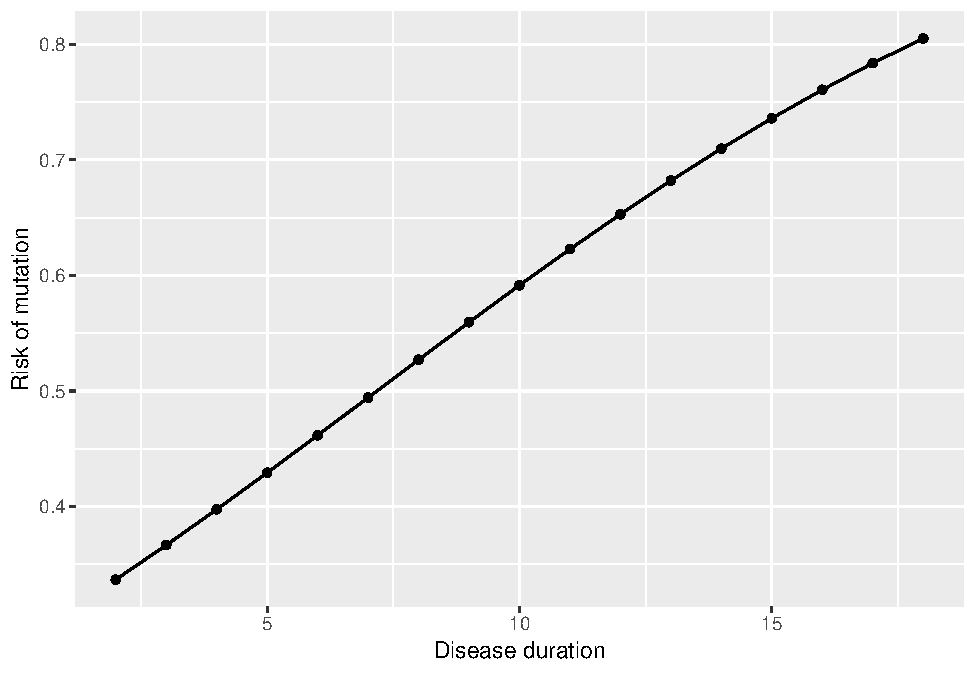
\includegraphics{09-answers_files/figure-latex/week5l-1.pdf}

You can also use the \texttt{augment} function for linear regression and multivariable models. One other interesting thing you can do is to make ``out of sample'' predictions.

Try this:

\begin{Shaded}
\begin{Highlighting}[]
\CommentTok{# Reopen lesson5b dataset}
\NormalTok{lesson5b <-}\StringTok{ }\KeywordTok{readRDS}\NormalTok{(here}\OperatorTok{::}\KeywordTok{here}\NormalTok{(}\StringTok{"Data"}\NormalTok{, }\StringTok{"Week 5"}\NormalTok{, }\StringTok{"lesson5b.rds"}\NormalTok{))}

\CommentTok{# Use original logistic regression model}
\KeywordTok{tbl_regression}\NormalTok{(mutate_model, }\DataTypeTok{exponentiate =} \OtherTok{TRUE}\NormalTok{)}
\end{Highlighting}
\end{Shaded}

\captionsetup[table]{labelformat=empty,skip=1pt}
\begin{longtable}{lccc}
\toprule
\textbf{N = 124} & \textbf{OR}\textsuperscript{1} & \textbf{95\% CI}\textsuperscript{1} & \textbf{p-value} \\ 
\midrule
c & 1.14 & 1.03, 1.27 & 0.014 \\ 
\bottomrule
\end{longtable}
\vspace{-5mm}
\begin{minipage}{\linewidth}
\textsuperscript{1}OR = Odds Ratio, CI = Confidence Interval \\ 
\end{minipage}

\begin{Shaded}
\begin{Highlighting}[]
\CommentTok{# Create new values for "c" (disease duration)}
\NormalTok{lesson5b_new <-}
\StringTok{  }\NormalTok{lesson5b }\OperatorTok
\StringTok{  }\KeywordTok{mutate}\NormalTok{(}\DataTypeTok{c =} \DecValTok{1}\OperatorTok{:}\KeywordTok{n}\NormalTok{()}\OperatorTok{/}\DecValTok{3}\NormalTok{)}
\CommentTok{# "1:n()" gives the observation number for each observation}
\CommentTok{# Replace c with observation number / 3 gives a list of simulated}
\CommentTok{# disease durations between 0.33 and 42.33.}

\CommentTok{# Predict risk of mutation}
\NormalTok{lesson5b_pred <-}
\StringTok{  }\KeywordTok{augment}\NormalTok{(mutate_model,}
          \DataTypeTok{newdata =}\NormalTok{ lesson5b_new,}
          \DataTypeTok{type.predict =} \StringTok{"response"}\NormalTok{)}

\CommentTok{# Create graph}
\KeywordTok{ggplot}\NormalTok{(}\DataTypeTok{data =}\NormalTok{ lesson5b_pred,}
       \KeywordTok{aes}\NormalTok{(}\DataTypeTok{x =}\NormalTok{ c, }\DataTypeTok{y =}\NormalTok{ .fitted)) }\OperatorTok{+}
\StringTok{  }\KeywordTok{geom_line}\NormalTok{()}
\end{Highlighting}
\end{Shaded}

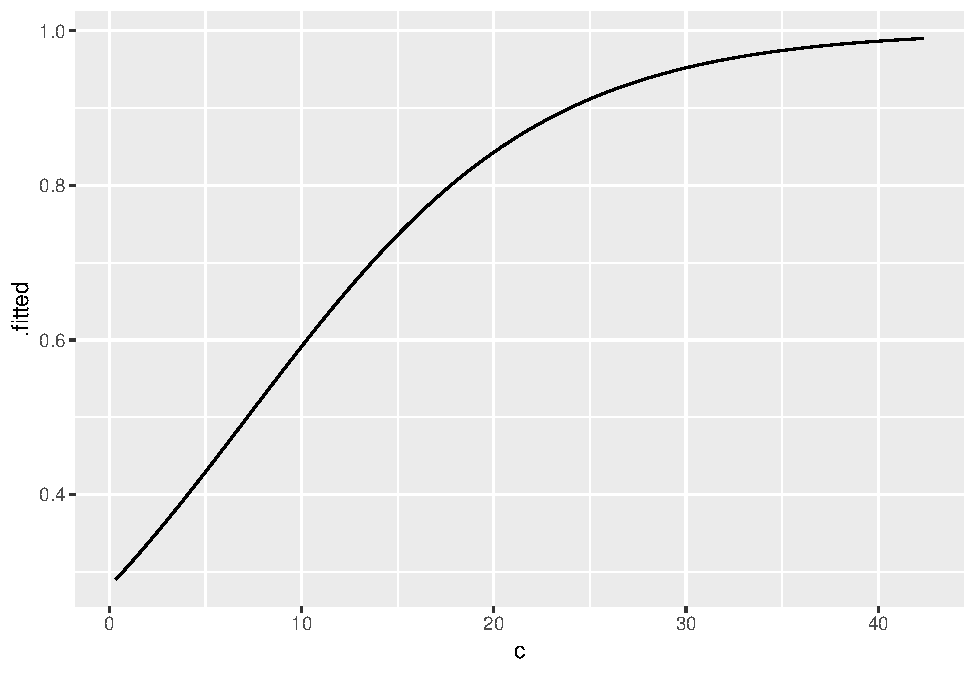
\includegraphics{09-answers_files/figure-latex/week5n-1.pdf}

\hypertarget{lesson5c.rds}{%
\subsection{lesson5c.rds}\label{lesson5c.rds}}

\textbf{These are data from Canadian provinces giving population, unemployment rates and male and female life expectancy. Which of these variables are associated?}

A key first question: what are we likely to be interested in? For example, total population and unemployment rate will have no illuminating relationship whatsoever and we wouldn't want to analyze the association between these two. The link between unemployment and life expectancy seems more interesting. Before we start doing the analysis however, we need to look at the data.

\begin{Shaded}
\begin{Highlighting}[]
\CommentTok{# Open up dataset to view observations}
\KeywordTok{View}\NormalTok{(lesson5c)}
\end{Highlighting}
\end{Shaded}

It seems that there are not only data for each province separately but for Canada as a whole. Clearly we would have to delete this row as it is not an independent observation.

\begin{Shaded}
\begin{Highlighting}[]
\NormalTok{lesson5c_fixed <-}
\StringTok{  }\NormalTok{lesson5c }\OperatorTok
\StringTok{  }\KeywordTok{filter}\NormalTok{(place }\OperatorTok{!=}\StringTok{ "Canada"}\NormalTok{)}
\end{Highlighting}
\end{Shaded}

Now, we could just correlate the three variables together:

\begin{Shaded}
\begin{Highlighting}[]
\CommentTok{# There are missing values for unemployment, so we need to indicate that we only want to use "complete observations"}
\KeywordTok{cor}\NormalTok{(lesson5c_fixed }\OperatorTok\StringTok{ }\KeywordTok{select}\NormalTok{(unemp, mlife, flife),}
    \DataTypeTok{use =} \StringTok{"complete.obs"}\NormalTok{)}
\end{Highlighting}
\end{Shaded}

\begin{verbatim}
##            unemp      mlife      flife
## unemp  1.0000000 -0.7413079 -0.6152419
## mlife -0.7413079  1.0000000  0.7619491
## flife -0.6152419  0.7619491  1.0000000
\end{verbatim}

This tells you that unemployment rates are negatively correlated with life expectancy (i.e.~the higher the unemployment rate, the lower the life expectancy), that this effect seems stronger for men than for women and that male and female life expectancy are strongly correlated.

We might also want to go on and do some regressions. We probably wouldn't ever want to predict the unemployment rate on the basis of life expectancy, but the opposite case is indeed of interest: we might want to know, for example, what effect a 1\% drop in unemployment rate might have on life expectancy.

Try these regression models:

\begin{Shaded}
\begin{Highlighting}[]
\NormalTok{mlife_model <-}\StringTok{ }\KeywordTok{lm}\NormalTok{(mlife }\OperatorTok{~}\StringTok{ }\NormalTok{unemp, }\DataTypeTok{data =}\NormalTok{ lesson5c_fixed)}
\KeywordTok{tbl_regression}\NormalTok{(mlife_model)}
\end{Highlighting}
\end{Shaded}

\captionsetup[table]{labelformat=empty,skip=1pt}
\begin{longtable}{lccc}
\toprule
\textbf{N = 10} & \textbf{Coefficient} & \textbf{95\% CI}\textsuperscript{1} & \textbf{p-value} \\ 
\midrule
\% 15+ population unemployed, 1995 & -0.10 & -0.18, -0.03 & 0.014 \\ 
\bottomrule
\end{longtable}
\vspace{-5mm}
\begin{minipage}{\linewidth}
\textsuperscript{1}CI = Confidence Interval \\ 
\end{minipage}

\begin{Shaded}
\begin{Highlighting}[]
\NormalTok{flife_model <-}\StringTok{ }\KeywordTok{lm}\NormalTok{(flife }\OperatorTok{~}\StringTok{ }\NormalTok{unemp, }\DataTypeTok{data =}\NormalTok{ lesson5c_fixed)}
\KeywordTok{tbl_regression}\NormalTok{(flife_model)}
\end{Highlighting}
\end{Shaded}

\captionsetup[table]{labelformat=empty,skip=1pt}
\begin{longtable}{lccc}
\toprule
\textbf{N = 10} & \textbf{Coefficient} & \textbf{95\% CI}\textsuperscript{1} & \textbf{p-value} \\ 
\midrule
\% 15+ population unemployed, 1995 & -0.08 & -0.17, 0.00 & 0.058 \\ 
\bottomrule
\end{longtable}
\vspace{-5mm}
\begin{minipage}{\linewidth}
\textsuperscript{1}CI = Confidence Interval \\ 
\end{minipage}

The coefficients you get (-0.10 for men and -0.08 for women) suggest that a 5\% drop in unemployment is associated with about a 6 month increase in life expectancy, in other words, a small effect.

Interesting question: should you also report a p value and 95\% confidence interval for the coefficients? The answer is no. This is because Canadian provinces are not some random sample from a large theoretical population of Canadian provinces. You have all the data. So questions of inference (i.e.~p values) and uncertainty (i.e.~95\% confidence intervals) don't come into it.

Even more interesting question: the conclusion of a 5\% drop in unemployment being associated with a 6 month increase in life expectancy is based on a causal relationship, that is, we believe that changes in unemployment \emph{cause} changes in life expectancy. This is not implausible: unemployment leads to poverty and depression, both of which reduce life expectancy. However, a causal relationship cannot be assumed. For example, it may be that life expectancy is lower in certain areas of the country (due to eating patterns or ethnic differences) that also happen to suffer higher unemployment.

\hypertarget{lesson5d.rds}{%
\subsection{lesson5d.rds}\label{lesson5d.rds}}

\textbf{These are data from mice inoculated with tumor cells and then treated with different doses of a drug. The growth rate of each animal's tumor is then calculated. Is this drug effective?}

This is a straightforward linear regression that shows a significant decrease in log tumor size with increasing dose.

\begin{Shaded}
\begin{Highlighting}[]
\NormalTok{tumorsize_model <-}\StringTok{ }\KeywordTok{lm}\NormalTok{(s }\OperatorTok{~}\StringTok{ }\NormalTok{dose, }\DataTypeTok{data =}\NormalTok{ lesson5d)}
\KeywordTok{summary}\NormalTok{(tumorsize_model)}
\end{Highlighting}
\end{Shaded}

\begin{verbatim}
## 
## Call:
## lm(formula = s ~ dose, data = lesson5d)
## 
## Residuals:
##       Min        1Q    Median        3Q       Max 
## -0.026182 -0.010515 -0.005768  0.009948  0.050698 
## 
## Coefficients:
##               Estimate Std. Error t value Pr(>|t|)    
## (Intercept)  5.272e-02  5.376e-03   9.807 1.19e-07 ***
## dose        -7.986e-05  2.674e-05  -2.986  0.00982 ** 
## ---
## Signif. codes:  0 '***' 0.001 '**' 0.01 '*' 0.05 '.' 0.1 ' ' 1
## 
## Residual standard error: 0.01793 on 14 degrees of freedom
## Multiple R-squared:  0.3891, Adjusted R-squared:  0.3454 
## F-statistic: 8.916 on 1 and 14 DF,  p-value: 0.00982
\end{verbatim}

A couple of thoughts. Firstly, this rather obvious analysis is not often conducted in lab research. Typically, researchers present pairwise comparisons between each dose and control. For example, see the following typical diagram. Each of the p values compares the dose to control. The problem with such an approach is that you end up with multiple p values (instead of just one) and that each test takes place in a vacuum: the p value of a comparison between no treatment and, say, dose level 3, is the same regardless of whether there were 2 dose levels in the experiment, or 100, and whether all other dose levels showed an effect or did not. A regression analysis gives you a single p value and uses all data in one analysis.

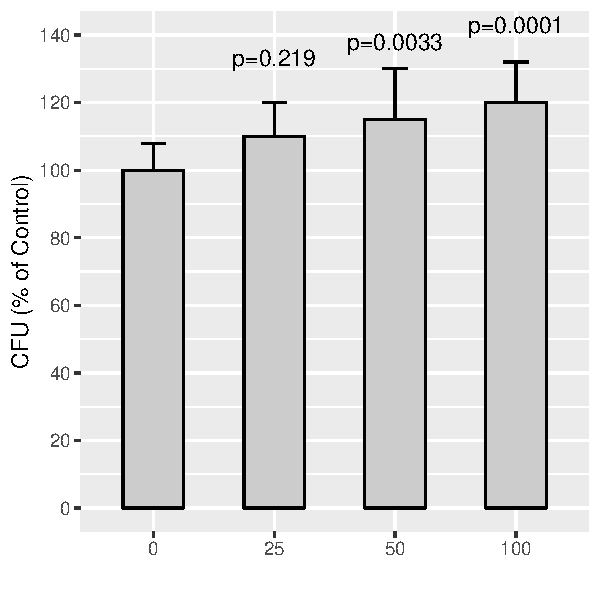
\includegraphics{09-answers_files/figure-latex/week5u-1.pdf}

A second thought: should you report the coefficient of -0.00008? This can be interpreted as ``for each increase in dose of one unit, increase in log tumor size is less by -0.00008''. I would argue that this coefficient might misleading because you only have a few doses and they are widely spaced. Also, dose-response is often non-linear: it generally takes a sigmoidal curve (see below). In short, you might have too few data to be confident about a linear prediction. Finally, it is rare that you really want to estimate the effects of a treatment on a mouse: generally, laboratory studies are about testing hypotheses.

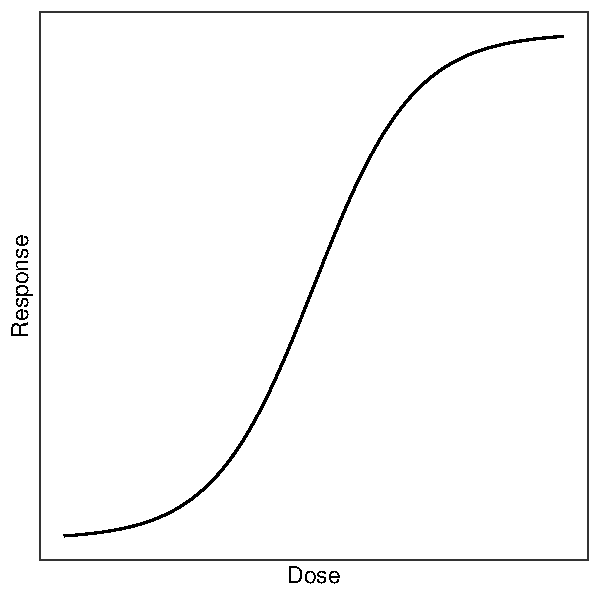
\includegraphics{09-answers_files/figure-latex/week5v-1.pdf}

My model answer would be:

\begin{quote}
Mean increase in log tumor size per day by dose is given in the table. Higher doses were associated with lower growth rates (p=0.010 by linear regression).
\end{quote}

\captionsetup[table]{labelformat=empty,skip=1pt}
\begin{longtable}{rl}
\toprule
Dose & Mean (SD) \\ 
\midrule
0 & 0.069 (0.025) \\ 
4 & 0.046 (0.016) \\ 
40 & 0.039 (0.001) \\ 
400 & 0.022 (0.009) \\ 
\bottomrule
\end{longtable}

\hypertarget{lesson5e.rds}{%
\subsection{lesson5e.rds}\label{lesson5e.rds}}

\textbf{These are data from a study of the use of complementary medicine (e.g.~massage) by UK breast cancer patients. There are data for the women's age, time since diagnosis, presence of distant metastases, use of complementary medicine before diagnosis, whether they received a qualification after high school, the age they left education, whether usual employment is a manual trade, socioeconomic status. What predicts use of complementary medicine by women with breast cancer?}

This is a fairly simple analysis: the outcome is binary and as we want to make predictions we are going to want a logistic regression. It would be tempting just to throw all the variables into the analysis:

\begin{Shaded}
\begin{Highlighting}[]
\NormalTok{cam_model1 <-}\StringTok{ }\KeywordTok{glm}\NormalTok{(CAM }\OperatorTok{~}\StringTok{ }\NormalTok{age }\OperatorTok{+}\StringTok{ }\NormalTok{t }\OperatorTok{+}\StringTok{ }\NormalTok{mets }\OperatorTok{+}\StringTok{ }\NormalTok{u }\OperatorTok{+}\StringTok{ }\NormalTok{q18 }\OperatorTok{+}\StringTok{ }\NormalTok{e }\OperatorTok{+}\StringTok{ }\NormalTok{m }\OperatorTok{+}\StringTok{ }\NormalTok{ses,}
                  \DataTypeTok{data =}\NormalTok{ lesson5e,}
                  \DataTypeTok{family =} \StringTok{"binomial"}\NormalTok{)}
\KeywordTok{tbl_regression}\NormalTok{(cam_model1, }\DataTypeTok{exponentiate =} \OtherTok{TRUE}\NormalTok{)}
\end{Highlighting}
\end{Shaded}

\captionsetup[table]{labelformat=empty,skip=1pt}
\begin{longtable}{lccc}
\toprule
\textbf{N = 438} & \textbf{OR}\textsuperscript{1} & \textbf{95\% CI}\textsuperscript{1} & \textbf{p-value} \\ 
\midrule
age & 0.97 & 0.95, 0.99 & 0.004 \\ 
time since diagnosis & 1.02 & 0.91, 1.15 & 0.7 \\ 
distant metastases? & 1.45 & 0.12, 15.3 & 0.8 \\ 
used CAM before diagnosis? & 7.40 & 4.23, 13.5 & <0.001 \\ 
qualifications after 18? & 2.07 & 1.16, 3.73 & 0.015 \\ 
age left education & 0.93 & 0.83, 1.02 & 0.2 \\ 
manual trade? & 1.19 & 0.39, 3.61 & 0.8 \\ 
socioeconomic status 1 - 5 & 0.81 & 0.54, 1.22 & 0.3 \\ 
\bottomrule
\end{longtable}
\vspace{-5mm}
\begin{minipage}{\linewidth}
\textsuperscript{1}OR = Odds Ratio, CI = Confidence Interval \\ 
\end{minipage}

This would suggest that the strongest predictor is whether women used complementary medicine before diagnosis and that two other variables are predictive: women with a qualification after leaving high school are more likely to use complementary medicine, but use declines with age (older people are more conservative, or alternatively, wiser, depending on your point of view.)

However\ldots{}

Should we just throw everything in the model? For example, only 6 patients have distant metastases. Secondly, many of the variables seem highly correlated. For example, age at which the patient left education and whether they received a qualification after the age of 18 are highly correlated as are socioeconomic status and whether the patient's job is a manual trade. In clinical terms, you wouldn't need to know the age that someone left education if you already knew whether they had a post-high school qualification. And as would be intuitive, regression does not deal well with correlated variables. To take an extreme example, take two variables ``x'' which is equal to height, and ``y'' which is equal to height plus 1 inch. These have a correlation of one. Regressing just variable x or y on shoe size you get:

\(shoesize = 0.6*x - 30\)

or

\(shoesize = 0.6*y - 31\)

What would you get for regressing x and y? Any of the following are possible:

\(shoesize = 0.3*x + 0.3*y - 30.5\)

\(shoesize = 0.4*x + 0.2*y - 30.5\)

\(shoesize = 0.1*x + 0.5*y - 30.5\)

There is no way of telling these apart in terms of regression. Bottom line: care is needed with correlated variables both in a clinical / scientific sense (you don't need both of two correlated variables in a model) and a statistical sense (regression results can be misleading).

So I would start with the full model and then remove the least predictive of socioeconomic status and manual trade, and the least predictive of qualification and age left education. You end up with:

\begin{Shaded}
\begin{Highlighting}[]
\NormalTok{cam_model2 <-}\StringTok{ }\KeywordTok{glm}\NormalTok{(CAM }\OperatorTok{~}\StringTok{ }\NormalTok{age }\OperatorTok{+}\StringTok{ }\NormalTok{t }\OperatorTok{+}\StringTok{ }\NormalTok{mets }\OperatorTok{+}\StringTok{ }\NormalTok{u }\OperatorTok{+}\StringTok{ }\NormalTok{q18 }\OperatorTok{+}\StringTok{ }\NormalTok{ses,}
                  \DataTypeTok{data =}\NormalTok{ lesson5e,}
                  \DataTypeTok{family =} \StringTok{"binomial"}\NormalTok{)}
\KeywordTok{tbl_regression}\NormalTok{(cam_model2, }\DataTypeTok{exponentiate =} \OtherTok{TRUE}\NormalTok{)}
\end{Highlighting}
\end{Shaded}

\captionsetup[table]{labelformat=empty,skip=1pt}
\begin{longtable}{lccc}
\toprule
\textbf{N = 445} & \textbf{OR}\textsuperscript{1} & \textbf{95\% CI}\textsuperscript{1} & \textbf{p-value} \\ 
\midrule
age & 0.97 & 0.95, 0.99 & 0.004 \\ 
time since diagnosis & 1.02 & 0.91, 1.15 & 0.7 \\ 
distant metastases? & 1.36 & 0.11, 14.8 & 0.8 \\ 
used CAM before diagnosis? & 7.21 & 4.16, 12.9 & <0.001 \\ 
qualifications after 18? & 1.71 & 1.04, 2.80 & 0.033 \\ 
socioeconomic status 1 - 5 & 0.88 & 0.73, 1.07 & 0.2 \\ 
\bottomrule
\end{longtable}
\vspace{-5mm}
\begin{minipage}{\linewidth}
\textsuperscript{1}OR = Odds Ratio, CI = Confidence Interval \\ 
\end{minipage}

Now it appears that ``q18'' is predictive but not ``ses''. So try removing one of these from the model in turn:

\begin{Shaded}
\begin{Highlighting}[]
\NormalTok{cam_model3 <-}\StringTok{ }\KeywordTok{glm}\NormalTok{(CAM }\OperatorTok{~}\StringTok{ }\NormalTok{age }\OperatorTok{+}\StringTok{ }\NormalTok{t }\OperatorTok{+}\StringTok{ }\NormalTok{mets }\OperatorTok{+}\StringTok{ }\NormalTok{u }\OperatorTok{+}\StringTok{ }\NormalTok{ses,}
                  \DataTypeTok{data =}\NormalTok{ lesson5e,}
                  \DataTypeTok{family =} \StringTok{"binomial"}\NormalTok{)}
\KeywordTok{tbl_regression}\NormalTok{(cam_model3, }\DataTypeTok{exponentiate =} \OtherTok{TRUE}\NormalTok{)}
\end{Highlighting}
\end{Shaded}

\captionsetup[table]{labelformat=empty,skip=1pt}
\begin{longtable}{lccc}
\toprule
\textbf{N = 459} & \textbf{OR}\textsuperscript{1} & \textbf{95\% CI}\textsuperscript{1} & \textbf{p-value} \\ 
\midrule
age & 0.97 & 0.95, 0.99 & 0.002 \\ 
time since diagnosis & 1.04 & 0.93, 1.17 & 0.5 \\ 
distant metastases? & 1.23 & 0.10, 13.4 & 0.9 \\ 
used CAM before diagnosis? & 7.65 & 4.45, 13.6 & <0.001 \\ 
socioeconomic status 1 - 5 & 0.78 & 0.66, 0.93 & 0.005 \\ 
\bottomrule
\end{longtable}
\vspace{-5mm}
\begin{minipage}{\linewidth}
\textsuperscript{1}OR = Odds Ratio, CI = Confidence Interval \\ 
\end{minipage}

\begin{Shaded}
\begin{Highlighting}[]
\NormalTok{cam_model4 <-}\StringTok{ }\KeywordTok{glm}\NormalTok{(CAM }\OperatorTok{~}\StringTok{ }\NormalTok{age }\OperatorTok{+}\StringTok{ }\NormalTok{t }\OperatorTok{+}\StringTok{ }\NormalTok{mets }\OperatorTok{+}\StringTok{ }\NormalTok{u }\OperatorTok{+}\StringTok{ }\NormalTok{q18,}
                  \DataTypeTok{data =}\NormalTok{ lesson5e,}
                  \DataTypeTok{family =} \StringTok{"binomial"}\NormalTok{)}
\KeywordTok{tbl_regression}\NormalTok{(cam_model4, }\DataTypeTok{exponentiate =} \OtherTok{TRUE}\NormalTok{)}
\end{Highlighting}
\end{Shaded}

\captionsetup[table]{labelformat=empty,skip=1pt}
\begin{longtable}{lccc}
\toprule
\textbf{N = 651} & \textbf{OR}\textsuperscript{1} & \textbf{95\% CI}\textsuperscript{1} & \textbf{p-value} \\ 
\midrule
age & 0.96 & 0.94, 0.97 & <0.001 \\ 
time since diagnosis & 1.01 & 0.92, 1.12 & 0.8 \\ 
distant metastases? & 0.85 & 0.08, 6.83 & 0.9 \\ 
used CAM before diagnosis? & 7.32 & 4.48, 12.3 & <0.001 \\ 
qualifications after 18? & 1.90 & 1.28, 2.82 & 0.002 \\ 
\bottomrule
\end{longtable}
\vspace{-5mm}
\begin{minipage}{\linewidth}
\textsuperscript{1}OR = Odds Ratio, CI = Confidence Interval \\ 
\end{minipage}

It turns out that both are predictive independently, but not together. When you think about this, it is because socioeconomic status is correlated with education. The most sensible thing to do is to leave ``q18'' in the model as a) it is slightly more predictive and b) it is easier to ask about; c) there are fewer missing data. As such, my model answer might be:

\begin{quote}
There were responses from 714 women, of whom had data adequate for analysis. There were more missing data for socioeconomic status but this was not included in the final model. In a multivariable model, use of complementary medicine before diagnosis was the strongest predictor of complementary medicine use in women with breast cancer, odds ratio 7.32 (95\% CI 4.48, 12.3; p\textless0.001). Complementary medicine use was related to education. The odds of a woman with a qualification received after the age of 18 using complementary medicine were 1.90 (95\% CI 1.28, 2.82; p=0.002) those of women without a qualification after high school. In a univariate model, higher socioeconomic status predicted use of complementary medicine, but this was dropped from the multivariable model due to collinearity with educational achievement. Older women were less likely to use complementary medicine (odds ratio 0.96 for a one-year increase in age; 95\% CI 0.94, 0.97, p\textless0.001). There was no statistically significant effect of time since diagnosis (odds ratio 1.01 per year; 95\% CI 0.92, 1.12, p=0.8). This suggests that breast cancer patients who use complementary medicine are likely to start doing so shortly after diagnosis.
\end{quote}

\hypertarget{lesson5f.rds}{%
\subsection{lesson5f.rds}\label{lesson5f.rds}}

\textbf{These are the distance records for Frisbee for various ages in males. What is the relationship between age and how far a man can throw a Frisbee?}

Well the obvious thing to do would be a linear regression:

\begin{Shaded}
\begin{Highlighting}[]
\NormalTok{frisbee_model <-}\StringTok{ }\KeywordTok{lm}\NormalTok{(distance }\OperatorTok{~}\StringTok{ }\NormalTok{age,}
                    \DataTypeTok{data =}\NormalTok{ lesson5f)}
\KeywordTok{summary}\NormalTok{(frisbee_model)}
\end{Highlighting}
\end{Shaded}

\begin{verbatim}
## 
## Call:
## lm(formula = distance ~ age, data = lesson5f)
## 
## Residuals:
##     Min      1Q  Median      3Q     Max 
## -90.772 -53.291   4.797  43.120 105.031 
## 
## Coefficients:
##             Estimate Std. Error t value Pr(>|t|)    
## (Intercept)   88.165     20.447   4.312 0.000717 ***
## age            1.623      0.673   2.412 0.030187 *  
## ---
## Signif. codes:  0 '***' 0.001 '**' 0.01 '*' 0.05 '.' 0.1 ' ' 1
## 
## Residual standard error: 56.94 on 14 degrees of freedom
## Multiple R-squared:  0.2935, Adjusted R-squared:  0.243 
## F-statistic: 5.816 on 1 and 14 DF,  p-value: 0.03019
\end{verbatim}

You get a coefficient of 1.62, meaning that the furthest a man can throw a Frisbee increases by 1.62 meters every year. But of course this is nonsense: you can't throw further and further each year, athletic ability starts to decline with age. You can see this on a graph:

\begin{Shaded}
\begin{Highlighting}[]
\KeywordTok{ggplot}\NormalTok{(}\DataTypeTok{data =}\NormalTok{ lesson5f,}
       \KeywordTok{aes}\NormalTok{(}\DataTypeTok{x =}\NormalTok{ age, }\DataTypeTok{y =}\NormalTok{ distance)) }\OperatorTok{+}\StringTok{ }
\StringTok{  }\KeywordTok{geom_point}\NormalTok{()}
\end{Highlighting}
\end{Shaded}

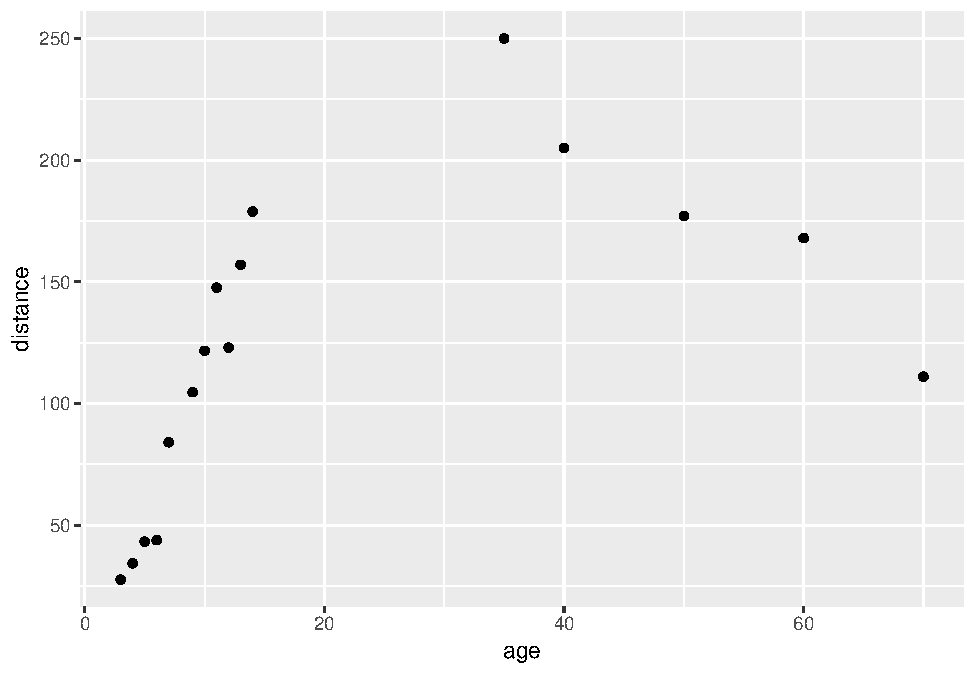
\includegraphics{09-answers_files/figure-latex/week53-1.pdf}

In other words, there is not a linear relationship between your age and the distance you can throw a Frisbee. There are two options. You can either do two linear regressions, one for age up to 30 and one for age \textgreater30. But this is a little sloppy: better, you could try including non-linear terms (see below). In either case, remember not to report p values or 95\% confidence intervals: these are meaningless because there is only one record per distance.

\emph{For advanced students only:}

Often the relationship between an \(x\) and a \(y\) does not follow a straight line. You may remember from high school that one way to get a curve is to have a quadratic equation including both \(x\) and \(x^2\). So you have to create a new variable called age2 as ``age2 = age\^{}2'' and regress:

\begin{Shaded}
\begin{Highlighting}[]
\NormalTok{lesson5f <-}
\StringTok{  }\NormalTok{lesson5f }\OperatorTok
\StringTok{  }\KeywordTok{mutate}\NormalTok{(}
    \DataTypeTok{age2 =}\NormalTok{ age}\OperatorTok{^}\DecValTok{2}
\NormalTok{  )}

\NormalTok{frisbee_model2 <-}\StringTok{ }\KeywordTok{lm}\NormalTok{(distance }\OperatorTok{~}\StringTok{ }\NormalTok{age }\OperatorTok{+}\StringTok{ }\NormalTok{age2,}
                     \DataTypeTok{data =}\NormalTok{ lesson5f)}
\KeywordTok{summary}\NormalTok{(frisbee_model2)}
\end{Highlighting}
\end{Shaded}

\begin{verbatim}
## 
## Call:
## lm(formula = distance ~ age + age2, data = lesson5f)
## 
## Residuals:
##     Min      1Q  Median      3Q     Max 
## -38.530 -18.159   1.256  19.124  37.573 
## 
## Coefficients:
##             Estimate Std. Error t value Pr(>|t|)    
## (Intercept)  8.13134   13.41881   0.606    0.555    
## age         11.60072    1.29513   8.957 6.36e-07 ***
## age2        -0.14906    0.01886  -7.905 2.55e-06 ***
## ---
## Signif. codes:  0 '***' 0.001 '**' 0.01 '*' 0.05 '.' 0.1 ' ' 1
## 
## Residual standard error: 24.52 on 13 degrees of freedom
## Multiple R-squared:  0.8783, Adjusted R-squared:  0.8596 
## F-statistic: 46.92 on 2 and 13 DF,  p-value: 1.132e-06
\end{verbatim}

This model (distance = 11.6\emph{age - 0.149}age\^{}2 + 8.13) fits extremely well (r\textsuperscript{2} of 0.88 vs 0.29 for the linear model). If you really remember your high school match, consider that for a regression equation \(y = ax + bx^2 + c\) you can work out the maximum \(y\) as \(-a/2b\). We predict that the world record for distance will be held by a man who is -11.6/(2 * -0.149) = 38.9 years old.

\hypertarget{lesson5g.rds}{%
\subsection{lesson5g.rds}\label{lesson5g.rds}}

\textbf{You've seen this data set before. Patients with lung cancer are randomized to receive either chemotherapy regime a or b and assessed for tumor response. We know there is no difference between regimes (you can test this if you like). However, do the treatments work differently depending on age or sex?}

The first thing to do here is to do the sub-group analysis, just to get a feel for the data.

Try this:

\begin{Shaded}
\begin{Highlighting}[]
\CommentTok{# For men}
\KeywordTok{tbl_summary}\NormalTok{(}
\NormalTok{  lesson5g }\OperatorTok\StringTok{ }\KeywordTok{filter}\NormalTok{(sex }\OperatorTok{==}\StringTok{ }\DecValTok{0}\NormalTok{) }\OperatorTok\StringTok{ }\KeywordTok{select}\NormalTok{(response, chemo),}
  \DataTypeTok{by =} \StringTok{"chemo"}\NormalTok{,}
  \DataTypeTok{type =} \KeywordTok{list}\NormalTok{(}\DataTypeTok{response =} \StringTok{"categorical"}\NormalTok{)}
\NormalTok{)}
\end{Highlighting}
\end{Shaded}

\captionsetup[table]{labelformat=empty,skip=1pt}
\begin{longtable}{lcc}
\toprule
\textbf{Characteristic}\textsuperscript{1} & \textbf{0}, N = 138 & \textbf{1}, N = 156 \\ 
\midrule
1 = response to treatment, 0 = failure &  &  \\ 
0 & 84 (61\%) & 76 (49\%) \\ 
1 & 54 (39\%) & 80 (51\%) \\ 
\bottomrule
\end{longtable}
\vspace{-5mm}
\begin{minipage}{\linewidth}
\textsuperscript{1}Statistics presented: n (\%) \\ 
\end{minipage}

\begin{Shaded}
\begin{Highlighting}[]
\CommentTok{# For women}
\KeywordTok{tbl_summary}\NormalTok{(}
\NormalTok{  lesson5g }\OperatorTok\StringTok{ }\KeywordTok{filter}\NormalTok{(sex }\OperatorTok{==}\StringTok{ }\DecValTok{1}\NormalTok{) }\OperatorTok\StringTok{ }\KeywordTok{select}\NormalTok{(response, chemo),}
  \DataTypeTok{by =} \StringTok{"chemo"}\NormalTok{,}
  \DataTypeTok{type =} \KeywordTok{list}\NormalTok{(}\DataTypeTok{response =} \StringTok{"categorical"}\NormalTok{)}
\NormalTok{)}
\end{Highlighting}
\end{Shaded}

\captionsetup[table]{labelformat=empty,skip=1pt}
\begin{longtable}{lcc}
\toprule
\textbf{Characteristic}\textsuperscript{1} & \textbf{0}, N = 62 & \textbf{1}, N = 44 \\ 
\midrule
1 = response to treatment, 0 = failure &  &  \\ 
0 & 35 (56\%) & 27 (61\%) \\ 
1 & 27 (44\%) & 17 (39\%) \\ 
\bottomrule
\end{longtable}
\vspace{-5mm}
\begin{minipage}{\linewidth}
\textsuperscript{1}Statistics presented: n (\%) \\ 
\end{minipage}

\begin{Shaded}
\begin{Highlighting}[]
\CommentTok{# Here, summarize stores out the p values for the chi-squared test by sex}
\NormalTok{lesson5g }\OperatorTok
\StringTok{  }\KeywordTok{group_by}\NormalTok{(sex) }\OperatorTok
\StringTok{  }\KeywordTok{summarize}\NormalTok{(}\DataTypeTok{p =} \KeywordTok{chisq.test}\NormalTok{(response, chemo, }\DataTypeTok{correct =} \OtherTok{FALSE}\NormalTok{)}\OperatorTok{$}\NormalTok{p.value)}
\end{Highlighting}
\end{Shaded}

\begin{verbatim}
## # A tibble: 2 x 2
##     sex      p
##   <dbl>  <dbl>
## 1     0 0.0368
## 2     1 0.613
\end{verbatim}

This shows that regime b is better for men (51\% vs 39\% response rate, p=0.037). For women, there doesn't seem to be a difference between groups. The next thing to check is whether sex in general makes a difference to response:

\begin{Shaded}
\begin{Highlighting}[]
\KeywordTok{tbl_summary}\NormalTok{(}
\NormalTok{  lesson5g }\OperatorTok\StringTok{ }\KeywordTok{select}\NormalTok{(response, sex),}
  \DataTypeTok{by =} \StringTok{"sex"}\NormalTok{,}
  \DataTypeTok{type =} \KeywordTok{list}\NormalTok{(}\DataTypeTok{response =} \StringTok{"categorical"}\NormalTok{)}
\NormalTok{)}
\end{Highlighting}
\end{Shaded}

\captionsetup[table]{labelformat=empty,skip=1pt}
\begin{longtable}{lcc}
\toprule
\textbf{Characteristic}\textsuperscript{1} & \textbf{0}, N = 294 & \textbf{1}, N = 106 \\ 
\midrule
1 = response to treatment, 0 = failure &  &  \\ 
0 & 160 (54\%) & 62 (58\%) \\ 
1 & 134 (46\%) & 44 (42\%) \\ 
\bottomrule
\end{longtable}
\vspace{-5mm}
\begin{minipage}{\linewidth}
\textsuperscript{1}Statistics presented: n (\%) \\ 
\end{minipage}

\begin{Shaded}
\begin{Highlighting}[]
\KeywordTok{table}\NormalTok{(lesson5g}\OperatorTok{$}\NormalTok{response, lesson5g}\OperatorTok{$}\NormalTok{sex) }\OperatorTok
\StringTok{  }\KeywordTok{chisq.test}\NormalTok{(}\DataTypeTok{correct =} \OtherTok{FALSE}\NormalTok{)}
\end{Highlighting}
\end{Shaded}

\begin{verbatim}
## 
##  Pearson's Chi-squared test
## 
## data:  .
## X-squared = 0.52224, df = 1, p-value = 0.4699
\end{verbatim}

This shows similar response rates (around 40-45\%) for men and women.

Now we want to test for interaction between chemo regime and sex in a multivariable regression. You can put the interaction directly into the multivariable model:

\begin{Shaded}
\begin{Highlighting}[]
\NormalTok{sex_int_model <-}\StringTok{ }\KeywordTok{glm}\NormalTok{(response }\OperatorTok{~}\StringTok{ }\NormalTok{sex }\OperatorTok{+}\StringTok{ }\NormalTok{chemo }\OperatorTok{+}\StringTok{ }\NormalTok{sex}\OperatorTok{*}\NormalTok{chemo,}
                     \DataTypeTok{data =}\NormalTok{ lesson5g,}
                     \DataTypeTok{family =} \StringTok{"binomial"}\NormalTok{)}
\KeywordTok{tbl_regression}\NormalTok{(sex_int_model, }\DataTypeTok{exponentiate =} \OtherTok{TRUE}\NormalTok{)}
\end{Highlighting}
\end{Shaded}

\captionsetup[table]{labelformat=empty,skip=1pt}
\begin{longtable}{lccc}
\toprule
\textbf{N = 400} & \textbf{OR}\textsuperscript{1} & \textbf{95\% CI}\textsuperscript{1} & \textbf{p-value} \\ 
\midrule
1 if female & 1.20 & 0.65, 2.20 & 0.6 \\ 
0 for regime a, 1 for regime b & 1.64 & 1.03, 2.61 & 0.037 \\ 
1 if female * 0 for regime a, 1 for regime b & 0.50 & 0.20, 1.24 & 0.14 \\ 
\bottomrule
\end{longtable}
\vspace{-5mm}
\begin{minipage}{\linewidth}
\textsuperscript{1}OR = Odds Ratio, CI = Confidence Interval \\ 
\end{minipage}

By the way, don't try \texttt{glm(response\ \textasciitilde{}\ sex*chemo,\ ...)}, that is, including only the interaction term. This would involve a non-randomized comparison between men and women who received the same chemotherapy treatment.

You can repeat this for age by creating a new variable based on the median age:

\begin{Shaded}
\begin{Highlighting}[]
\CommentTok{# First, get the median age}
\KeywordTok{skim}\NormalTok{(lesson5g}\OperatorTok{$}\NormalTok{age)}
\end{Highlighting}
\end{Shaded}

\begin{verbatim}
## 
## Skim summary statistics
## 
## -- Variable type:numeric ---------------------------------------------------------------
##      variable missing complete   n  mean    sd p0   p25  p50 p75 p100
##  lesson5g$age       2      398 400 42.46 10.58 17 34.25 42.5  49   71
##      hist
##  ▁▃▇▇▆▃▂▁
\end{verbatim}

\begin{Shaded}
\begin{Highlighting}[]
\CommentTok{# Then, create a category variable based on median age}
\NormalTok{lesson5g <-}
\StringTok{  }\NormalTok{lesson5g }\OperatorTok
\StringTok{  }\KeywordTok{mutate}\NormalTok{(}
    \DataTypeTok{hiage =} \KeywordTok{if_else}\NormalTok{(age }\OperatorTok{>}\StringTok{ }\FloatTok{42.5}\NormalTok{, }\DecValTok{1}\NormalTok{, }\DecValTok{0}\NormalTok{)}
\NormalTok{  )}
\end{Highlighting}
\end{Shaded}

Then do the subgroup analysis as above:

\begin{Shaded}
\begin{Highlighting}[]
\CommentTok{# For younger patients}
\KeywordTok{tbl_summary}\NormalTok{(}
\NormalTok{  lesson5g }\OperatorTok\StringTok{ }\KeywordTok{filter}\NormalTok{(hiage }\OperatorTok{==}\StringTok{ }\DecValTok{0}\NormalTok{) }\OperatorTok\StringTok{ }\KeywordTok{select}\NormalTok{(response, chemo),}
  \DataTypeTok{by =} \StringTok{"chemo"}\NormalTok{,}
  \DataTypeTok{type =} \KeywordTok{list}\NormalTok{(}\DataTypeTok{response =} \StringTok{"categorical"}\NormalTok{)}
\NormalTok{)}
\end{Highlighting}
\end{Shaded}

\captionsetup[table]{labelformat=empty,skip=1pt}
\begin{longtable}{lcc}
\toprule
\textbf{Characteristic}\textsuperscript{1} & \textbf{0}, N = 96 & \textbf{1}, N = 103 \\ 
\midrule
1 = response to treatment, 0 = failure &  &  \\ 
0 & 52 (54\%) & 47 (46\%) \\ 
1 & 44 (46\%) & 56 (54\%) \\ 
\bottomrule
\end{longtable}
\vspace{-5mm}
\begin{minipage}{\linewidth}
\textsuperscript{1}Statistics presented: n (\%) \\ 
\end{minipage}

\begin{Shaded}
\begin{Highlighting}[]
\CommentTok{# For older patients}
\KeywordTok{tbl_summary}\NormalTok{(}
\NormalTok{  lesson5g }\OperatorTok\StringTok{ }\KeywordTok{filter}\NormalTok{(hiage }\OperatorTok{==}\StringTok{ }\DecValTok{1}\NormalTok{) }\OperatorTok\StringTok{ }\KeywordTok{select}\NormalTok{(response, chemo),}
  \DataTypeTok{by =} \StringTok{"chemo"}\NormalTok{,}
  \DataTypeTok{type =} \KeywordTok{list}\NormalTok{(}\DataTypeTok{response =} \StringTok{"categorical"}\NormalTok{)}
\NormalTok{)}
\end{Highlighting}
\end{Shaded}

\captionsetup[table]{labelformat=empty,skip=1pt}
\begin{longtable}{lcc}
\toprule
\textbf{Characteristic}\textsuperscript{1} & \textbf{0}, N = 102 & \textbf{1}, N = 97 \\ 
\midrule
1 = response to treatment, 0 = failure &  &  \\ 
0 & 66 (65\%) & 56 (58\%) \\ 
1 & 36 (35\%) & 41 (42\%) \\ 
\bottomrule
\end{longtable}
\vspace{-5mm}
\begin{minipage}{\linewidth}
\textsuperscript{1}Statistics presented: n (\%) \\ 
\end{minipage}

\begin{Shaded}
\begin{Highlighting}[]
\NormalTok{lesson5g }\OperatorTok
\StringTok{  }\KeywordTok{filter}\NormalTok{(}\OperatorTok{!}\KeywordTok{is.na}\NormalTok{(age)) }\OperatorTok\StringTok{ }\CommentTok{# Exclude 2 patients missing age}
\StringTok{  }\KeywordTok{group_by}\NormalTok{(hiage) }\OperatorTok
\StringTok{  }\KeywordTok{summarize}\NormalTok{(}\DataTypeTok{p =} \KeywordTok{chisq.test}\NormalTok{(response, chemo, }\DataTypeTok{correct =} \OtherTok{FALSE}\NormalTok{)}\OperatorTok{$}\NormalTok{p.value)}
\end{Highlighting}
\end{Shaded}

\begin{verbatim}
## # A tibble: 2 x 2
##   hiage     p
##   <dbl> <dbl>
## 1     0 0.229
## 2     1 0.313
\end{verbatim}

There do not appear to be any differences between groups. Now to do the interaction analysis, you can create an interaction term in one of two ways (\texttt{chemo*age} or \texttt{chemo*hiage}).

\begin{Shaded}
\begin{Highlighting}[]
\NormalTok{age_int_model1 <-}
\StringTok{  }\KeywordTok{glm}\NormalTok{(response }\OperatorTok{~}\StringTok{ }\NormalTok{chemo }\OperatorTok{+}\StringTok{ }\NormalTok{age }\OperatorTok{+}\StringTok{ }\NormalTok{chemo}\OperatorTok{*}\NormalTok{age,}
      \DataTypeTok{data =}\NormalTok{ lesson5g,}
      \DataTypeTok{family =} \StringTok{"binomial"}\NormalTok{)}
\KeywordTok{tbl_regression}\NormalTok{(age_int_model1, }\DataTypeTok{exponentiate =} \OtherTok{TRUE}\NormalTok{)}
\end{Highlighting}
\end{Shaded}

\captionsetup[table]{labelformat=empty,skip=1pt}
\begin{longtable}{lccc}
\toprule
\textbf{N = 398} & \textbf{OR}\textsuperscript{1} & \textbf{95\% CI}\textsuperscript{1} & \textbf{p-value} \\ 
\midrule
0 for regime a, 1 for regime b & 2.24 & 0.42, 12.1 & 0.3 \\ 
age & 0.98 & 0.96, 1.01 & 0.3 \\ 
0 for regime a, 1 for regime b * age & 0.99 & 0.95, 1.03 & 0.6 \\ 
\bottomrule
\end{longtable}
\vspace{-5mm}
\begin{minipage}{\linewidth}
\textsuperscript{1}OR = Odds Ratio, CI = Confidence Interval \\ 
\end{minipage}

\begin{Shaded}
\begin{Highlighting}[]
\NormalTok{age_int_model2 <-}
\StringTok{  }\KeywordTok{glm}\NormalTok{(response }\OperatorTok{~}\StringTok{ }\NormalTok{chemo }\OperatorTok{+}\StringTok{ }\NormalTok{hiage }\OperatorTok{+}\StringTok{ }\NormalTok{chemo}\OperatorTok{*}\NormalTok{hiage,}
      \DataTypeTok{data =}\NormalTok{ lesson5g,}
      \DataTypeTok{family =} \StringTok{"binomial"}\NormalTok{)}
\KeywordTok{tbl_regression}\NormalTok{(age_int_model2, }\DataTypeTok{exponentiate =} \OtherTok{TRUE}\NormalTok{)}
\end{Highlighting}
\end{Shaded}

\captionsetup[table]{labelformat=empty,skip=1pt}
\begin{longtable}{lccc}
\toprule
\textbf{N = 398} & \textbf{OR}\textsuperscript{1} & \textbf{95\% CI}\textsuperscript{1} & \textbf{p-value} \\ 
\midrule
0 for regime a, 1 for regime b & 1.41 & 0.81, 2.47 & 0.2 \\ 
hiage & 0.64 & 0.36, 1.14 & 0.13 \\ 
0 for regime a, 1 for regime b * hiage & 0.95 & 0.43, 2.12 & >0.9 \\ 
\bottomrule
\end{longtable}
\vspace{-5mm}
\begin{minipage}{\linewidth}
\textsuperscript{1}OR = Odds Ratio, CI = Confidence Interval \\ 
\end{minipage}

Whichever one you choose, the interaction is non-significant in a logistic regression with age and chemotherapy. Incidentally, you must put age in the model because, not surprisingly, it is statistically significant, with higher age being associated with a lower chance of response.

Incidentally, I have often emphasized the importance of including an estimate and a 95\% confidence interval in any set of results rather than just saying ``differences between groups were / were not significant''. Interaction analyses are somewhat of an exception to this general rule. First, these tend to be secondary, exploratory analyses. Secondly, interaction is rather rare in medicine: treatments tend to work (or not work) regardless of a patients age, gender, race and so on. Thirdly, the coefficient for the interaction term can be quite difficult to interpret. So it is often appropriate just to say that you looked for an interaction and didn't find one. A model answer might be:

\begin{quote}
{[}Describe main comparison between chemo regimens here. Describe age and sex here.{]} In a subgroup analysis, there appeared to a differential effect of the two regimens depending on sex. In men, response rates were higher for regimen B (51\%) than regimen A (39\%); response rates were more similar in women, though perhaps favoring regimen A (44\% vs.~39\%). Sex and sex by regimen interaction were entered into a logistic regression model of regimen and response, but the interaction term was non-significant (p=0.14). There were no apparent differences in response depending on age: response rates were 54\% v. 46\% in patients aged below the median compared to 42\% v. 35\% in patients aged above the median. The interaction between regimen and age as a continuous variable was non-significant (p=0.6).
\end{quote}

\hypertarget{lesson5h.rds}{%
\subsection{lesson5h.rds}\label{lesson5h.rds}}

\textbf{PSA is used to screen for prostate cancer. In this data set, the researchers are looking at various forms of PSA (e.g.~``nicked'' PSA). What variables should be used to try to predict prostate cancer? How accurate would this test be?}

One approach to selecting which variables to include in a predictive model would be to do a regression. You could start with all the variables (i.e.~\texttt{glm(cancer\ \textasciitilde{}\ psa\ +\ psan\ +\ psai\ +\ psant,\ ...)}). You might notice that psant is not a good predictor (p=0.3) and decide to take it out of the model. In a regression using the remaining three variables, psai is not statistically significant, and you might then want to remove that variable too. Both psa and psan are highly predictive, so you could leave them in the model and use the \texttt{roc} function (from the \texttt{pROC} package) to get the area-under-the-curve.

However, I would have my doubts about such an approach. What you are trying to do here is predict the presence of cancer as well as you can: the significance or otherwise of individual variables doesn't really come into it. How I would lay about my analysis would be in terms of the area-under-the-curve of the model. So a model answer might be:

\begin{quote}
The cohort consisted of 353 patients. Values for PSA and PSA subtypes are shown in the table. Entering all four PSA variables into a logistic model to predict the presence of prostate cancer gave an area-under-the-curve (AUC) of 0.736. Nicked-to-total ratio was not a strong predictor and removing it from the model did not decrease AUC (0.738). Removing intact PSA from the model had a small but noticeable impact on AUC (0.729). We therefore recommend that further research use total, nicked and intact PSA to predict prostate cancer.
\end{quote}

\textbf{Table 1. Marker distributions}

\captionsetup[table]{labelformat=empty,skip=1pt}
\begin{longtable}{lc}
\toprule
\textbf{Characteristic}\textsuperscript{1} & \textbf{N = 353} \\ 
\midrule
Total PSA (ng/mL) & 6.8 (4.3, 10.2) \\ 
Nicked PSA (ng/mL) & 0.47 (0.28, 0.71) \\ 
Intact PSA (ng/mL) & 0.48 (0.38, 0.57) \\ 
Nicked-to-total ratio & 0.07 (0.05, 0.11) \\ 
\bottomrule
\end{longtable}
\vspace{-5mm}
\begin{minipage}{\linewidth}
\textsuperscript{1}Statistics presented: median (IQR) \\ 
\end{minipage}

*\textbf{Table 2. Multivariable prediction model}

\captionsetup[table]{labelformat=empty,skip=1pt}
\begin{longtable}{lccc}
\toprule
\textbf{N = 353} & \textbf{OR}\textsuperscript{1} & \textbf{95\% CI}\textsuperscript{1} & \textbf{p-value} \\ 
\midrule
Total PSA & 1.30 & 1.20, 1.43 & <0.001 \\ 
Nicked PSA & 0.22 & 0.10, 0.46 & <0.001 \\ 
Intact PSA & 0.41 & 0.13, 1.10 & 0.081 \\ 
\bottomrule
\end{longtable}
\vspace{-5mm}
\begin{minipage}{\linewidth}
\textsuperscript{1}OR = Odds Ratio, CI = Confidence Interval \\ 
\end{minipage}

\hypertarget{lesson5i.rds}{%
\subsection{lesson5i.rds}\label{lesson5i.rds}}

\textbf{This is a randomized trial of behavioral therapy in cancer patients with depressed mood. Patients are randomized to no treatment (group 1), informal contact with a volunteer (group 2) or behavior therapy with a trained therapist (group 3). What would you conclude about the effectiveness of these treatments?}

One approach to these data is to use a test called ANOVA. This addresses the question of whether there is some overall difference between the three groups, or, more specifically, tests the null hypothesis that the three groups are equivalent. But this isn't a very interesting hypothesis. The other thing to do would be to conduct t tests on all possible pairs (i.e.~no treatment vs.~therapy; therapy vs.~volunteer; volunteer vs.~no treatment). But I am not sure that this is particularly interesting either.

What I would use is a regression analysis.

\begin{Shaded}
\begin{Highlighting}[]
\NormalTok{lesson5i <-}
\StringTok{  }\NormalTok{lesson5i }\OperatorTok
\StringTok{  }\KeywordTok{mutate}\NormalTok{(}
    \DataTypeTok{treat =} \KeywordTok{if_else}\NormalTok{(group }\OperatorTok{>}\StringTok{ }\DecValTok{1}\NormalTok{, }\DecValTok{1}\NormalTok{, }\DecValTok{0}\NormalTok{),}
    \DataTypeTok{therapy =} \KeywordTok{if_else}\NormalTok{(group }\OperatorTok{==}\StringTok{ }\DecValTok{3}\NormalTok{, }\DecValTok{1}\NormalTok{, }\DecValTok{0}\NormalTok{),}
\NormalTok{  )}

\NormalTok{treat_model <-}\StringTok{ }\KeywordTok{lm}\NormalTok{(followup }\OperatorTok{~}\StringTok{ }\NormalTok{baseline }\OperatorTok{+}\StringTok{ }\NormalTok{treat }\OperatorTok{+}\StringTok{ }\NormalTok{therapy,}
                  \DataTypeTok{data =}\NormalTok{ lesson5i)}
\KeywordTok{tbl_regression}\NormalTok{(treat_model)}
\end{Highlighting}
\end{Shaded}

\captionsetup[table]{labelformat=empty,skip=1pt}
\begin{longtable}{lccc}
\toprule
\textbf{N = 29} & \textbf{Coefficient} & \textbf{95\% CI}\textsuperscript{1} & \textbf{p-value} \\ 
\midrule
baseline mood score & 0.58 & 0.52, 0.63 & <0.001 \\ 
treat & 0.83 & 0.54, 1.1 & <0.001 \\ 
therapy & 1.00 & 0.73, 1.3 & <0.001 \\ 
\bottomrule
\end{longtable}
\vspace{-5mm}
\begin{minipage}{\linewidth}
\textsuperscript{1}CI = Confidence Interval \\ 
\end{minipage}

What this does is to create two dummy variables ``treat'' and ``therapy''. ``treat'' means that you had some kind of treatment, whether that was contact with the therapist or just with a volunteer. ``therapy'' means you say the trained therapist. So the groups are coded:

\captionsetup[table]{labelformat=empty,skip=1pt}
\begin{longtable}{lrr}
\toprule
Group & treat & therapy \\ 
\midrule
No treatment & 0 & 1 \\ 
Volunteer & 1 & 0 \\ 
Trained therapy & 1 & 1 \\ 
\bottomrule
\end{longtable}

Now when you regress the change score using the variables ``treat'' and ``therapy'' you get an estimate of the effect of just spending time with someone and the effect of seeing a trained professional. In my view, this fits in well with the original study design. A model answer might be:

\begin{quote}
Mood scores improved in the therapist group (2.1 points, SD 0.88) and volunteer groups (1.0, SD 0.89) but not in the no treatment group (0.1 point worsening in score, 1.1). Interaction with a considerate individual appears to improve mood by 0.83 points (95\% CI 0.54, 1.1, p\textless0.001) with active behavior therapy further improving scores an additional 1.00 points (95\% CI 0.73, 1.3, p\textless0.001).
\end{quote}

\hypertarget{week-6-1}{%
\section{Week 6}\label{week-6-1}}

\hypertarget{lesson6a.rds-and-lesson6b.rds}{%
\subsection{lesson6a.rds and lesson6b.rds}\label{lesson6a.rds-and-lesson6b.rds}}

\textbf{These are data on a blood test (creatine kinase) to detect a recent myocardial infarct. The two data sets are from a coronary care unit population (06b) and a general hospital population (06c). What is the sensitivity, specificity, positive predictive value and negative predictive value?}

The thing to take away from this is that sensitivity and specificity don't change, but the positive and negative predictive value do. The prevalence of myocardial infarct is obviously much lower in the general hospital population compared to the coronary care population. So negative predictive value is higher in general patients (you are unlikely to have an MI anyway, so if the test says you're negative, it is almost definite) and positive predictive value higher in coronary care patients (you at high risk of having an MI, so a positive test just about confirms it).

\hypertarget{lesson6c.rds}{%
\subsection{lesson6c.rds}\label{lesson6c.rds}}

\textbf{Here are the data from a study of a marker to predict the results of biopsy for cancer. There are 2000 patients, half of whom had a suspicious imaging result and were biopsied. It is known that only about half of patients with abnormal imaging actually have cancer and that is what is found in this study. The marker was measured in patients undergoing biopsy. Might the new marker help decide which patients with abnormal scans should receive biopsy?}

You might be tempted just to try:

\begin{Shaded}
\begin{Highlighting}[]
\KeywordTok{roc}\NormalTok{(cancer }\OperatorTok{~}\StringTok{ }\NormalTok{marker, }\DataTypeTok{data =}\NormalTok{ lesson6c)}
\end{Highlighting}
\end{Shaded}

\begin{verbatim}
## Setting levels: control = 0, case = 1
\end{verbatim}

\begin{verbatim}
## Setting direction: controls < cases
\end{verbatim}

\begin{verbatim}
## 
## Call:
## roc.formula(formula = cancer ~ marker, data = lesson6c)
## 
## Data: marker in 500 controls (cancer 0) < 500 cases (cancer 1).
## Area under the curve: 0.7
\end{verbatim}

You'd get an AUC of 0.700, which is pretty good. But the question isn't ``how good is the marker?'' but ``might the new marker help make a clinical decision about biopsy?'' So we need to look at clinical consequences.

Let's try:

\begin{Shaded}
\begin{Highlighting}[]
\CommentTok{# Here we will drop observations missing marker data from the table (filter function)}
\KeywordTok{tbl_summary}\NormalTok{(}
\NormalTok{  lesson6c }\OperatorTok\StringTok{ }\KeywordTok{filter}\NormalTok{(}\OperatorTok{!}\KeywordTok{is.na}\NormalTok{(marker)) }\OperatorTok\StringTok{ }\KeywordTok{select}\NormalTok{(cancer, marker),}
  \DataTypeTok{by =} \StringTok{"marker"}\NormalTok{,}
  \DataTypeTok{type =} \KeywordTok{list}\NormalTok{(}\DataTypeTok{cancer =} \StringTok{"categorical"}\NormalTok{)}
\NormalTok{)}
\end{Highlighting}
\end{Shaded}

\captionsetup[table]{labelformat=empty,skip=1pt}
\begin{longtable}{lcc}
\toprule
\textbf{Characteristic}\textsuperscript{1} & \textbf{0}, N = 600 & \textbf{1}, N = 400 \\ 
\midrule
cancer &  &  \\ 
0 & 400 (67\%) & 100 (25\%) \\ 
1 & 200 (33\%) & 300 (75\%) \\ 
\bottomrule
\end{longtable}
\vspace{-5mm}
\begin{minipage}{\linewidth}
\textsuperscript{1}Statistics presented: n (\%) \\ 
\end{minipage}

So you can see that, if you only biopsied patients who were positive for the marker, you do 600 fewer biopsies per 1000, but you'd also miss 200 cancers. That is a lot of cancers to miss and so you might feel that using the marker to make biopsy decisions would do more harm than good.

\hypertarget{lesson6d.rds}{%
\subsection{lesson6d.rds}\label{lesson6d.rds}}

\textbf{This is a data set of cancer patients undergoing surgery with the endpoint of recurrence within 5 years. Since this cohort was established, adjuvant therapy has been shown to be of benefit. Current guidelines are that adjuvant therapy should be considered in patients with stage 3 or high grade disease. Recently, two new variables have been added to the data set: levels of a novel tumor marker were obtained from banked tissue samples and preoperative imaging scans were retrieved and scored from 0 (no evidence of local extension) to 4 (definite evidence of local extension). Here are some questions about these data:}

\textbf{- How good is the current method for determining whether patients should be referred to adjuvant therapy?}
\textbf{- It has been suggested that a statistical model using stage and grade would be better than the current risk grouping. How good do you think this model would be?}
\textbf{- Does the marker add information to the model of stage and grade?}
\textbf{- Does imaging add information to the model including stage, grade and the marker?}

The first question concerns the value of the current method of determining referral for adjuvant therapy. There are two ways of thinking about this. The first is to show a simple table:

\begin{Shaded}
\begin{Highlighting}[]
\KeywordTok{tbl_summary}\NormalTok{(}
\NormalTok{  lesson6d }\OperatorTok\StringTok{ }\KeywordTok{select}\NormalTok{(recurrence, hi_risk),}
  \DataTypeTok{by =} \StringTok{"hi_risk"}\NormalTok{,}
  \DataTypeTok{type =} \KeywordTok{list}\NormalTok{(}\DataTypeTok{recurrence =} \StringTok{"categorical"}\NormalTok{)}
\NormalTok{)}
\end{Highlighting}
\end{Shaded}

\captionsetup[table]{labelformat=empty,skip=1pt}
\begin{longtable}{lcc}
\toprule
\textbf{Characteristic}\textsuperscript{1} & \textbf{0}, N = 4375 & \textbf{1}, N = 2200 \\ 
\midrule
recurrence &  &  \\ 
0 & 4125 (94\%) & 1609 (73\%) \\ 
1 & 250 (5.7\%) & 591 (27\%) \\ 
\bottomrule
\end{longtable}
\vspace{-5mm}
\begin{minipage}{\linewidth}
\textsuperscript{1}Statistics presented: n (\%) \\ 
\end{minipage}

You can see that 27\% of patients who met high risk criteria recurred compared to only 5.7\% of those who were not high stage or high grade. Another way to think about ``how good'' the criterion is would be to look at discriminative accuracy.

\begin{Shaded}
\begin{Highlighting}[]
\KeywordTok{roc}\NormalTok{(recurrence }\OperatorTok{~}\StringTok{ }\NormalTok{hi_risk, }\DataTypeTok{data =}\NormalTok{ lesson6d)}
\end{Highlighting}
\end{Shaded}

\begin{verbatim}
## Setting levels: control = 0, case = 1
\end{verbatim}

\begin{verbatim}
## Setting direction: controls < cases
\end{verbatim}

\begin{verbatim}
## 
## Call:
## roc.formula(formula = recurrence ~ hi_risk, data = lesson6d)
## 
## Data: hi_risk in 5734 controls (recurrence 0) < 841 cases (recurrence 1).
## Area under the curve: 0.7111
\end{verbatim}

The area-under-the-curve (AUC) is 0.71. Because high risk is a binary variable, this AUC is equivalent to sensitivity plus specificity -- 1 (you can check this if you like).

So now let's look at the statistical model of stage and grade. We'll first create this model and then use the model to give us the predicted probabilities for each patient.

\begin{Shaded}
\begin{Highlighting}[]
\CommentTok{# Create the model}
\CommentTok{# "grade" is a categorical variable, so use "factor()"}
\NormalTok{recur_model <-}\StringTok{ }\KeywordTok{glm}\NormalTok{(recurrence }\OperatorTok{~}\StringTok{ }\NormalTok{stage }\OperatorTok{+}\StringTok{ }\KeywordTok{factor}\NormalTok{(grade_numeric),}
                   \DataTypeTok{data =}\NormalTok{ lesson6d,}
                   \DataTypeTok{family =} \StringTok{"binomial"}\NormalTok{)}

\CommentTok{# Get the predicted probability for each patient}
\NormalTok{lesson6d_pred <-}
\StringTok{  }\KeywordTok{augment}\NormalTok{(}
\NormalTok{    recur_model,}
    \DataTypeTok{newdata =}\NormalTok{ lesson6d,}
    \DataTypeTok{type.predict =} \StringTok{"response"}
\NormalTok{  ) }\OperatorTok
\StringTok{  }\CommentTok{# Renaming to identify each prediction separately}
\StringTok{  }\KeywordTok{rename}\NormalTok{(}\DataTypeTok{clinpred =}\NormalTok{ .fitted, }\DataTypeTok{clinpred_se =}\NormalTok{ .se.fit)}

\CommentTok{# Get the AUC}
\KeywordTok{roc}\NormalTok{(recurrence }\OperatorTok{~}\StringTok{ }\NormalTok{clinpred, }\DataTypeTok{data =}\NormalTok{ lesson6d_pred)}
\end{Highlighting}
\end{Shaded}

\begin{verbatim}
## Setting levels: control = 0, case = 1
\end{verbatim}

\begin{verbatim}
## Setting direction: controls < cases
\end{verbatim}

\begin{verbatim}
## 
## Call:
## roc.formula(formula = recurrence ~ clinpred, data = lesson6d_pred)
## 
## Data: clinpred in 5734 controls (recurrence 0) < 841 cases (recurrence 1).
## Area under the curve: 0.7567
\end{verbatim}

So the AUC is better for the model than for simple risk grouping. But would using a model make a clinical difference? The first thing to think about is the sort of risk that would make you consider the use of adjuvant therapy. Clearly a patient with a 1\% risk of recurrence should not be referred for adjuvant; a risk of 90\% would definitely be an indication for chemotherapy. Somewhere in between 1\% and 90\%, we'd think that the risk becomes high enough to warrant adjuvant therapy. Let's imagine that we choose a risk threshold of 10\%. We can now do this.

\begin{Shaded}
\begin{Highlighting}[]
\CommentTok{# Create a new variable to define patients at high risk from the model}
\NormalTok{lesson6d_pred <-}
\StringTok{  }\NormalTok{lesson6d_pred }\OperatorTok
\StringTok{  }\KeywordTok{mutate}\NormalTok{(}
    \DataTypeTok{model_hirisk =} \KeywordTok{if_else}\NormalTok{(clinpred }\OperatorTok{>=}\StringTok{ }\FloatTok{0.1}\NormalTok{, }\DecValTok{1}\NormalTok{, }\DecValTok{0}\NormalTok{)}
\NormalTok{  )}

\CommentTok{# Compare who is defined as high risk from the model with those defined as high risk using clinical criteria}

\KeywordTok{tbl_summary}\NormalTok{(}
\NormalTok{  lesson6d_pred }\OperatorTok\StringTok{ }\KeywordTok{select}\NormalTok{(model_hirisk, hi_risk),}
  \DataTypeTok{by =} \StringTok{"hi_risk"}\NormalTok{,}
  \DataTypeTok{type =} \KeywordTok{list}\NormalTok{(}\DataTypeTok{model_hirisk =} \StringTok{"categorical"}\NormalTok{)}
\NormalTok{)}
\end{Highlighting}
\end{Shaded}

\captionsetup[table]{labelformat=empty,skip=1pt}
\begin{longtable}{lcc}
\toprule
\textbf{Characteristic}\textsuperscript{1} & \textbf{0}, N = 4375 & \textbf{1}, N = 2200 \\ 
\midrule
model\_hirisk &  &  \\ 
0 & 4375 (100\%) & 0 (0\%) \\ 
1 & 0 (0\%) & 2200 (100\%) \\ 
\bottomrule
\end{longtable}
\vspace{-5mm}
\begin{minipage}{\linewidth}
\textsuperscript{1}Statistics presented: n (\%) \\ 
\end{minipage}

You can see that no patient is ``reclassified'' using the model. All 2200 patients defined as high risk by clinical criteria are also defined as high risk (risk ≥10\%) by the model, similarly, all 4,375 patients defined as low risk by clinical criteria have risks \textless10\% from the model.

How about adding in the marker?

\begin{Shaded}
\begin{Highlighting}[]
\CommentTok{# Create the model}
\NormalTok{marker_recur_model <-}\StringTok{ }\KeywordTok{glm}\NormalTok{(recurrence }\OperatorTok{~}\StringTok{ }\NormalTok{stage }\OperatorTok{+}\StringTok{ }\KeywordTok{factor}\NormalTok{(grade_numeric) }\OperatorTok{+}\StringTok{ }\NormalTok{marker,}
                          \DataTypeTok{data =}\NormalTok{ lesson6d,}
                          \DataTypeTok{family =} \StringTok{"binomial"}\NormalTok{)}
\KeywordTok{tbl_regression}\NormalTok{(marker_recur_model, }\DataTypeTok{exponentiate =} \OtherTok{TRUE}\NormalTok{)}
\end{Highlighting}
\end{Shaded}

\captionsetup[table]{labelformat=empty,skip=1pt}
\begin{longtable}{lccc}
\toprule
\textbf{N = 6575} & \textbf{OR}\textsuperscript{1} & \textbf{95\% CI}\textsuperscript{1} & \textbf{p-value} \\ 
\midrule
Stage II or III disease & 3.26 & 2.75, 3.86 & <0.001 \\ 
factor(grade\_numeric) &  &  &  \\ 
0 & --- & --- &  \\ 
1 & 1.83 & 1.51, 2.22 & <0.001 \\ 
2 & 6.77 & 5.26, 8.73 & <0.001 \\ 
Marker level & 1.09 & 1.07, 1.10 & <0.001 \\ 
\bottomrule
\end{longtable}
\vspace{-5mm}
\begin{minipage}{\linewidth}
\textsuperscript{1}OR = Odds Ratio, CI = Confidence Interval \\ 
\end{minipage}

\begin{Shaded}
\begin{Highlighting}[]
\CommentTok{# Get the predicted probability for each patient}
\NormalTok{lesson6d_pred <-}
\StringTok{  }\KeywordTok{augment}\NormalTok{(}
\NormalTok{    marker_recur_model,}
    \DataTypeTok{newdata =}\NormalTok{ lesson6d_pred,}
    \DataTypeTok{type.predict =} \StringTok{"response"}
\NormalTok{  ) }\OperatorTok
\StringTok{  }\KeywordTok{rename}\NormalTok{(}\DataTypeTok{markerpred =}\NormalTok{ .fitted, }\DataTypeTok{markerpred_se =}\NormalTok{ .se.fit)}

\CommentTok{# Get the AUC}
\KeywordTok{roc}\NormalTok{(recurrence }\OperatorTok{~}\StringTok{ }\NormalTok{markerpred, }\DataTypeTok{data =}\NormalTok{ lesson6d_pred)}
\end{Highlighting}
\end{Shaded}

\begin{verbatim}
## Setting levels: control = 0, case = 1
\end{verbatim}

\begin{verbatim}
## Setting direction: controls < cases
\end{verbatim}

\begin{verbatim}
## 
## Call:
## roc.formula(formula = recurrence ~ markerpred, data = lesson6d_pred)
## 
## Data: markerpred in 5734 controls (recurrence 0) < 841 cases (recurrence 1).
## Area under the curve: 0.7982
\end{verbatim}

A couple of things to note here. First, the marker is a statistically significant predictor in the model. Typical language is that the marker is ``an independent predictor'' or that ``it is significant after adjusting for stage and grade''. Second, it increases AUC quite a bit, from 0.757 for the clinical variables alone to 0.798 for the clinical variables plus the marker. But let's again look at clinical consequences.

\begin{Shaded}
\begin{Highlighting}[]
\CommentTok{# Identify patients at >= 10% risk from clinical+marker model}
\NormalTok{lesson6d_pred <-}
\StringTok{  }\NormalTok{lesson6d_pred }\OperatorTok
\StringTok{  }\KeywordTok{mutate}\NormalTok{(}\DataTypeTok{model_hirisk2 =} \KeywordTok{if_else}\NormalTok{(markerpred }\OperatorTok{>=}\StringTok{ }\FloatTok{0.1}\NormalTok{, }\DecValTok{1}\NormalTok{, }\DecValTok{0}\NormalTok{))}

\CommentTok{# Compare who is defined as high risk from the clinical+marker model with those defined as high risk using clinical criteria}
\KeywordTok{tbl_summary}\NormalTok{(}
\NormalTok{  lesson6d_pred }\OperatorTok\StringTok{ }\KeywordTok{select}\NormalTok{(model_hirisk2, hi_risk),}
  \DataTypeTok{by =} \StringTok{"hi_risk"}\NormalTok{,}
  \DataTypeTok{type =} \KeywordTok{list}\NormalTok{(}\DataTypeTok{model_hirisk2 =} \StringTok{"categorical"}\NormalTok{)}
\NormalTok{)}
\end{Highlighting}
\end{Shaded}

\captionsetup[table]{labelformat=empty,skip=1pt}
\begin{longtable}{lcc}
\toprule
\textbf{Characteristic}\textsuperscript{1} & \textbf{0}, N = 4375 & \textbf{1}, N = 2200 \\ 
\midrule
model\_hirisk2 &  &  \\ 
0 & 4030 (92\%) & 133 (6.0\%) \\ 
1 & 345 (7.9\%) & 2067 (94\%) \\ 
\bottomrule
\end{longtable}
\vspace{-5mm}
\begin{minipage}{\linewidth}
\textsuperscript{1}Statistics presented: n (\%) \\ 
\end{minipage}

You can see now that 133 patients who would otherwise be referred to adjuvant chemotherapy would not using the model, and 345 of those defined at low risk by the clinical criteria are reclassified as high risk from the model (presumably because of a high level of the marker. You could also do this:

\begin{Shaded}
\begin{Highlighting}[]
\KeywordTok{tbl_summary}\NormalTok{(}
\NormalTok{  lesson6d_pred }\OperatorTok\StringTok{ }\KeywordTok{filter}\NormalTok{(model_hirisk2 }\OperatorTok{==}\StringTok{ }\DecValTok{1} \OperatorTok{&}\StringTok{ }\NormalTok{hi_risk }\OperatorTok{==}\StringTok{ }\DecValTok{0}\NormalTok{) }\OperatorTok
\StringTok{    }\KeywordTok{select}\NormalTok{(recurrence),}
  \DataTypeTok{type =} \KeywordTok{list}\NormalTok{(}\DataTypeTok{recurrence =} \StringTok{"categorical"}\NormalTok{)}
\NormalTok{)}
\end{Highlighting}
\end{Shaded}

\captionsetup[table]{labelformat=empty,skip=1pt}
\begin{longtable}{lc}
\toprule
\textbf{Characteristic}\textsuperscript{1} & \textbf{N = 345} \\ 
\midrule
recurrence &  \\ 
0 & 286 (83\%) \\ 
1 & 59 (17\%) \\ 
\bottomrule
\end{longtable}
\vspace{-5mm}
\begin{minipage}{\linewidth}
\textsuperscript{1}Statistics presented: n (\%) \\ 
\end{minipage}

\begin{Shaded}
\begin{Highlighting}[]
\KeywordTok{tbl_summary}\NormalTok{(}
\NormalTok{  lesson6d_pred }\OperatorTok\StringTok{ }\KeywordTok{filter}\NormalTok{(model_hirisk2 }\OperatorTok{==}\StringTok{ }\DecValTok{0} \OperatorTok{&}\StringTok{ }\NormalTok{hi_risk }\OperatorTok{==}\StringTok{ }\DecValTok{1}\NormalTok{) }\OperatorTok
\StringTok{    }\KeywordTok{select}\NormalTok{(recurrence),}
  \DataTypeTok{type =} \KeywordTok{list}\NormalTok{(}\DataTypeTok{recurrence =} \StringTok{"categorical"}\NormalTok{)}
\NormalTok{)}
\end{Highlighting}
\end{Shaded}

\captionsetup[table]{labelformat=empty,skip=1pt}
\begin{longtable}{lc}
\toprule
\textbf{Characteristic}\textsuperscript{1} & \textbf{N = 133} \\ 
\midrule
recurrence &  \\ 
0 & 125 (94\%) \\ 
1 & 8 (6.0\%) \\ 
\bottomrule
\end{longtable}
\vspace{-5mm}
\begin{minipage}{\linewidth}
\textsuperscript{1}Statistics presented: n (\%) \\ 
\end{minipage}

You can see that patients reclassified as low risk using the marker really are at low risk (only 6.0\% of them recurred) whereas 17\% of those defined as high risk from the model did indeed recur. As to whether you'd use this in practice, the question is whether it is worth measuring the marker on \textasciitilde6500 to reclassify \textasciitilde500. That all depends on how difficult, invasive and expensive it is to measure the marker.

As for imaging, if you try:

\begin{Shaded}
\begin{Highlighting}[]
\NormalTok{imaging_model <-}\StringTok{ }\KeywordTok{glm}\NormalTok{(recurrence }\OperatorTok{~}\StringTok{ }\NormalTok{stage }\OperatorTok{+}\StringTok{ }\KeywordTok{factor}\NormalTok{(grade_numeric) }\OperatorTok{+}\StringTok{ }\NormalTok{marker }\OperatorTok{+}\StringTok{ }\NormalTok{imaging_score,}
                     \DataTypeTok{data =}\NormalTok{ lesson6d,}
                     \DataTypeTok{family =} \StringTok{"binomial"}\NormalTok{)}

\NormalTok{lesson6d_pred <-}
\StringTok{  }\KeywordTok{augment}\NormalTok{(}
\NormalTok{    imaging_model,}
    \DataTypeTok{newdata =}\NormalTok{ lesson6d_pred,}
    \DataTypeTok{type.predict =} \StringTok{"response"}
\NormalTok{  ) }\OperatorTok
\StringTok{  }\KeywordTok{rename}\NormalTok{(}\DataTypeTok{imagingpred =}\NormalTok{ .fitted, }\DataTypeTok{imagingpred_se =}\NormalTok{ .se.fit)}

\KeywordTok{roc}\NormalTok{(recurrence }\OperatorTok{~}\StringTok{ }\NormalTok{imagingpred, }\DataTypeTok{data =}\NormalTok{ lesson6d_pred)}
\end{Highlighting}
\end{Shaded}

\begin{verbatim}
## Setting levels: control = 0, case = 1
\end{verbatim}

\begin{verbatim}
## Setting direction: controls < cases
\end{verbatim}

\begin{verbatim}
## 
## Call:
## roc.formula(formula = recurrence ~ imagingpred, data = lesson6d_pred)
## 
## Data: imagingpred in 5734 controls (recurrence 0) < 841 cases (recurrence 1).
## Area under the curve: 0.8004
\end{verbatim}

You'll find that imaging is a statistically significant predictor of recurrence, even after adjusting for stage, grade and the marker, but it doesn't improve AUC by very much (from 0.798 to 0.800). You could go on to see that it also doesn't reclassify very well.

\begin{Shaded}
\begin{Highlighting}[]
\NormalTok{lesson6d_pred <-}
\StringTok{  }\NormalTok{lesson6d_pred }\OperatorTok
\StringTok{  }\KeywordTok{mutate}\NormalTok{(}
    \DataTypeTok{model_hirisk3 =} \KeywordTok{if_else}\NormalTok{(imagingpred }\OperatorTok{>=}\StringTok{ }\FloatTok{0.1}\NormalTok{, }\DecValTok{1}\NormalTok{, }\DecValTok{0}\NormalTok{)}
\NormalTok{  )}

\KeywordTok{tbl_summary}\NormalTok{(}
\NormalTok{  lesson6d_pred }\OperatorTok\StringTok{ }\KeywordTok{select}\NormalTok{(model_hirisk3, model_hirisk2),}
  \DataTypeTok{by =} \StringTok{"model_hirisk2"}\NormalTok{,}
  \DataTypeTok{type =} \KeywordTok{list}\NormalTok{(}\DataTypeTok{model_hirisk3 =} \StringTok{"categorical"}\NormalTok{)}
\NormalTok{)}
\end{Highlighting}
\end{Shaded}

\captionsetup[table]{labelformat=empty,skip=1pt}
\begin{longtable}{lcc}
\toprule
\textbf{Characteristic}\textsuperscript{1} & \textbf{0}, N = 4163 & \textbf{1}, N = 2412 \\ 
\midrule
model\_hirisk3 &  &  \\ 
0 & 4073 (98\%) & 82 (3.4\%) \\ 
1 & 90 (2.2\%) & 2330 (97\%) \\ 
\bottomrule
\end{longtable}
\vspace{-5mm}
\begin{minipage}{\linewidth}
\textsuperscript{1}Statistics presented: n (\%) \\ 
\end{minipage}

You'll see that only 172 patients are reclassified. It is questionable whether we'd want to do scans on \textasciitilde6600 patients to reclassify 172 of them.

And here are the answers to the questions without data!

\hypertarget{lesson6e}{%
\subsection{lesson6e}\label{lesson6e}}

\textbf{Hospitalized neutropenic patients were randomized to receive drug a or placebo. Bloods were taken every day. The time until patients were no longer neutropenic was measured (all patients eventually did get better).}

A possible answer might be:

\begin{quote}
Mean time to recovery was ?? (SD ??) in the ?? patients randomized to drug a, compared to ?? (SD ??) in the ?? patients receiving placebo. The difference between means of ?? fewer / more days with neutropenia (95\% C.I. ??, ??) was / was not statistically significant (p=??).
\end{quote}

If the data were very skewed, which wouldn't be uncommon for data of this sort, we might try the following, although obtaining a 95\% confidence interval for the difference between medians is not straightforward.

\begin{quote}
Median time to recovery was ?? (interquartile range ?? - ??) in the ?? patients randomized to drug a, compared to ?? (interquartile range ?? - ??) in the ?? patients receiving placebo. The difference between medians of ?? fewer / more days with neutropenia (95\% C.I. ??, ??) was / was not statistically significant (p=??).
\end{quote}

\hypertarget{lesson6f}{%
\subsection{lesson6f}\label{lesson6f}}

\textbf{A new lab machine sometimes fails to give a readout with the result that the sample is wasted. To try and get a handle on this problem, a researcher carefully documents the number of failures for the 516 samples that she analyzes in the month of September.}

This is a simple one:

\begin{quote}
Of the 516 samples analyzed in September, ?? led to a failed readout (??\%, 95\% C.I. ??\%, ??\%).
\end{quote}

\hypertarget{lesson6g}{%
\subsection{lesson6g}\label{lesson6g}}

\textbf{Drug a appears to be effective against cancer cells in vitro. Researchers create two new drugs, b and c, by making slight molecular rearrangements of drug a. The three drugs are then added to tumor cells in the test tube and the degree of cell growth measured.}

The key thing to think about here is the comparisons you want to make. Drug a already is known to work, so what you want to know is whether drug b or c might be more effective. So you want the comparison between drug a and b and between drug a and c, not between drug b and c.~Hence you might have something like:

\begin{quote}
Mean cell growth was ?? (SD??), ?? (SD??) and ?? (SD??) in cells treated by drugs a, b and c respectively. Drug b was more / less effective than drug a (difference between mean cell growth ??; 95\% C.I. ??, ??). Drug c was more / less effective than drug a (difference between mean cell growth ??; 95\% C.I. ??, ??).
\end{quote}

\hypertarget{week-7-1}{%
\section{Week 7}\label{week-7-1}}

\hypertarget{lesson7a}{%
\subsection{lesson7a}\label{lesson7a}}

\textbf{This is a large set of data on patients receiving adjuvant therapy after surgery for colon cancer. Describe this data set and determine which, if any, variables are prognostic in this patient group.}

The data list the number of days of follow-up (survival\_time), whether the patient was dead or alive at last follow-up (died), sex, age and various characteristics of the colon tumor.

First, create a ``Surv'' object to indicate that our outcome is a survival outcome:

\begin{Shaded}
\begin{Highlighting}[]
\NormalTok{lesson7a_surv <-}\StringTok{ }\KeywordTok{Surv}\NormalTok{(lesson7a}\OperatorTok{$}\NormalTok{survival_time, lesson7a}\OperatorTok{$}\NormalTok{died)}
\end{Highlighting}
\end{Shaded}

We can then use \texttt{survfit} and \texttt{skim} to get the median time for all patients and for survivors only:

\begin{Shaded}
\begin{Highlighting}[]
\KeywordTok{survfit}\NormalTok{(lesson7a_surv }\OperatorTok{~}\StringTok{ }\DecValTok{1}\NormalTok{)}
\end{Highlighting}
\end{Shaded}

\begin{verbatim}
## Call: survfit(formula = lesson7a_surv ~ 1)
## 
##       n  events  median 0.95LCL 0.95UCL 
##     614     284    2910    2482      NA
\end{verbatim}

\begin{Shaded}
\begin{Highlighting}[]
\NormalTok{lesson7a }\OperatorTok
\StringTok{  }\KeywordTok{filter}\NormalTok{(died }\OperatorTok{==}\StringTok{ }\DecValTok{0}\NormalTok{) }\OperatorTok
\StringTok{  }\KeywordTok{skim}\NormalTok{(survival_time)}
\end{Highlighting}
\end{Shaded}

\begin{verbatim}
## Skim summary statistics
##  n obs: 330 
##  n variables: 9 
## 
## -- Variable type:numeric ---------------------------------------------------------------
##       variable missing complete   n    mean     sd   p0  p25  p50    p75
##  survival_time       0      330 330 2389.38 336.23 1279 2162 2352 2625.5
##  p100     hist
##  3329 ▁▁▃▇▇▅▂▁
\end{verbatim}

To look at predictors of survival, we might conduct a multivariable regression:

\begin{Shaded}
\begin{Highlighting}[]
\KeywordTok{coxph}\NormalTok{(lesson7a_surv }\OperatorTok{~}\StringTok{ }\NormalTok{sex }\OperatorTok{+}\StringTok{ }\NormalTok{age }\OperatorTok{+}\StringTok{ }\NormalTok{obstruction }\OperatorTok{+}\StringTok{ }\NormalTok{perforation }\OperatorTok{+}\StringTok{ }\NormalTok{adhesions }\OperatorTok{+}\StringTok{ }\NormalTok{nodes, }\DataTypeTok{data =}\NormalTok{ lesson7a)}
\end{Highlighting}
\end{Shaded}

\begin{verbatim}
## Call:
## coxph(formula = lesson7a_surv ~ sex + age + obstruction + perforation + 
##     adhesions + nodes, data = lesson7a)
## 
##                  coef exp(coef)  se(coef)      z        p
## sex         -0.013287  0.986801  0.121653 -0.109  0.91303
## age          0.004931  1.004943  0.005311  0.928  0.35321
## obstruction  0.397503  1.488104  0.151813  2.618  0.00884
## perforation -0.270916  0.762681  0.367464 -0.737  0.46097
## adhesions    0.331229  1.392679  0.162403  2.040  0.04140
## nodes        0.088444  1.092473  0.011733  7.538 4.76e-14
## 
## Likelihood ratio test=48  on 6 df, p=1.181e-08
## n= 599, number of events= 274 
##    (15 observations deleted due to missingness)
\end{verbatim}

This suggests that the presence of obstruction or adhesion influences survival, as well as the number of nodes. Neither age (surprisingly) nor sex are likely to have a large impact (the confidence interval does not include any large differences between groups). The p value for perforation is non-significant, but the confidence intervals are wide. Why is this? Try this:

\begin{Shaded}
\begin{Highlighting}[]
\KeywordTok{tbl_summary}\NormalTok{(}
\NormalTok{  lesson7a }\OperatorTok\StringTok{ }\KeywordTok{select}\NormalTok{(perforation)}
\NormalTok{)}
\end{Highlighting}
\end{Shaded}

\captionsetup[table]{labelformat=empty,skip=1pt}
\begin{longtable}{lc}
\toprule
\textbf{Characteristic}\textsuperscript{1} & \textbf{N = 614} \\ 
\midrule
perforation & 18 (2.9\%) \\ 
\bottomrule
\end{longtable}
\vspace{-5mm}
\begin{minipage}{\linewidth}
\textsuperscript{1}Statistics presented: n (\%) \\ 
\end{minipage}

You will see that less than 3\% of patients had perforations, making it almost impossible to assess its predictive value. Another useful thing to do is to try:

\begin{Shaded}
\begin{Highlighting}[]
\NormalTok{lesson7a }\OperatorTok
\StringTok{  }\KeywordTok{skim}\NormalTok{(nodes)}
\end{Highlighting}
\end{Shaded}

\begin{verbatim}
## Skim summary statistics
##  n obs: 614 
##  n variables: 9 
## 
## -- Variable type:numeric ---------------------------------------------------------------
##  variable missing complete   n mean   sd p0 p25 p50 p75 p100     hist
##     nodes      15      599 614 3.59 3.49  0   1   2 4.5   33 ▇▂▁▁▁▁▁▁
\end{verbatim}

You can see that patients had up to 33 nodes affected, yet all but a handful had 10 or fewer nodes. This might make us somewhat suspicious of the coefficient for nodes (which is interpreted as increase in hazard ratio for each additional node). One possibility might be to:

\begin{Shaded}
\begin{Highlighting}[]
\NormalTok{lesson7a <-}
\StringTok{  }\NormalTok{lesson7a }\OperatorTok
\StringTok{  }\KeywordTok{mutate}\NormalTok{(}
    \DataTypeTok{n2 =} 
      \KeywordTok{case_when}\NormalTok{(nodes }\OperatorTok{<=}\StringTok{ }\DecValTok{10} \OperatorTok{~}\StringTok{ }\NormalTok{nodes)}
    \CommentTok{# This sets "n2" to missing for those with > 10 nodes}
\NormalTok{  )}

\KeywordTok{coxph}\NormalTok{(lesson7a_surv }\OperatorTok{~}\StringTok{ }\NormalTok{sex }\OperatorTok{+}\StringTok{ }\NormalTok{age }\OperatorTok{+}\StringTok{ }\NormalTok{obstruction }\OperatorTok{+}\StringTok{ }\NormalTok{perforation }\OperatorTok{+}\StringTok{ }\NormalTok{adhesions }\OperatorTok{+}\StringTok{ }\NormalTok{n2, }\DataTypeTok{data =}\NormalTok{ lesson7a)}
\end{Highlighting}
\end{Shaded}

\begin{verbatim}
## Call:
## coxph(formula = lesson7a_surv ~ sex + age + obstruction + perforation + 
##     adhesions + n2, data = lesson7a)
## 
##                  coef exp(coef)  se(coef)      z        p
## sex         -0.023829  0.976453  0.126137 -0.189  0.85016
## age          0.006556  1.006578  0.005656  1.159  0.24639
## obstruction  0.401656  1.494298  0.155456  2.584  0.00977
## perforation -0.379466  0.684227  0.367198 -1.033  0.30141
## adhesions    0.460898  1.585497  0.166016  2.776  0.00550
## n2           0.176562  1.193108  0.023749  7.435 1.05e-13
## 
## Likelihood ratio test=56.7  on 6 df, p=2.106e-10
## n= 571, number of events= 253 
##    (43 observations deleted due to missingness)
\end{verbatim}

This creates a new variable that excludes patients with large numbers of nodes from the analysis. However, it might be better to group patients. Here we create a new variable called ``node4'' that groups patients into four groups: 0 -- 2 nodes, 3 -- 5 nodes, 5 -- 10 nodes, 11 or more nodes.

\begin{Shaded}
\begin{Highlighting}[]
\NormalTok{lesson7a <-}
\StringTok{  }\NormalTok{lesson7a }\OperatorTok
\StringTok{  }\KeywordTok{mutate}\NormalTok{(}
    \DataTypeTok{node4 =}
      \KeywordTok{case_when}\NormalTok{(}
\NormalTok{        nodes }\OperatorTok{<=}\StringTok{ }\DecValTok{2} \OperatorTok{~}\StringTok{ }\DecValTok{1}\NormalTok{,}
\NormalTok{        nodes }\OperatorTok{>}\StringTok{ }\DecValTok{2} \OperatorTok{&}\StringTok{ }\NormalTok{nodes }\OperatorTok{<=}\StringTok{ }\DecValTok{5} \OperatorTok{~}\StringTok{ }\DecValTok{2}\NormalTok{,}
\NormalTok{        nodes }\OperatorTok{>}\StringTok{ }\DecValTok{5} \OperatorTok{&}\StringTok{ }\NormalTok{nodes }\OperatorTok{<=}\StringTok{ }\DecValTok{10} \OperatorTok{~}\StringTok{ }\DecValTok{3}\NormalTok{,}
\NormalTok{        nodes }\OperatorTok{>}\StringTok{ }\DecValTok{10} \OperatorTok{~}\StringTok{ }\DecValTok{4}
\NormalTok{      )}
\NormalTok{  )}
\end{Highlighting}
\end{Shaded}

The ``cut-points'' are arbitrary but are not particularly important unless you think the effect of nodes radically changes at one particular cut point or another.

The regression code would then be:

\begin{Shaded}
\begin{Highlighting}[]
\KeywordTok{coxph}\NormalTok{(lesson7a_surv }\OperatorTok{~}\StringTok{ }\NormalTok{sex }\OperatorTok{+}\StringTok{ }\NormalTok{age }\OperatorTok{+}\StringTok{ }\NormalTok{obstruction }\OperatorTok{+}\StringTok{ }\NormalTok{perforation }\OperatorTok{+}\StringTok{ }\NormalTok{adhesions }\OperatorTok{+}\StringTok{ }\KeywordTok{factor}\NormalTok{(node4), }\DataTypeTok{data =}\NormalTok{ lesson7a)}
\end{Highlighting}
\end{Shaded}

\begin{verbatim}
## Call:
## coxph(formula = lesson7a_surv ~ sex + age + obstruction + perforation + 
##     adhesions + factor(node4), data = lesson7a)
## 
##                     coef exp(coef)  se(coef)      z        p
## sex            -0.001937  0.998065  0.121949 -0.016 0.987326
## age             0.004899  1.004912  0.005364  0.913 0.361041
## obstruction     0.381416  1.464357  0.150828  2.529 0.011445
## perforation    -0.338675  0.712714  0.369481 -0.917 0.359341
## adhesions       0.373402  1.452668  0.163292  2.287 0.022212
## factor(node4)2  0.497687  1.644913  0.147630  3.371 0.000748
## factor(node4)3  1.078693  2.940832  0.161449  6.681 2.37e-11
## factor(node4)4  1.187162  3.277766  0.241102  4.924 8.48e-07
## 
## Likelihood ratio test=60.22  on 8 df, p=4.213e-10
## n= 599, number of events= 274 
##    (15 observations deleted due to missingness)
\end{verbatim}

\begin{Shaded}
\begin{Highlighting}[]
\CommentTok{# Since "node4" is categorical, we must use "factor()" with this variable}
\end{Highlighting}
\end{Shaded}

A model answer for this dataset might be:

\begin{quote}
Median survival in the 614 patients in the cohort was 8.0 years, with a median duration of follow-up for survivors of 6.4. There were 284 deaths during follow-up. Although about 95\% of patients had ten nodes or fewer, a small number of patients had a very large number of affected nodes, up to 33 in one case. Nodes were therefore categorized as 0-2, 3-5, 6-10, 11+. In a Cox regression of the 599 patients with complete data, obstruction, adhesion and number of nodes were predictive of survival. Neither sex, age or perforation appeared to influence survival. Fewer than 3\% of patients experienced and this variable was therefore removed from the model. Patient characteristics and results for the final model are given in the table.
\end{quote}

\captionsetup[table]{labelformat=empty,skip=1pt}
\begin{longtable}{lc}
\toprule
\textbf{Characteristic}\textsuperscript{1} & \textbf{N = 614} \\ 
\midrule
Sex &  \\ 
0 & 296 (48\%) \\ 
1 & 318 (52\%) \\ 
Age & 61 (53, 69) \\ 
Obstruction &  \\ 
0 & 497 (81\%) \\ 
1 & 117 (19\%) \\ 
Adhesions &  \\ 
0 & 526 (86\%) \\ 
1 & 88 (14\%) \\ 
Number of nodes &  \\ 
1 & 311 (52\%) \\ 
2 & 168 (28\%) \\ 
3 & 92 (15\%) \\ 
4 & 28 (4.7\%) \\ 
Unknown & 15 \\ 
\bottomrule
\end{longtable}
\vspace{-5mm}
\begin{minipage}{\linewidth}
\textsuperscript{1}Statistics presented: n (\%); median (IQR) \\ 
\end{minipage}

\captionsetup[table]{labelformat=empty,skip=1pt}
\begin{longtable}{lccc}
\toprule
\textbf{N = 599} & \textbf{HR}\textsuperscript{1} & \textbf{95\% CI}\textsuperscript{1} & \textbf{p-value} \\ 
\midrule
Female & 0.99 & 0.78, 1.26 & >0.9 \\ 
Age (per 1 year) & 1.01 & 0.99, 1.02 & 0.3 \\ 
Obstruction & 1.44 & 1.07, 1.93 & 0.015 \\ 
Adhesions & 1.41 & 1.03, 1.93 & 0.032 \\ 
Number of nodes &  &  &  \\ 
1 & --- & --- &  \\ 
2 & 1.62 & 1.21, 2.16 & 0.001 \\ 
3 & 2.93 & 2.14, 4.02 & <0.001 \\ 
4 & 3.30 & 2.06, 5.29 & <0.001 \\ 
\bottomrule
\end{longtable}
\vspace{-5mm}
\begin{minipage}{\linewidth}
\textsuperscript{1}HR = Hazard Ratio, CI = Confidence Interval \\ 
\end{minipage}

\hypertarget{lesson7b.rds}{%
\subsection{lesson7b.rds}\label{lesson7b.rds}}

\textbf{These are time to recurrence data on forty patients with biliary cancer treated at one of two hospitals, one of which treats a large number of cancer patients and one of which does not. Do patients treated at a ``high volume'' hospital have a longer time to recurrence?}

We can test the difference between groups by using the \texttt{survdiff} function:

\begin{Shaded}
\begin{Highlighting}[]
\KeywordTok{survdiff}\NormalTok{(}\KeywordTok{Surv}\NormalTok{(lesson7b}\OperatorTok{$}\NormalTok{time, lesson7b}\OperatorTok{$}\NormalTok{recurrence) }\OperatorTok{~}\StringTok{ }\NormalTok{lesson7b}\OperatorTok{$}\NormalTok{hivolume)}
\end{Highlighting}
\end{Shaded}

\begin{verbatim}
## Call:
## survdiff(formula = Surv(lesson7b$time, lesson7b$recurrence) ~ 
##     lesson7b$hivolume)
## 
##                      N Observed Expected (O-E)^2/E (O-E)^2/V
## lesson7b$hivolume=0 20        7      4.5      1.39      2.53
## lesson7b$hivolume=1 20        3      5.5      1.14      2.53
## 
##  Chisq= 2.5  on 1 degrees of freedom, p= 0.1
\end{verbatim}

\begin{Shaded}
\begin{Highlighting}[]
\CommentTok{# You can also put the "Surv" function directly inside other commands}
\end{Highlighting}
\end{Shaded}

We get a p-value of 0.11.

This is not sufficient evidence to conclude that high volume hospitals and more experienced surgeons lower recurrence rates. However, could there be a difference and the trial was not large enough to detect it? The key point here is not sample size, but the number of ``events'' (typically recurrences or deaths). Even if you had a trial of 100,000 patients, if only one or two people died you would not have any data on length of survival to test. In this dataset, though there were 40 patients, there were only ten events. You can see that if you use the \texttt{survfit} function:

\begin{Shaded}
\begin{Highlighting}[]
\KeywordTok{survfit}\NormalTok{(}\KeywordTok{Surv}\NormalTok{(lesson7b}\OperatorTok{$}\NormalTok{time, lesson7b}\OperatorTok{$}\NormalTok{recurrence) }\OperatorTok{~}\StringTok{ }\DecValTok{1}\NormalTok{)}
\end{Highlighting}
\end{Shaded}

\begin{verbatim}
## Call: survfit(formula = Surv(lesson7b$time, lesson7b$recurrence) ~ 
##     1)
## 
##       n  events  median 0.95LCL 0.95UCL 
##      40      10      NA      NA      NA
\end{verbatim}

You can then look at a Cox model:

\begin{Shaded}
\begin{Highlighting}[]
\NormalTok{lesson7b_cox <-}
\StringTok{  }\KeywordTok{coxph}\NormalTok{(}\KeywordTok{Surv}\NormalTok{(time, recurrence) }\OperatorTok{~}\StringTok{ }\NormalTok{hivolume, }\DataTypeTok{data =}\NormalTok{ lesson7b)}
\KeywordTok{tbl_regression}\NormalTok{(lesson7b_cox, }\DataTypeTok{exponentiate =} \OtherTok{TRUE}\NormalTok{)}
\end{Highlighting}
\end{Shaded}

\captionsetup[table]{labelformat=empty,skip=1pt}
\begin{longtable}{lccc}
\toprule
\textbf{N = 40} & \textbf{HR}\textsuperscript{1} & \textbf{95\% CI}\textsuperscript{1} & \textbf{p-value} \\ 
\midrule
1 = high volume, 0 = low volume & 0.35 & 0.09, 1.35 & 0.13 \\ 
\bottomrule
\end{longtable}
\vspace{-5mm}
\begin{minipage}{\linewidth}
\textsuperscript{1}HR = Hazard Ratio, CI = Confidence Interval \\ 
\end{minipage}

You find that the hazard ratio for survival is 0.35. The 95\% CI is 0.09, 1.35. Clearly, high volume hospitals seem to do better, this data set just isn't large enough to see it.

A model answer:

\begin{quote}
At a median follow-up for survivors of 44, 3 patients in the high volume hospital had recurred compared to 7 in the low volume hospital (Figure 1, p=0.11 by log-rank test). Median has not been reached in either group. The hazard ratio of 0.35 (95\% CI 0.09, 1.35) suggests that a large difference between groups may not have been detected at this stage of follow-up.
\end{quote}

\textbf{Figure 1.} Kaplan-Meier curve for recurrence in low volume (blue) and high volume (red) centers

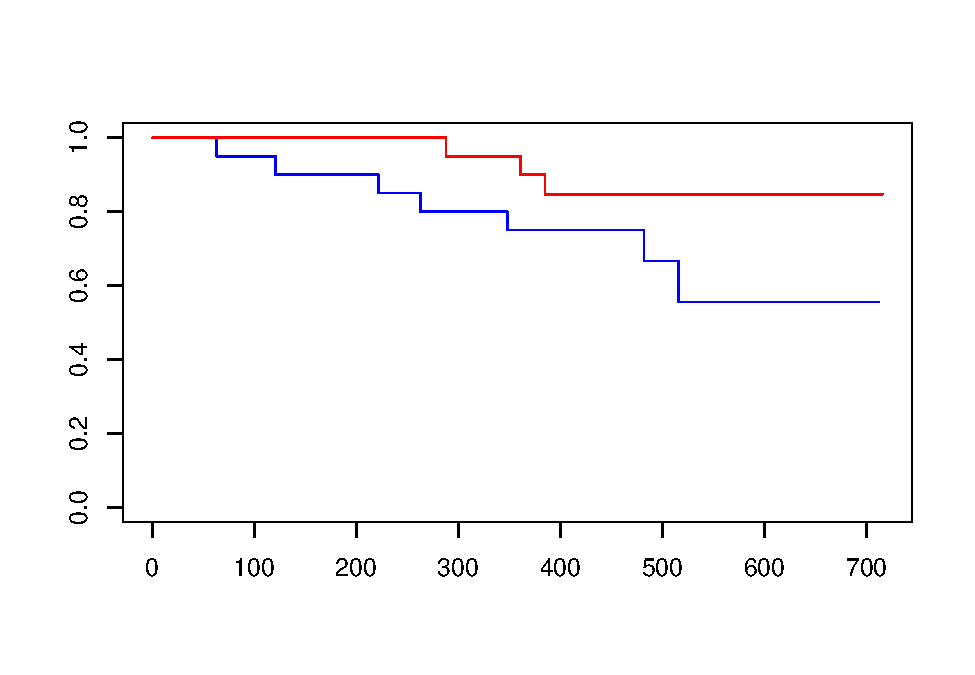
\includegraphics{09-answers_files/figure-latex/week7q-1.pdf}

Another way of doing this would be to estimate survival at say, 6, 12 and 18 months in each hospital. The command would be:

\begin{Shaded}
\begin{Highlighting}[]
\KeywordTok{summary}\NormalTok{(}\KeywordTok{survfit}\NormalTok{(}\KeywordTok{Surv}\NormalTok{(lesson7b}\OperatorTok{$}\NormalTok{time, lesson7b}\OperatorTok{$}\NormalTok{recurrence) }\OperatorTok{~}\StringTok{ }\NormalTok{lesson7b}\OperatorTok{$}\NormalTok{hivolume),}
        \DataTypeTok{times =} \KeywordTok{c}\NormalTok{(}\DecValTok{183}\NormalTok{, }\DecValTok{365}\NormalTok{, }\DecValTok{548}\NormalTok{))}
\end{Highlighting}
\end{Shaded}

\begin{verbatim}
## Call: survfit(formula = Surv(lesson7b$time, lesson7b$recurrence) ~ 
##     lesson7b$hivolume)
## 
##                 lesson7b$hivolume=0 
##  time n.risk n.event survival std.err lower 95% CI upper 95% CI
##   183     18       2    0.900  0.0671        0.778        1.000
##   365     15       3    0.750  0.0968        0.582        0.966
##   548      5       2    0.556  0.1404        0.339        0.912
## 
##                 lesson7b$hivolume=1 
##  time n.risk n.event survival std.err lower 95% CI upper 95% CI
##   183     20       0    1.000  0.0000        1.000            1
##   365     18       2    0.900  0.0671        0.778            1
##   548     10       1    0.847  0.0814        0.702            1
\end{verbatim}

You could report survival of 100\%, 90\%, and 85\% in the high volume hospital compared to 90\%, 75\% and 56\% in the low volume hospital.

\hypertarget{lesson7c.rds}{%
\subsection{lesson7c.rds}\label{lesson7c.rds}}

\textbf{These are data from a randomized trial comparing no treatment, 5FU (a chemotherapy agent) and 5FU plus levamisole in the adjuvant treatment of colon cancer. Describe the data set. What conclusions would you draw about the effectiveness of the different treatments?}

Let's jump straight to the model answer.

The study consisted of 929 patients, of whom 452 died during the study. Median duration of follow-up for survivors was 6.4 years. Median survival in the control and 5FU groups was 5.7 and 5.9, respectively; median survival for the combination group has not been reached (see figure). The overall log-rank test was significant (p=0.003), suggesting that the survival is different between groups. In a multivariable Cox regression with group coded as two dummy variables (5FU and Levamisole), 5FU was found to have little effect on survival (HR 0.97 (95\% CI 0.78, 1.21; p=0.8)). Levamisole, however, led to significantly increased survival (hazard ratio 0.69 (95\% CI 0.55, 0.87; p=0.002)).

\textbf{Figure}

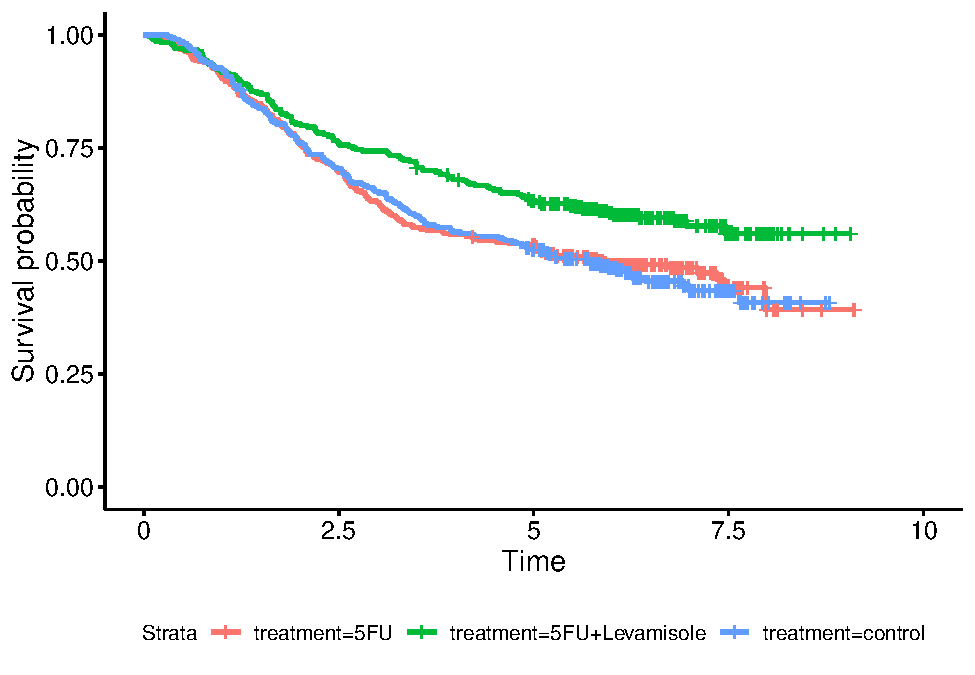
\includegraphics{09-answers_files/figure-latex/week7t-1.pdf}

In case you are wondering how I did all this, one key is to see that in the dataset ``group'' and ``treatment'' are equivalent:

\begin{Shaded}
\begin{Highlighting}[]
\KeywordTok{tbl_summary}\NormalTok{(}
\NormalTok{  lesson7c }\OperatorTok\StringTok{ }\KeywordTok{select}\NormalTok{(group, treatment),}
  \DataTypeTok{by =} \StringTok{"treatment"}
\NormalTok{)}
\end{Highlighting}
\end{Shaded}

\captionsetup[table]{labelformat=empty,skip=1pt}
\begin{longtable}{lccc}
\toprule
\textbf{Characteristic}\textsuperscript{1} & \textbf{5FU}, N = 310 & \textbf{5FU+Levamisole}, N = 304 & \textbf{control}, N = 315 \\ 
\midrule
group &  &  &  \\ 
1 & 0 (0\%) & 0 (0\%) & 315 (100\%) \\ 
2 & 310 (100\%) & 0 (0\%) & 0 (0\%) \\ 
3 & 0 (0\%) & 304 (100\%) & 0 (0\%) \\ 
\bottomrule
\end{longtable}
\vspace{-5mm}
\begin{minipage}{\linewidth}
\textsuperscript{1}Statistics presented: n (\%) \\ 
\end{minipage}

When I did the graph, I used the variable ``treatment'' to get the names of the treatments (rather than the group number). I also used a function called \texttt{ggsurvplot} (from the \texttt{survminer} package) rather than the standard \texttt{plot} option, because \texttt{ggsurvplot} allows more customization to the graph.

\begin{Shaded}
\begin{Highlighting}[]
\KeywordTok{ggsurvplot}\NormalTok{(}\KeywordTok{survfit}\NormalTok{(}\KeywordTok{Surv}\NormalTok{(survival_time}\OperatorTok{/}\FloatTok{365.25}\NormalTok{, died) }\OperatorTok{~}\StringTok{ }\NormalTok{treatment, }\DataTypeTok{data =}\NormalTok{ lesson7c),}
           \DataTypeTok{legend =} \StringTok{"bottom"}\NormalTok{)}
\end{Highlighting}
\end{Shaded}

When I did the Cox regression, I created dummy variables by typing:

\begin{Shaded}
\begin{Highlighting}[]
\NormalTok{lesson7c <-}
\StringTok{  }\NormalTok{lesson7c }\OperatorTok
\StringTok{  }\KeywordTok{mutate}\NormalTok{(}
    \DataTypeTok{fu =} \KeywordTok{if_else}\NormalTok{(group }\OperatorTok{==}\StringTok{ }\DecValTok{2}\NormalTok{, }\DecValTok{1}\NormalTok{, }\DecValTok{0}\NormalTok{),}
    \DataTypeTok{lev =} \KeywordTok{if_else}\NormalTok{(group }\OperatorTok{==}\StringTok{ }\DecValTok{3}\NormalTok{, }\DecValTok{1}\NormalTok{, }\DecValTok{0}\NormalTok{)}
\NormalTok{  )}
\end{Highlighting}
\end{Shaded}

Then it was straightforward to create the cox model and get the overall p-value from the \texttt{survdiff} function.

\begin{Shaded}
\begin{Highlighting}[]
\CommentTok{# Cox model}
\KeywordTok{coxph}\NormalTok{(}\KeywordTok{Surv}\NormalTok{(survival_time, died) }\OperatorTok{~}\StringTok{ }\NormalTok{fu }\OperatorTok{+}\StringTok{ }\NormalTok{lev, }\DataTypeTok{data =}\NormalTok{ lesson7c)}
\end{Highlighting}
\end{Shaded}

\begin{verbatim}
## Call:
## coxph(formula = Surv(survival_time, died) ~ fu + lev, data = lesson7c)
## 
##         coef exp(coef) se(coef)      z       p
## fu  -0.02664   0.97371  0.11030 -0.241 0.80917
## lev -0.37171   0.68955  0.11875 -3.130 0.00175
## 
## Likelihood ratio test=12.15  on 2 df, p=0.002302
## n= 929, number of events= 452
\end{verbatim}

\begin{Shaded}
\begin{Highlighting}[]
\CommentTok{# Overall p-value}
\KeywordTok{survdiff}\NormalTok{(}\KeywordTok{Surv}\NormalTok{(survival_time, died) }\OperatorTok{~}\StringTok{ }\NormalTok{group, }\DataTypeTok{data =}\NormalTok{ lesson7c)}
\end{Highlighting}
\end{Shaded}

\begin{verbatim}
## Call:
## survdiff(formula = Surv(survival_time, died) ~ group, data = lesson7c)
## 
##           N Observed Expected (O-E)^2/E (O-E)^2/V
## group=1 315      168      148      2.58      3.85
## group=2 310      161      146      1.52      2.25
## group=3 304      123      157      7.55     11.62
## 
##  Chisq= 11.7  on 2 degrees of freedom, p= 0.003
\end{verbatim}

Any oncologists notice a problem here? It is this: Levamisole doesn't work at all, but 5FU (obviously) does. It turns out that this whole data set (which I downloaded from the internet) was miscoded: it should have been: control, levamisole alone, levamisole + 5FU. Which goes to show the importance of checking your data.

\hypertarget{lesson7d.rds}{%
\subsection{lesson7d.rds}\label{lesson7d.rds}}

\textbf{More data on time to recurrence by hospital volume. Given this data set, determine whether patients treated at a ``high volume'' hospital have a longer time to recurrence.}

These data are comparable to lesson7b.rds, except with a longer length of follow-up. There are more recurrences (events) because more time has elapsed. So though the hazard ratio is very similar, and the number of patients identical, the confidence interval is much narrower and the results statistically significant. However, do be careful about drawing causal inferences: just because recurrence rates are lower at the high volume hospital, it doesn't mean that treatment at a high volume hospital reduces risk of recurrence. There may be other differences between hospitals (e.g.~case mix).

\hypertarget{exam}{%
\chapter{Exam}\label{exam}}

\hypertarget{question-1}{%
\section{Question 1}\label{question-1}}

I have provided a data set (``exam 01'') in two formats: R (.rds) and Excel. The excel file consists of two worksheets, one with the data, and another describing what the variables are. The data are from a study of advanced prostate cancer. The investigators are studying the ``bone scan index'', a new way of quantifying the extent of metastatic disease. They want to see whether the index predicts survival (I didn't include survival data in the data set because we aren't going to analyze that). What I'd like you to do is create a ``table 1'' to describe the study cohort. You can either do this by analyzing real data or by explaining what you'd do. As a hypothetical illustration, if I'd sent you data from a study on pain, you could either send me:

1:

\textbf{Table 1. Characteristics of sample. Data are mode (range) or percentage.}

\captionsetup[table]{labelformat=empty,skip=1pt}
\begin{longtable}{ll}
\toprule
Characteristic & Statistic \\ 
\midrule
Mean baseline pain & 4.5 (1.4 - 45) \\ 
Mean post-treatment pain & 4.5 (1.4 - 45) \\ 
Women & 52\% \\ 
\bottomrule
\end{longtable}

2:

\textbf{Table 1. Characteristics of sample. Data are mode (range) or percentage.}

\captionsetup[table]{labelformat=empty,skip=1pt}
\begin{longtable}{ll}
\toprule
Characteristic & Statistic \\ 
\midrule
Mean baseline pain & ?? (?? - ??) \\ 
Mean post-treatment pain & ?? (?? - ??) \\ 
Women & ??\% \\ 
\bottomrule
\end{longtable}

Note that both of these tables are rather silly, I am just doing this for illustration. Your table should be in a format suitable for publication in a journal.

\hypertarget{question-2}{%
\section{Question 2}\label{question-2}}

Some colleagues of yours are working on a project to predict preoperatively which patients will be found to have positive lymph nodes. They send you the following print-out describing a logistic regression and give you the following: ``nodes is coded 1 for positive, 0 for negative; yos is year of surgery; age is in years; CA125 is in units of 10 μg/mL; histol is coded as 0, 1 or 2 whether the tumor was well differentiated, moderately differentiated or poorly differentiated on biopsy''.

\captionsetup[table]{labelformat=empty,skip=1pt}
\begin{longtable}{llllll}
\toprule
Covariate & Odds Ratio & Std. Err. & z & P>z & 95\% Conf. Interval \\ 
\midrule
yos & 1.026621 & 0.0168909 & 1.60 & 0.110 & 0.9940435, 1.060266 \\ 
age & 1.039007 & 0.0054137 & 7.34 & 0.000 & 1.02845, 1.049672 \\ 
CA125 & 1.04026 & 0.0051741 & 7.94 & 0.000 & 1.030169, 1.050451 \\ 
histol & 0.4306271 & 0.0292454 & -12.41 & 0.000 & 0.3769584, 0.4919369 \\ 
\bottomrule
\end{longtable}

Put this information in a format suitable for reporting in a journal article. Briefly state (in no more than 2 -- 3 sentences) any criticisms, comments or questions you might you offer your colleagues on their analysis.

\hypertarget{question-3}{%
\section{Question 3}\label{question-3}}

You read the following in a journal article:

\begin{quote}
There was no difference in progression-free survival (p=0.1433) between the group given platinum only therapy compared to those on platinum plus immunotherapy. Immunotherapy therefore does not improve progression-free survival for patients receiving platinum therapy for advanced lung cancer. In the correlative analysis, the serum marker YLK44 (p=0.0132) but not ELCA (p=0.0622), EPLA (p=0.7764), LDH (p=0.6475) nor PPR-3 (p=0.2150) was associated with response, defined as a 50\% or greater reduction in tumor size. We conclude that there is a statistically significant association between YLK44 and response rates in second-line therapy. Patients who responded to platinum (mean age 69, 95\% C.I. 62 to 76) were on average no younger than non-responders (mean age 73, 95\% C.I. 70 to 76).
\end{quote}

What errors of statistical analysis or interpretation can you find in this paragraph? Write out your answers \emph{briefly}, in bullet point form.

\hypertarget{question-4}{%
\section{Question 4}\label{question-4}}

Look through the PDF of the study on childhood cancer survivors. {[}{[}TODO: ADD LINK{]}{]} You don't have to read the discussion, or the second half of the results if you don't want, because the questions focus on the earlier part of the paper.

\begin{enumerate}
\def\labelenumi{\alph{enumi})}
\item
  Ignoring the first section of the results on patient characteristics, and the associated table 1, what is the null hypothesis associated with the first statistical test reported in the paper? You don't have worry too much about working out exactly which null hypothesis is the first one, a null hypothesis somewhere near the beginning will do.
\item
  Look at table 2. Write two brief bullet points commenting on the statistical methods used in the table and / or the conclusions that the authors draw from the data presented in the table.
\end{enumerate}


\end{document}
